\documentclass[a4paper, 12pt,oneside]{article}
%fleqn

%On peut changer "oneside" en "twoside" si on sait que le résultat sera recto-verso.
%Cela influence les marges (pas ici car elles sont identiques à droite et à gauche)

% pour l'inclusion de figures en eps,pdf,jpg,....
\usepackage{graphicx}
 \usepackage{enumitem}
%Marges. Désactiver pour utiliser les valeurs LaTeX par défaut
%\usepackage[top=2.5cm, bottom=2cm, left=2cm, right=2cm, showframe]{geometry}
\usepackage[top=2.5cm, bottom=2.5cm, left=2cm, right=2cm]{geometry}


% quelques symboles mathematiques en plus
\usepackage{amsmath}


%\usepackage[squaren,Gray]{SIunits}
\usepackage{siunitx}
% le tout en langue francaise
\usepackage[anglais]{babel}

% on peut ecrire directement les charactères avec l'accent
\usepackage[T1]{fontenc}

\usepackage{array,multirow,makecell}
\usepackage{graphicx}
\usepackage[svgnames]{xcolor}
\usepackage{colortbl}

% a utiliser sur Linux/Windows
%\usepackage[latin1]{inputenc}

% a utiliser avec UTF8
\usepackage[utf8]{inputenc}
%Très utiles pour les groupes mixtes mac/PC. Un fichier texte enregistré sous codage UTF-8 est lisible dans les deux environnement.
%Plus de problème de caractères accentués et spéciaux qui ne s'affichent pas

% a utiliser sur le Mac
%\usepackage[applemac]{inputenc}

% pour l'inclusion de liens dans le document (pdflatex)
\usepackage[colorlinks,bookmarks=false,linkcolor=black,urlcolor=blue, citecolor=black]{hyperref}
%\usepackage{table}
%Pour l'utilisation plus simple des unités et fractions
\usepackage{units}
\usepackage{setspace}
\usepackage{float}
\usepackage{caption}
%Pour utiliser du time new roman... Comenter pour utiliser du ComputerModern
%\usepackage{mathptmx}
%\usepackage{blindtext}
\usepackage[document]{ragged2e}
%Pour du code non interprété
\usepackage{verbatim}
\usepackage{verbdef}% http://ctan.org/pkg/verbdef
\bibliographystyle{unsrt}

%Pour changer la taille des titres de section et subsection. Ajoutez manuellement les autres styles si besoin.
\makeatletter
\renewcommand{\section}{\@startsection {section}{1}{\z@}%
             {-3.5ex \@plus -1ex \@minus -.2ex}%
             {2.3ex \@plus.2ex}%
             {\normalfont\normalsize\bfseries}}
\makeatother

\makeatletter
\renewcommand{\subsection}{\@startsection {subsection}{1}{\z@}%
             {-3.5ex \@plus -1ex \@minus -.2ex}%
             {2.3ex \@plus.2ex}%
             {\normalfont\normalsize\bfseries}}
\makeatother

\makeatletter
\newcommand{\scalefig}[3]{
  \begin{figure}[ht!]
    \centering
    \includegraphics[width=#2\columnwidth]{#1}
    %%% I think \captionwidth (see above) can go away as long as
    %%% \centering is above
    %\captionwidth{#2\columnwidth}%
    \caption{#3}
    \label{#1}
  \end{figure}}
\makeatother

%Début du document

\begin{document}


%Crée la page de titre
%\maketitle

%Ajoute la table des matières
%\tableofcontents
%Début du rapport à la page suivante
%\newpage

%De manière à ce que template latex ressemble au mieux au template word, on empêche latex de créer la page de titre et la créons à la main
%En taille de police 12, la commande \large donne une taille de police 14
%On utilise la commande \sffamily pour créer des caractères sans-serif
\begin{titlepage}

\newcommand{\HRule}{\rule{\linewidth}{0.5mm}} % Defines a new command for the horizontal lines, change thickness here

\begin{center} % Center everything on the page
 
%----------------------------------------------------------------------------------------
%	HEADING SECTIONS
%----------------------------------------------------------------------------------------



\includegraphics[scale=.1]{Images/logo-epfl.png}\\[0.5cm] % Include a department/university logo - this will require the graphicx package
\textsc{\Large Transportation Economics}\\[1.0cm] % 

%----------------------------------------------------------------------------------------
%	TITLE SECTION
%----------------------------------------------------------------------------------------

\HRule \\[0.4cm]
{ \huge  \textbf{Laboratory}}
\\
\bigbreak
{\huge Dynamic Traffic Modelling using METROPOLIS}\\[0.15cm] % Title of your document
\HRule \\[1.5cm]
\end{center}
%----------------------------------------------------------------------------------------
%	AUTHOR SECTION
%----------------------------------------------------------------------------------------
\noindent
\begin{minipage}[t]{1\textwidth}
\large

\emph{Author:}\\
François \textsc{BRUN}, SCIPER 297049 \\ Loris \textsc{DUCRY}, SCIPER 295906 \\
Grégoire \textsc{ECUYER}, SCIPER 263517 \\
Yifeng \textsc{CHEN}, SCIPER 336230 \\
% Your name
\end{minipage}

%-----
%	ABSTRACT SECTION
%----------------------------------------------------------------------------------------

\begin{center}
\hrule\vspace{0.5cm}
{
\center{\textbf{Synthesis}} \\
\justify


}\vspace{0.5cm}
\hrule
\vspace{1.cm}
%----------------------------------------------------------------------------------------
%	DATE SECTION
%----------------------------------------------------------------------------------------

{\large \today}\\[2cm] % Date, change the \today to a set date if you want to be precise

\vfill % Fill the rest of the page with whitespace
\end{center}
\end{titlepage}

\newpage
\tableofcontents

\newpage
\justify

\section{Introduction}

In this work, we will study different road pricing policies through a dynamic traffic model "Metropolis" in order to reduce congestion in a given network. We will be interested in evaluating and interpreting the characteristics of such a model, the results it brings in terms of congestion reduction and the variation of the latter following the modification of the input parameters.



\section{Task 1: Model Features}

\subsection{Network structure}

In the Metropolis simulator, we have a circular network made up of 4 rings and 8 axes, starting from the edge of the network and joining the centre of it. At each intersection of one of these axes with a ring, there is an intersection (a node) consisting of 4 branches.

Different types of thematic maps can be displayed on the network depending on the areas and links.

For zones, we can select departures, arrivals or averages.

For links, we can take lanes, lengths, speeds, capacities and types.

\begin{itemize}
    \item \underline{Departures}
\end{itemize}

Firstly, we can describe the structure of the network's departure areas.
The city centre is not really concerned because there is not really any housing there. This is the work area where people go in the morning.
We have the first ring of the network which is strongly affected by the departure areas. These are probably people living in the city, close to the city centre.
In the second ring, few people start their trips because it is an area between the city and the periphery where there is no (or little) housing.
In the third ring, we see the peri-urban residential areas.
Finally, in the fourth ring, there is again not much housing and therefore not much departure.

\begin{figure}[H]
    \centering
    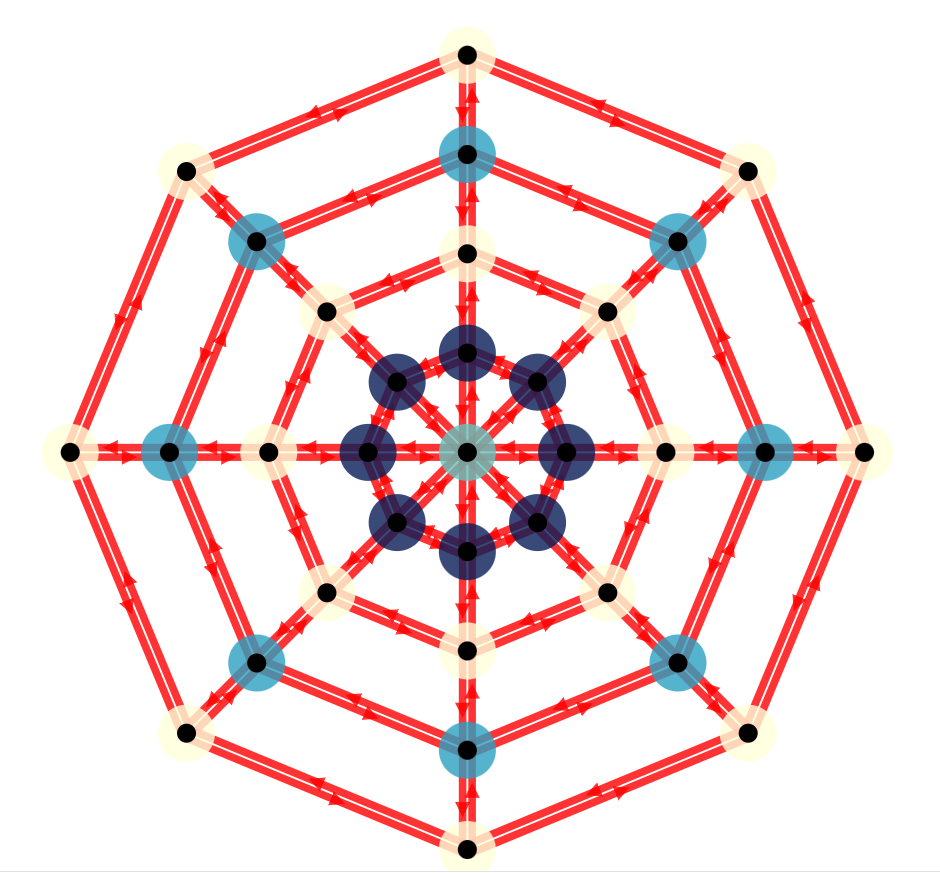
\includegraphics[width=0.5\textwidth]{Images/capture departure link.png}
    \caption{Network with starting areas and link structure}
\end{figure}

\begin{itemize}
    \item \underline{Arrivals}
\end{itemize}

Secondly, we can describe the structure of the incoming areas of the network.
We see a progressive effect of the network (with the maximum density in the city centre and very low (or no) density at the ends of the network).
This is simply due to the fact that in the morning rush hour, all inhabitants go to the city centre to work. As more and more jobs are located closer to the city centre, it is logical to observe an increasing density of passenger destinations.

\begin{figure}[H]
    \centering
    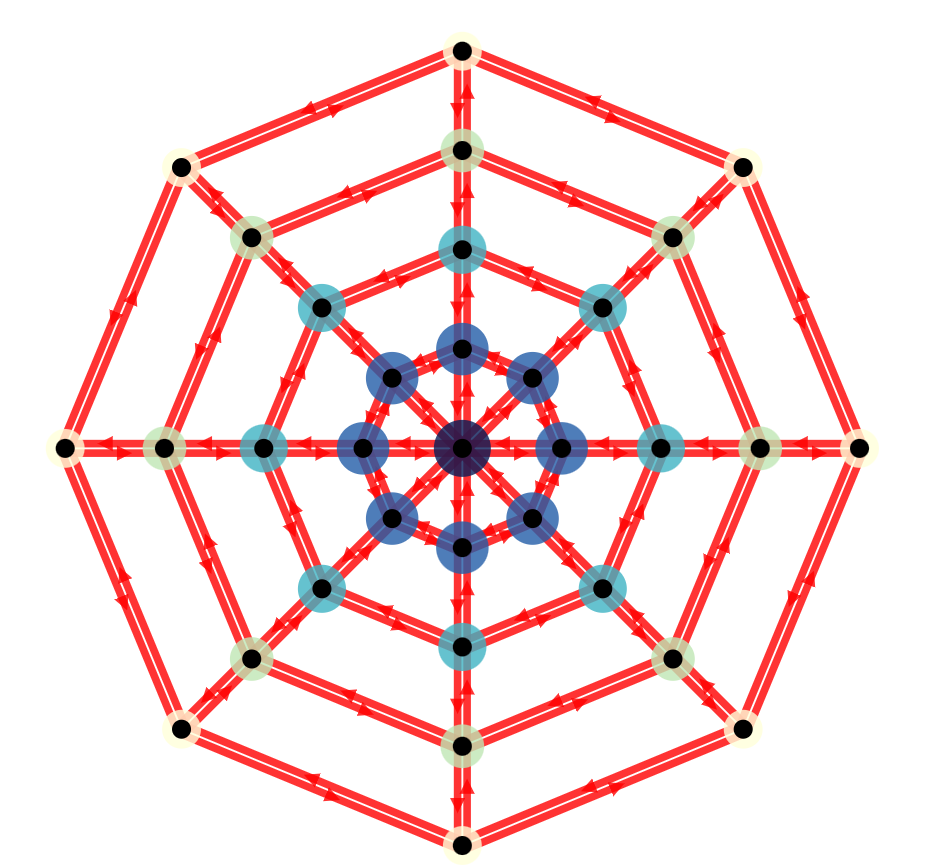
\includegraphics[width=0.5\textwidth]{Images/capture arrival link.png}
    \caption{Network with ending areas and link structure}
\end{figure}


%\begin{itemize}
%    \item \underline{Average}
%\end{itemize}



%\begin{figure}[H]
%    \centering
%    \includegraphics[width=0.5\textwidth]{Images/capture average link.png}
%    \caption{Network with average areas and link structure}
%\end{figure}

\begin{itemize}
    \item \underline{Lanes}
\end{itemize}

Third, we look at the structure of the network in terms of the number of traffic lanes per link. We find that there are two lanes per link on the radius roads (from the outside to the first ring road) and one lane per link on the ring roads and between the first ring road and the downtown area. This may be consistent with the fact that penetrating roads represent freeways while the others illustrate standard roads.
In the downtown area, there is only one lane per link since the highway ends before entering the downtown area.


\begin{figure}[H]
    \centering
    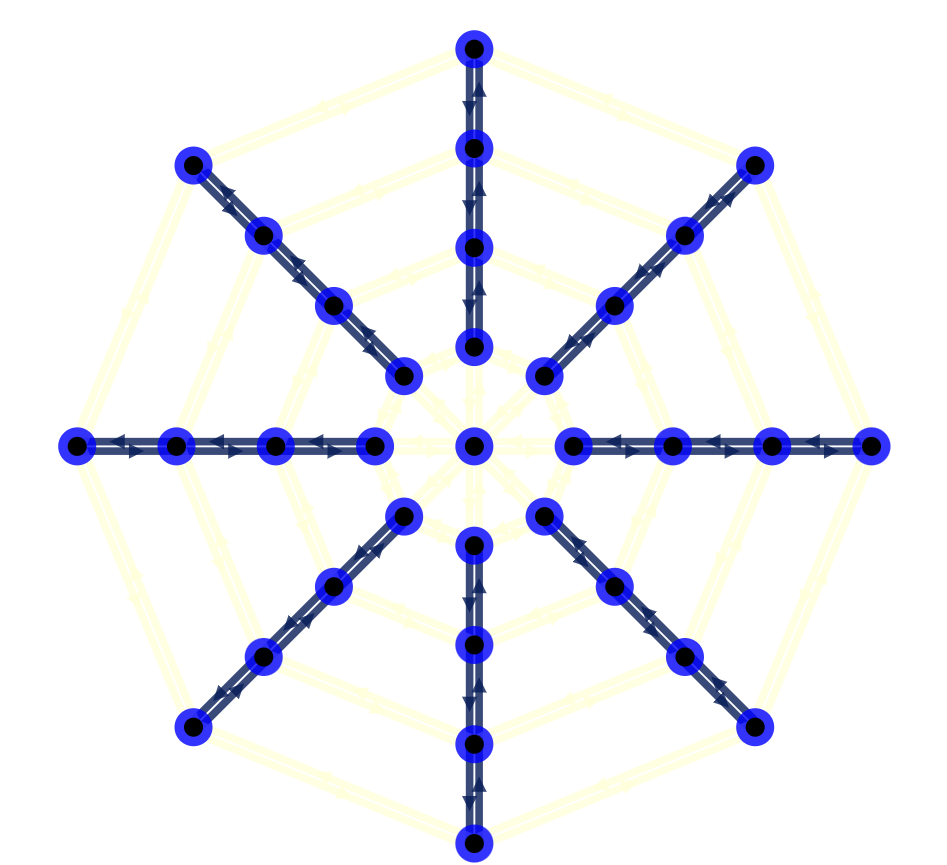
\includegraphics[width=0.5\textwidth]{Images/capture zone lane.png}
    \caption{Network with lanes and zones structure}
\end{figure}


\begin{itemize}
    \item \underline{Length}
\end{itemize}

Fourth, it is possible to look at the length of the roads. Clearly, the roads between the crowns have the same length and are therefore homogeneous.
Concerning the length of the links on the crowns, the further away from the centre, the greater the distance between the penetrating roads and the greater the length of the roads.

\begin{figure}[H]
    \centering
    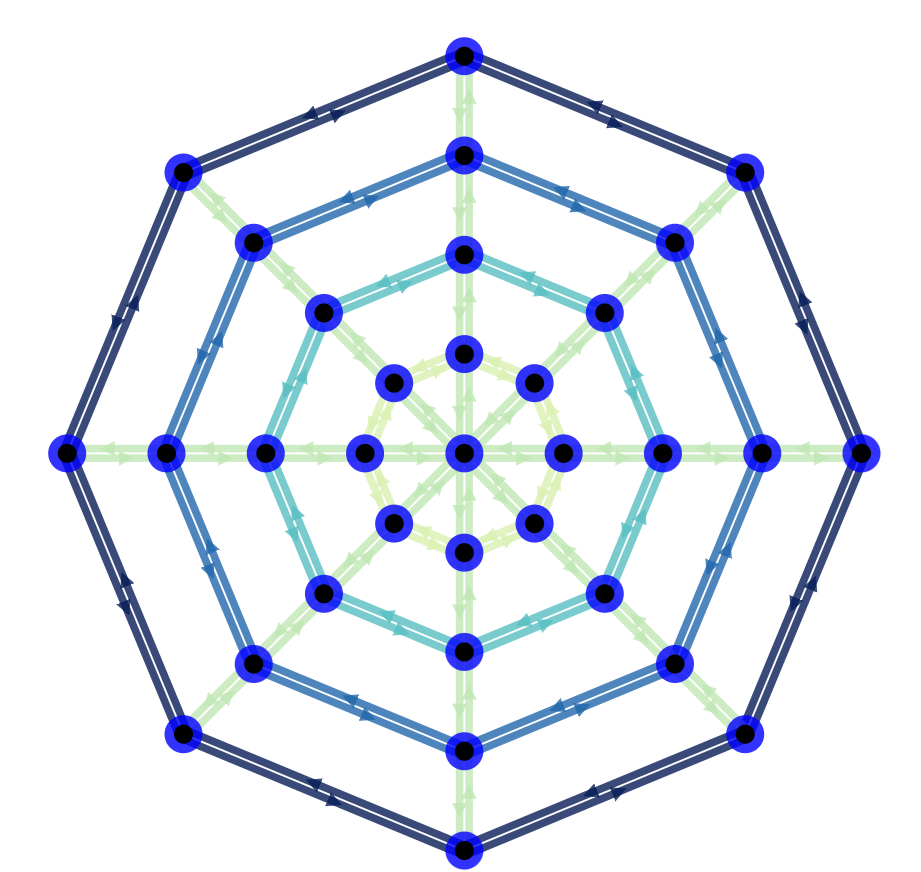
\includegraphics[width=0.5\textwidth]{Images/capture zone length.png}
    \caption{Network with length and zones structure}
\end{figure}

\begin{itemize}
    \item \underline{Speed}
\end{itemize}

In this part, we have the speed of each link illustrated.
For the roads that radially join the city centre, we have a speed of 70 [km/h], corresponding to high-speed roads. For the ring roads, we have a speed of 50 [km/h] which are secondary roads. In the downtown area, we have roads everywhere at 50 [km/h], corresponding to those observed in urban areas.

\begin{figure}[H]
    \centering
    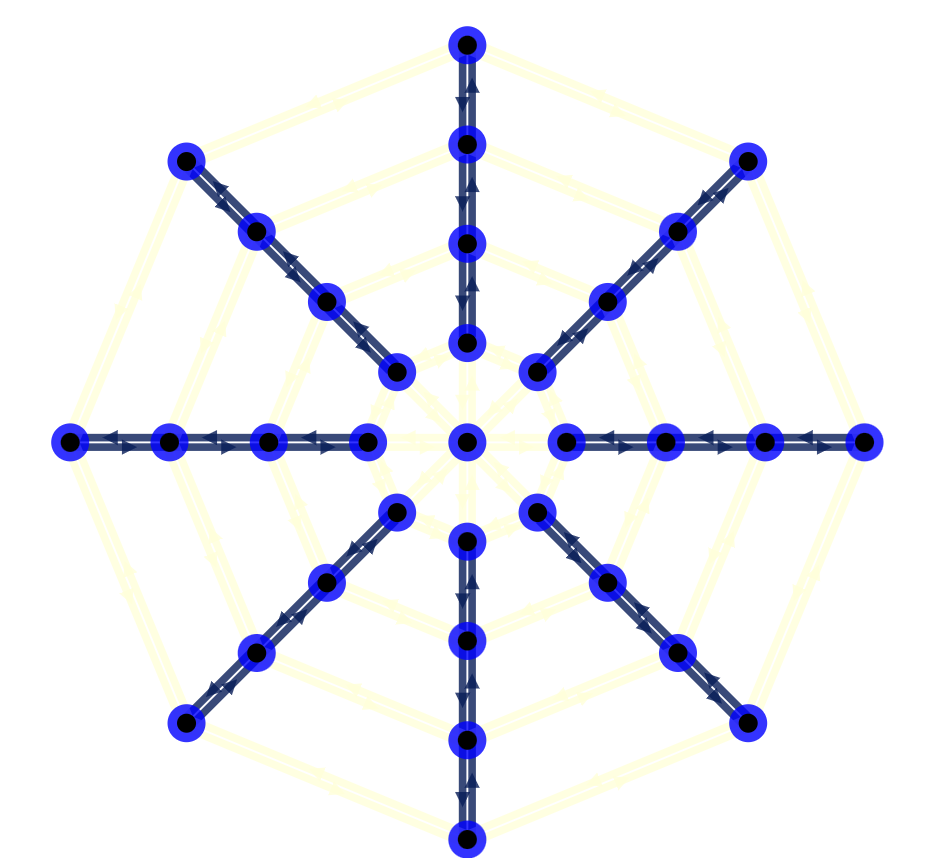
\includegraphics[width=0.5\textwidth]{Images/capture zone speed.png}
    \caption{Network with speeds and zones structure}
\end{figure}

\begin{itemize}
    \item \underline{Capacity}
\end{itemize}

This time we have the link capacity represented.
The capacity of the whole network is 2000 [veh/h/lane] except between the first ring and the city centre, where it is 3000 [veh/h/lane]. This seems logical since in this area there will be a significant amount of traffic to reach the city centre. Therefore, the capacity of the roads must be high enough to serve the users. This is also due to the fact that there were a lot of people living on the first ring road. As a result, outside of the inner ring, there will be less traffic and therefore less capacity.

\begin{figure}[H]
    \centering
    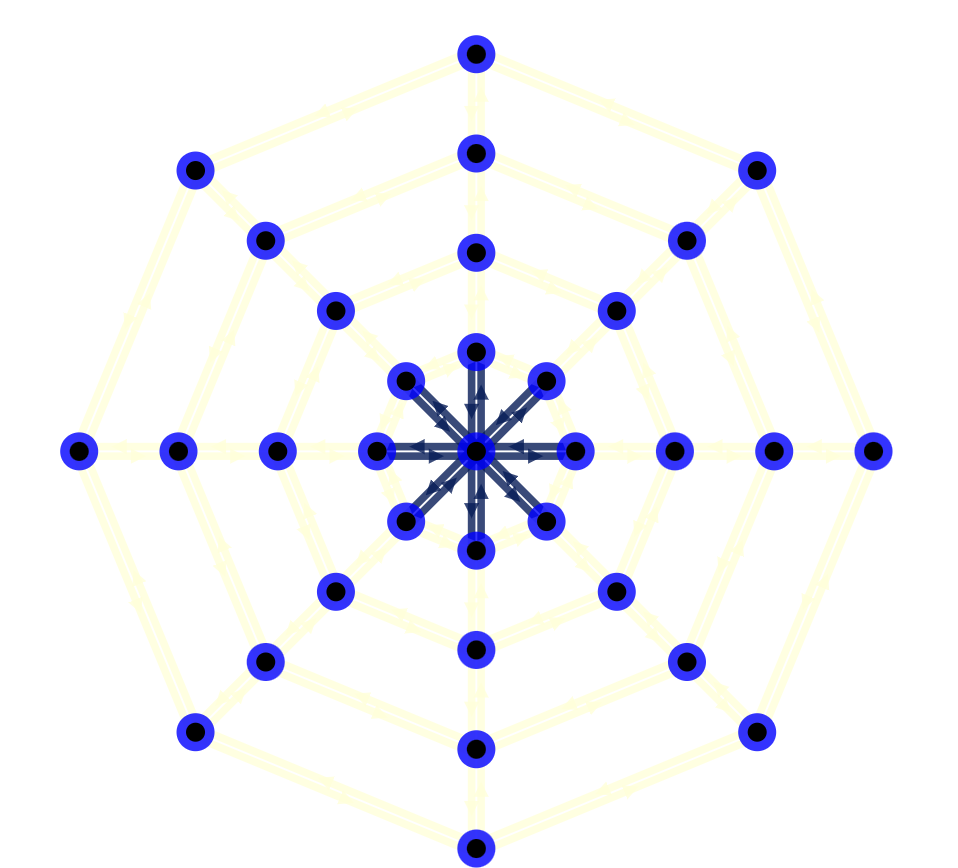
\includegraphics[width=0.5\textwidth]{Images/capture zone capacity.png}
    \caption{Network with capacities and zones structure}
\end{figure}

\begin{itemize}
    \item \underline{Type}
\end{itemize}

Finally, the last thing we can observe is the type of road we have.
In this case, we have only one type of link.

\begin{figure}[H]
    \centering
    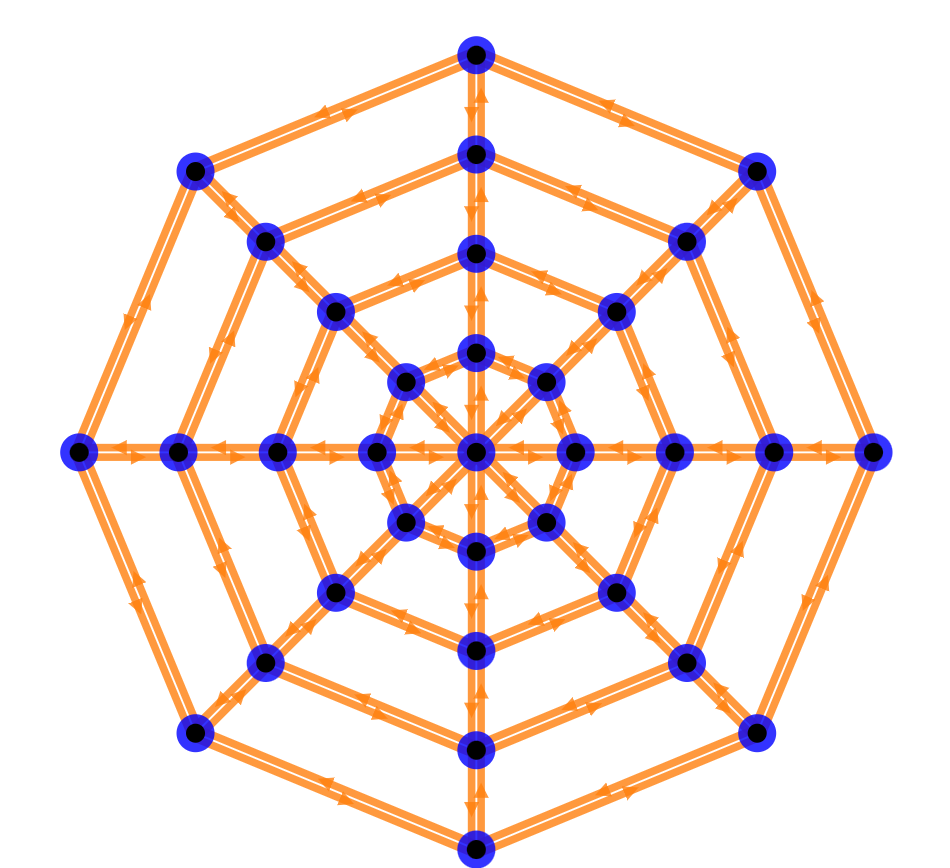
\includegraphics[width=0.5\textwidth]{Images/capture zone type.png}
    \caption{Network with types and zones structure}
\end{figure}




\subsection{Response to congestion}

\subsubsection{The description of congestion model}
The Metropolis congestion model is mesoscopic and combines aggregated congestion rules with individual vehicles to represent a macroscopic model of congestion. Each link is described by a congestion law, which is related to the link's current occupancy, incoming flow, and delay of travel time. This relationship, also known as the volume-delay function, is assessed by a vehicle joining or exiting a network link each time.

The travel time on a targeted link at time $t$ is given by

\begin{equation}
    tt(t)=f[dynVol(t), dynFlo(t); p_1, p_2, ...]
    \end{equation}
where:

\begin{itemize}
    \item $f$ is the function which explains the congestion law,
    \item $dynVol(t)$ represents the number of vehicles on the link at time $t$,
    \item $dynFlo(t)$ represents the incoming flow at the same moment,
    \item $p_1$, $p_2$, ... are the parameters defining the link (length, capacity, etc.).
\end{itemize}

\subsubsection{The implementation of congestion model}

In this part, the implementation of the congestion model is explained. Here 2 situations are considered: the bottleneck function and free flow function.

For the bottleneck function, the function is shown below:


\begin{equation}
    
tt=
\left\{
\begin{array}{cc}
   3600*(length/speed) & if \ dynVol<= lanes* capacity * length/speed  \\
   3600*(dynVol/capacity*lanes)) & else\\
\end{array}
\right.
\end{equation}
\\
where:
\begin{itemize}
    \item $tt$ is the total time of travel time,
    \item $length$ is the length of the link,
    \item $speed$ is the speed of the link,
    \item $capacity$ is the capacity of the link,
    \item $ lanes$ is the number of lanes of the link,
    \item $dynVol$ is the number of vehicles on the link
\end{itemize}
For the free flow situation, the function is shown below:
\begin{equation}
    tt=3600*(length/speed)
\end{equation}
where:
\begin{itemize}
    \item $tt$ is the total time of travel time,
    \item $length$ is the length of the link,
    \item $speed$ is the speed of the link,
    
\end{itemize}
\subsection{Traveler Features}
In this part, traveller features are introduced, they are:

\begin{itemize}
    \item modal choice (car or public transit),
    \item departure time choice (from the origin),
    \item route choice (before the departure and en-route choice),
    \item number of travellers.
\end{itemize}
\subsubsection{Modal choice}
For each O-D pair, Metropolis requires the travel duration by public transportation in order to calculate modal choice. Only certain demand segments are eligible for the modal option to be enabled. When enabled, a discrete choice model describes the modal option.

For a specific O-D pair, the generalized expense of public transportation is

\begin{equation}
    C_{PT}(O,D)=VOT_{PT}\cdot tt_{PT}(O,D)+P_{PT}
\end{equation}

where

\begin{itemize}
    \item $VOT_{PT}$ represents the value of time spent in public transportation (euros per hour),
    \item $tt_{PT}(O,D)$ represents the generalized travel time in public transportation from O to D (hour),
    \item $P_{PT}$ represents a fixed penalty associated with public transportation (euros).
\end{itemize}
The parameters $VOT_{PT}$ and $P_{PT}$ are specific to each traveller, while the travel time $tt_{PT}(O,D)$ is specified by the planner and is identical for every traveller.
\subsubsection{Departure choice}

Users must choose the time they want to leave home and start their trip.

Here are the parameters to consider when determining the departure time:

\begin{itemize}
    \item $tt(t)$ is the total travel time for a departure time t,
    \item $t^{*}$ is the desired arrival time at destination D,
    \item $\delta$ is the period during which users do not receive a penalty for their arrival time,
    \item $\alpha$ is the value of time in the car,
    \item $\beta$ is the penalty for arriving too early at the destination,
    \item $\gamma$ is the penalty for arriving too late at the destination
\end{itemize}

To model this, we use the following equation :

\begin{equation}
    C(t)= C_{1}(t) + C_{2}(t) + C_{3}(t)
    \end{equation}

where the first term is the travel time penalty :

\begin{equation}
    C_{1}(t)=\alpha\cdot tt(t)
    \end{equation}

the second term is the penalty for early arrival:

\begin{equation}
C_{2}(t)=
\left\{
\begin{array}{cc}
   \beta \cdot ((t^{*}-\delta/2)-(t+tt(t))) & if \ t + tt(t) < t^{*} - \delta/2  \\
   0 & if \ t + tt(t) \geq t^{*} - \delta/2
\end{array}
\right.
\end{equation}
\\

The third term is the late arrival penalty:

\begin{equation}
C_{3}(t)=
\left\{
\begin{array}{cc}
   \gamma \cdot ((t+tt(t))-(t^{*}+\delta/2)) & if \ t + tt(t) > t^{*} + \delta/2  \\
   0 &  if \  t + tt(t) \leq t^{*} + \delta/2
\end{array}
\right.
\end{equation}
\\

Since the model is stochastic (since the user will not necessarily choose the departure time generating the smallest cost), we will use the probability P(t), which follows a continuous logit model written as follows:

\begin{equation}
    P(t)dt=\frac{exp(-C(t)/\mu_{d})}{\int_{T_{0}}^{T_{1}}exp(-C(u)/\mu_{d})du}dt
    \end{equation}
where :
$\mu_{d}$ measures the heterogeneity of the departure time choice in the population

\subsubsection{Route Choice}

The route choice is based on a dynamic travel time model. The users have two types of information: historical travel time and instantaneous travel time. The historical one is the information that a user is collecting from one day to the next. He will change his behavior based on his learning process.

The user will make two types of choices:

\begin{itemize}
    \item pre-trip decisions: a decision on the departure time and one the route to make at the origin,
    \item en-route decisions: a decision on the direction for each intersection during the trip.
\end{itemize}

For the first term, it is only a matter of making a choice based on minimizing historical travel times.

For the second term, at each intersection, the user will see the travel time of each possible link of the intersection and will choose the one that allows him to minimize the time he has to do to reach his destination.

\begin{figure}[H]
    \centering
    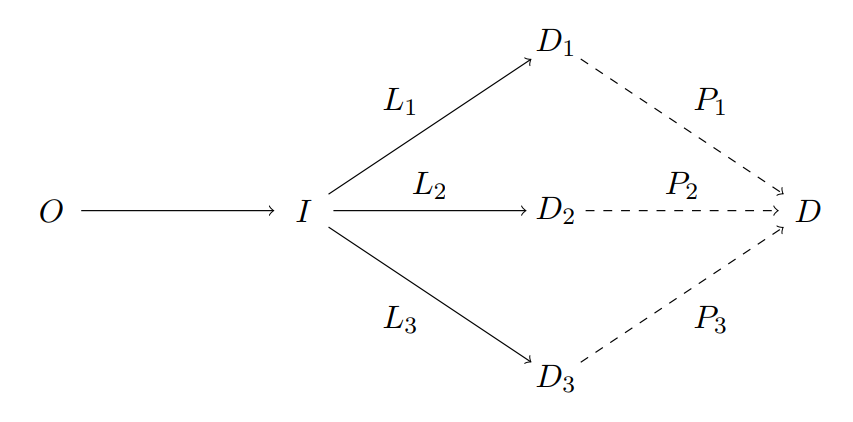
\includegraphics[width=0.5\textwidth]{Images/capture route choice.png}
    \caption{Illustration of route choice at intersection I with 3 links $L_{j}$}
\end{figure}

The remaining time is thus the sum of the time it will take to travel to the chosen link plus the historically experienced travel time between the end of this link and the destination (at the time of entry into the chosen link (t) plus the time to travel there):

\begin{equation}
    tt_{j}(t)=tt^{S}_{L_{j}}(t) + tt^{H}_{P_{j}}(t+tt^{S}_{L_{j}}(t))
    \end{equation}

As for the choice of departure time, we use a probability based on a logit model according to the following relationship:

\begin{equation}
    P(i)=\frac{exp(-tt_{i}(t)/\mu_{r})}{\sum_{j=1}^{J}exp(-tt_{j}(t)/\mu_{r})}
    \end{equation}
where:\\
$J$ is the number of downstream links
\subsubsection{Number of Travelers}
To begin with, there is only one type of user, namely the "Standard Traveler".  There are 264,014 of them in the network. For each of them, it is possible to access the O-D matrix, in order to identify the origin and destination of each traveller's trip.

\section{Task 2: Output Features}

After exploring the data and operation of the "Metropolis" simulator, we will run a simulation with the following input parameters:

\begin{itemize}
    \item Stopping criterion: 50 iterations,
    \item Learning process: Exponential,
    \item Recording period: 6 AM - 11 AM,
    \item Time interval: 5 minutes,
\end{itemize}

Thanks to the results of the simulations, we will be able to analyse the propagation of congestion according to the analysis period as well as the evolution of the users' behaviour according to the iterations.

\subsection{Evolution of congestion during the analysis period}


Our analysis covers the period between 6 am and 11 am. Therefore, it covers the morning peak period when users travel from home to work. In order to carry out the requested analyses, we will use images of the simulation at different times of interest highlighting the entrance flows. Indeed, this parameter allows us to understand the saturation state of the network according to the flows entering each link.\\

\subsubsection{Learning Model}
In this section, the exponential learning process is implemented 
for minimising the total cost of travelling the whole network. The formula is shown below
\begin{equation}
    X^{H}(\omega+1) = (1-\lambda)X^{H}(\omega)+\lambda X^{S}(\omega)
\end{equation}

where:
\begin{itemize}
    \item $\omega$ represents the date,
    \item $\lambda$ represents the learning rate parameter,
    \item $X^{H}(\omega)$ represents the historical state in day $\omega$,
    \item $X^{S}(\omega)$ represents the simulated state in day $\omega$.
\end{itemize}
\subsubsection{Theoretical concepts from the lecture}
According to the lecture (dynamic models), the travel cost function of the no-toll condition is shown below:
\begin{equation}
    C(t)=\alpha(travel\ time)+\beta(time \ early)+\gamma(time\ late)
\end{equation}

Require $\beta$<$\alpha$.

Here we decide to implement the cost function based on this formula, which is already explained in section 2.3.2.

The formula above illustrates the cost of an individual traveller, the total travel time cost is shown below:
\begin{equation}
    TTC=\frac{\delta \cdot N^{2}}{2\cdot s }
\end{equation}
The total schedule delay cost is:
\begin{equation}
    SDC = \frac{\delta \cdot N^{2}}{2\cdot s }
\end{equation}
where:
\begin{equation}
    \delta=\frac{\beta \cdot \gamma}{\beta+\gamma}
\end{equation}
Moreover, in order to simulate the behaviour of travellers each day, we decide to apply the logit model, which is shown in Formula 9. Therefore, a more diffused traveller behaviour could be obtained. 


\subsubsection{The simulation of congestion evolution}

In this task, the parameters of the model are shown below:

\begin{table}[]
    \centering
    \begin{tabular}{c|c}
        Name & Value \\
        \hline
        Number of traveller, $N$& 264014\\
        The value of the departure time $\mu$ & 2\\
        On-time window, $\delta$ & 10\\
        The value of time for public transportation & 15\\
        The value of time while driving, $\alpha$ & 10\\
        The early-arrival penalty, $\beta$ & 6\\
        The late-arrival penalty, $\gamma$ & 25\\
        Learning rate $\lambda$ & 0.1\\
        
    \end{tabular}
    \caption{The parameters table of task 2 simulation}
    \label{tab:The parameters table of task 2 simulation}
\end{table}
Then we get our simulation results.

First of all, we see that at the beginning of the simulation (at 6:00 am, \ref{fig:Entry flows in the network at 6:00 am}, there are very few flows (or even almost no traffic at all). We therefore start the day on a free network state.\\

\begin{figure}[H]
    \centring
    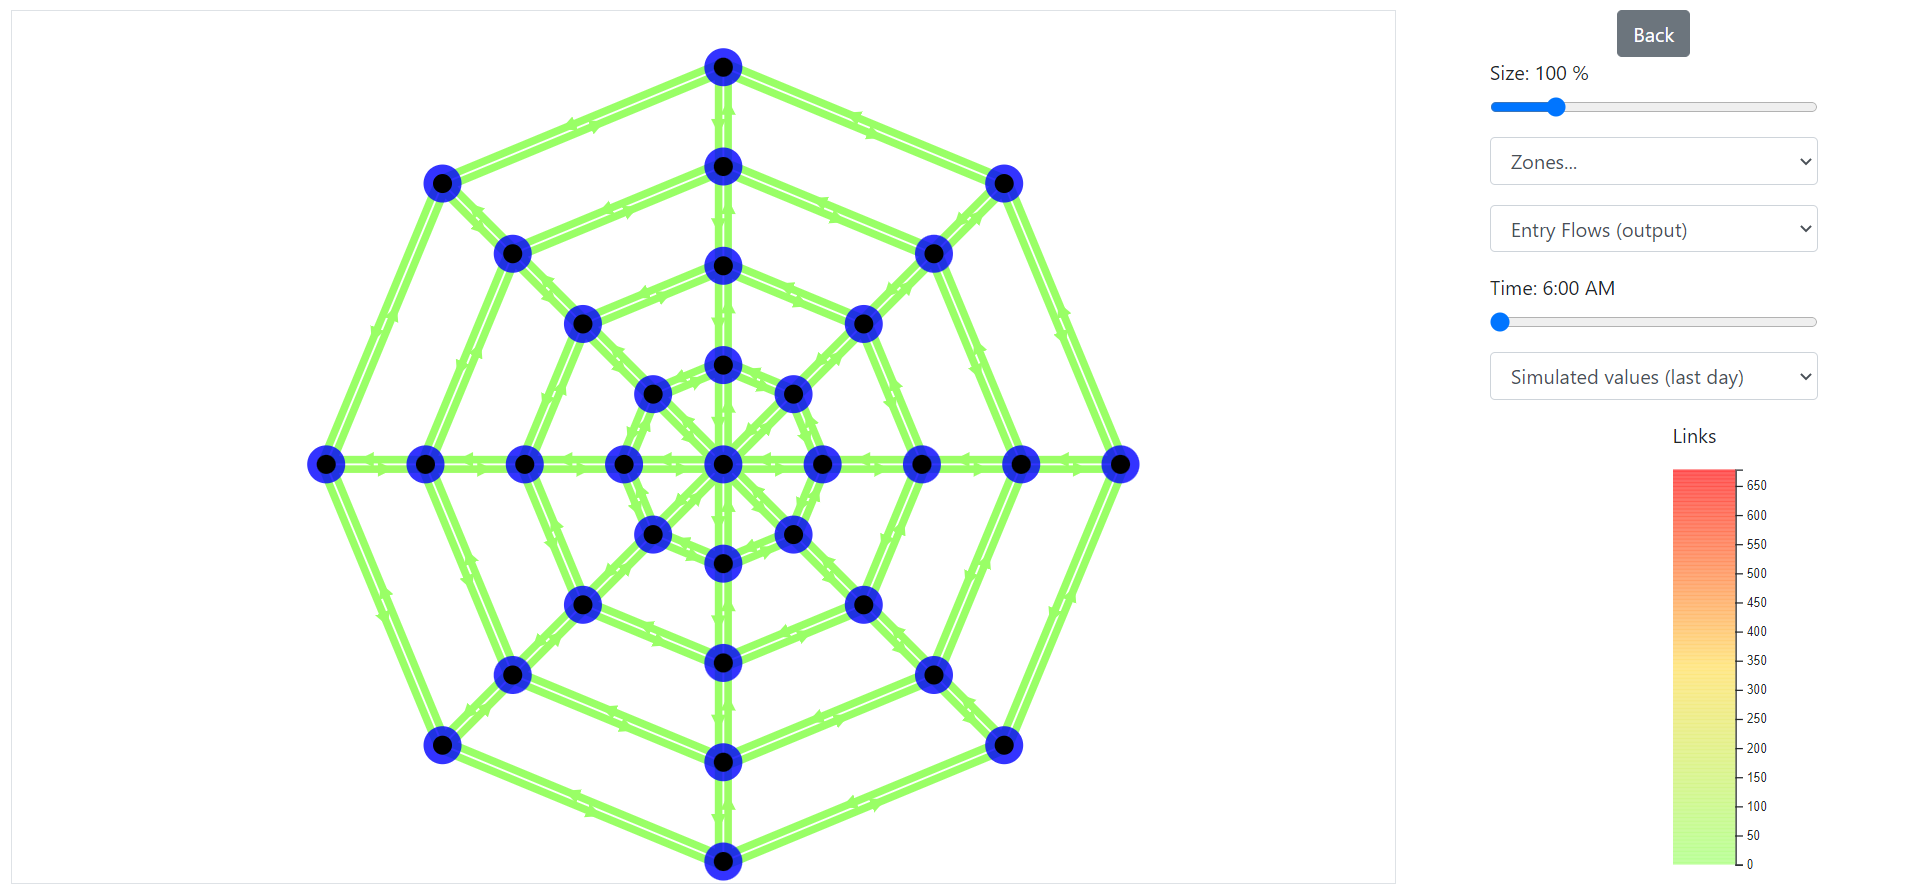
\includegraphics[width=1\textwidth]{Images/Step2/results_on_network_600am.png}
    \caption{Entry flows in the network at 6:00 am}
    \label{fig:Entry flows in the network at 6:00 am}
\end{figure}

Then, from 6:30 am, the roads leading to the centre of the network as well as the centre of the network itself start to record more important flows. The peak period starts at 6:45 am (\ref{fig:Entry flows in the network at 6:45 am}) and lasts until 7:10 am (\ref{fig:Entry flows in the network at 7:10 am}). During this period, we see strong flows from the edges of the network towards the centre of the network, which eventually fades away. It is therefore during this period that congestion is at its worst. This is consistent with the fact that it is during this period that the majority of users will be on the road to reach their work, most of them in the city centre. From 7:10 am until 8:15 am, the network remains fairly congested, due to the gradual disappearance of the congestion and the flows of workers who left later. Finally, after the period up to 8:30 am, during which there is still some flow, there is no more congestion at all until the end of the analyses (11:00 am).\\

\begin{minipage}[c]{0.5\textwidth}
\begin{figure}[H]
    \centering
    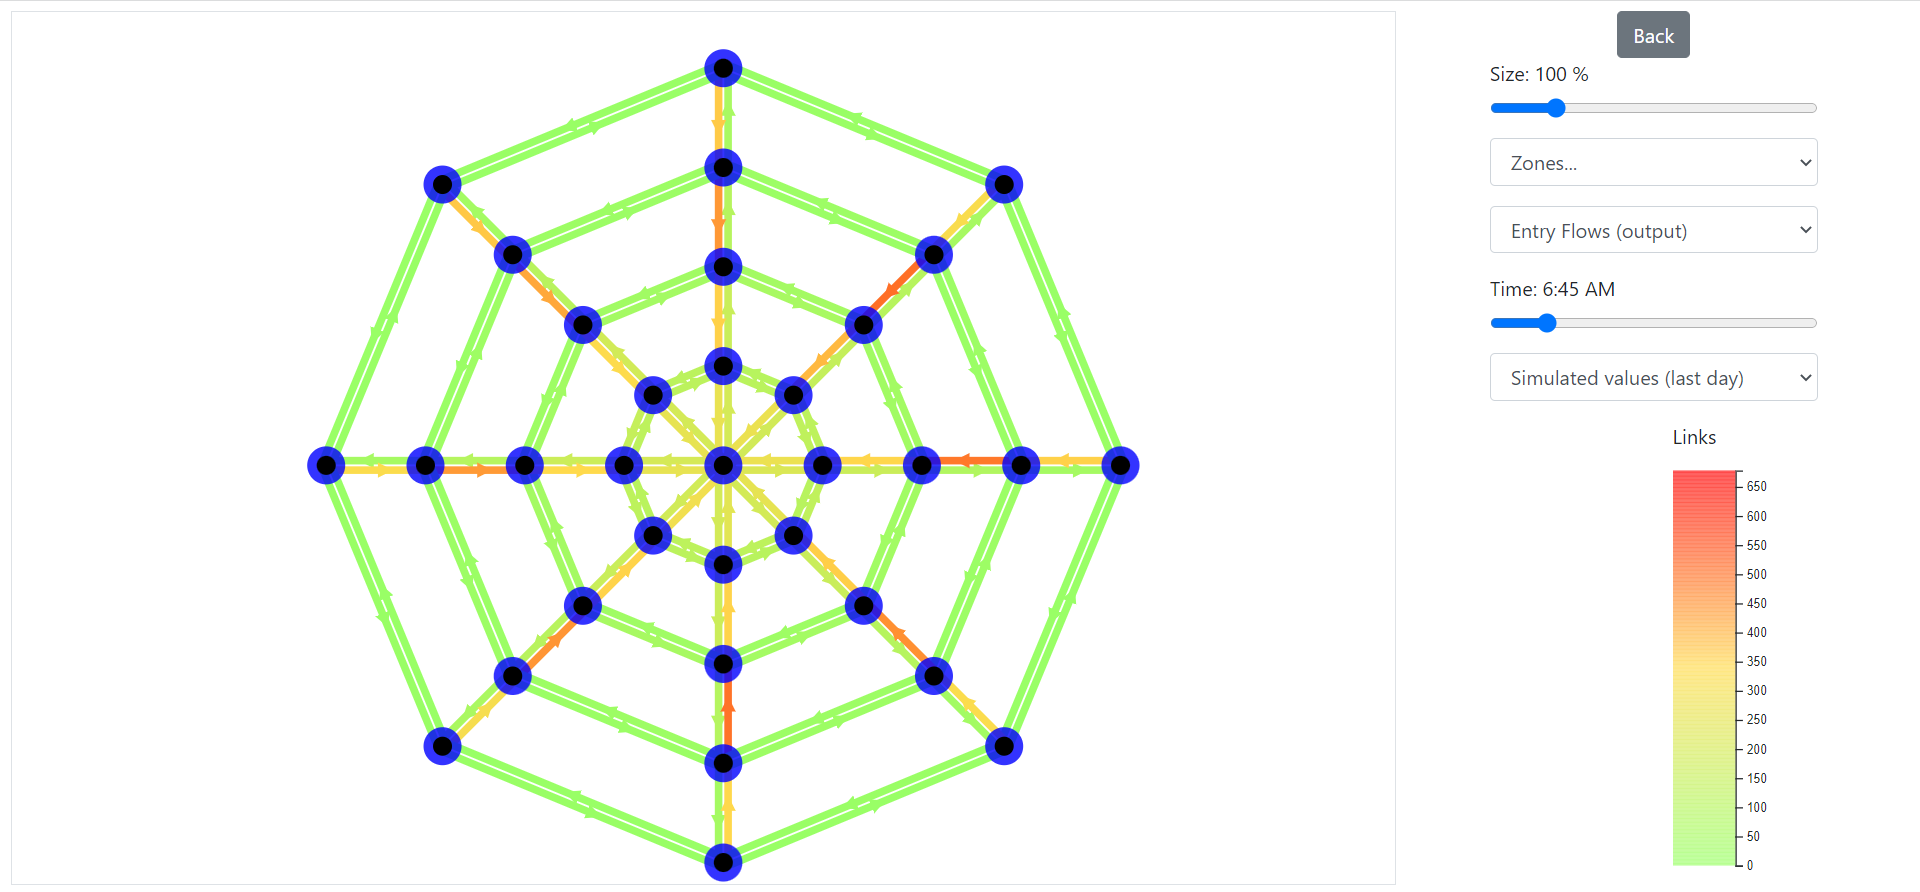
\includegraphics[width=1\textwidth]{Images/Step2/results_on_network_645am.png}
    \caption{Entry flows in the network at 6:45 am}
    \label{fig:Entry flows in the network at 6:45 am}
\end{figure}
\end{minipage}
\begin{minipage}[c]{0.5\textwidth}
\begin{figure}[H]
    \centering
    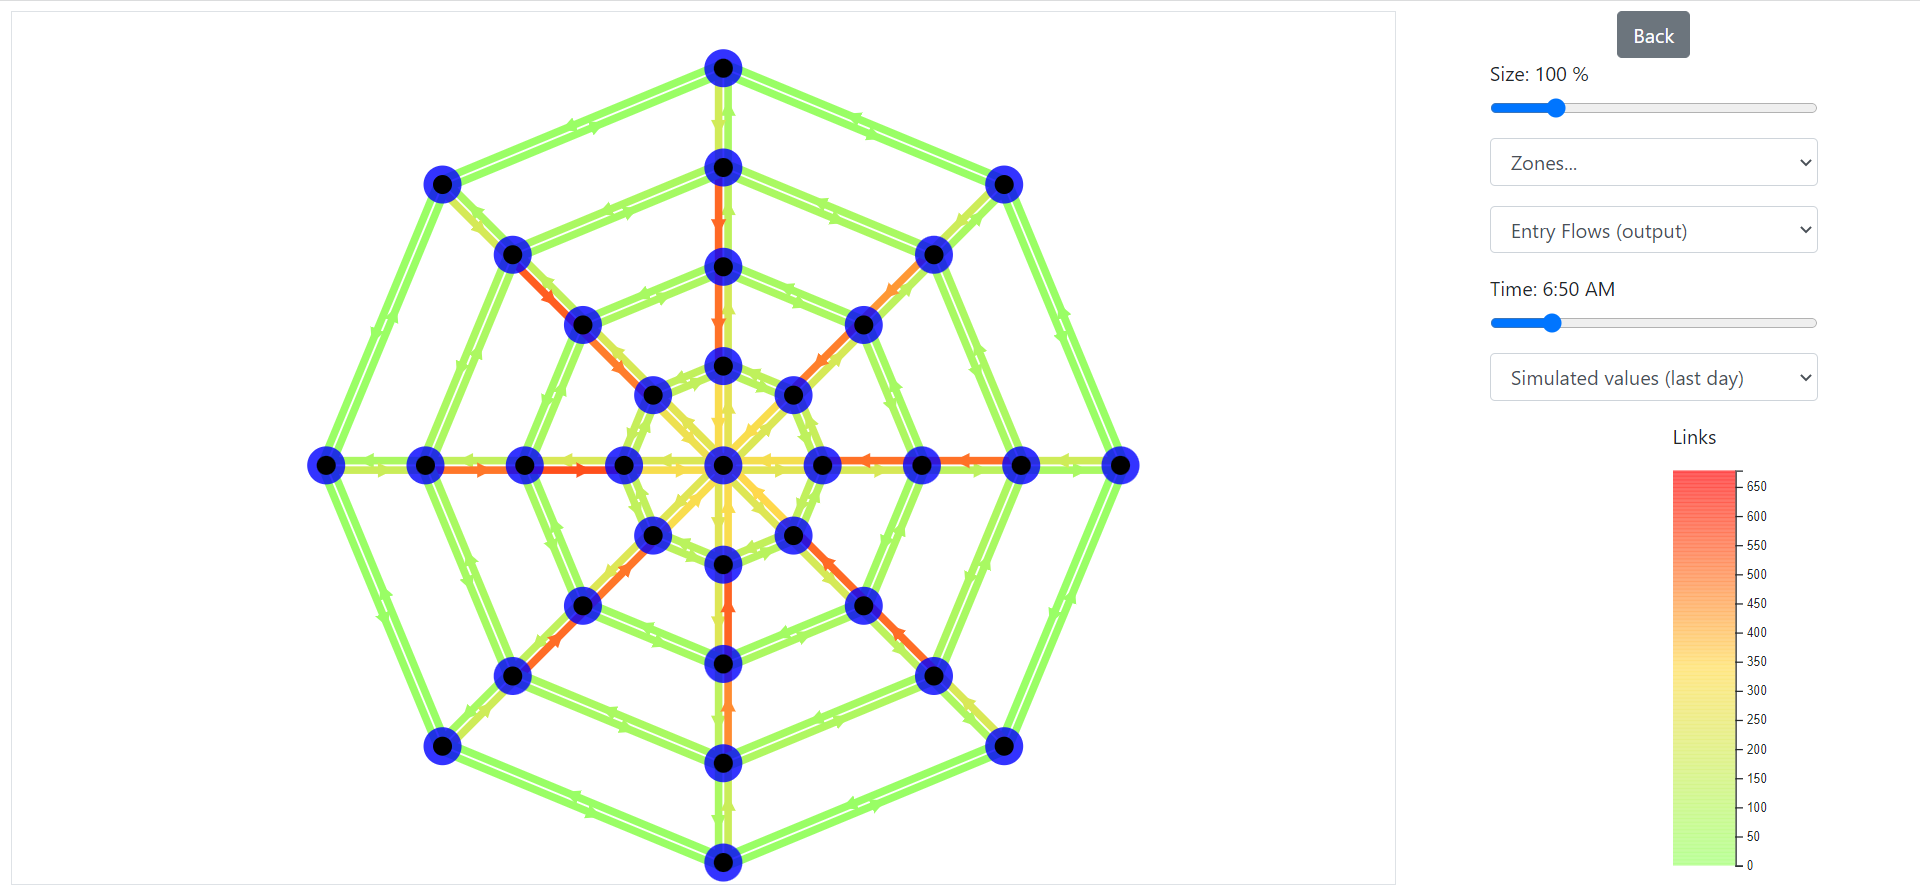
\includegraphics[width=1\textwidth]{Images/Step2/results_on_network_650am.png}
    \caption{Entry flows in the network at 6:50 am}
    \label{fig:Entry flows in the network at 6:50 am}
\end{figure}
\end{minipage}
\begin{minipage}[c]{0.5\textwidth}
\begin{figure}[H]
    \centering
    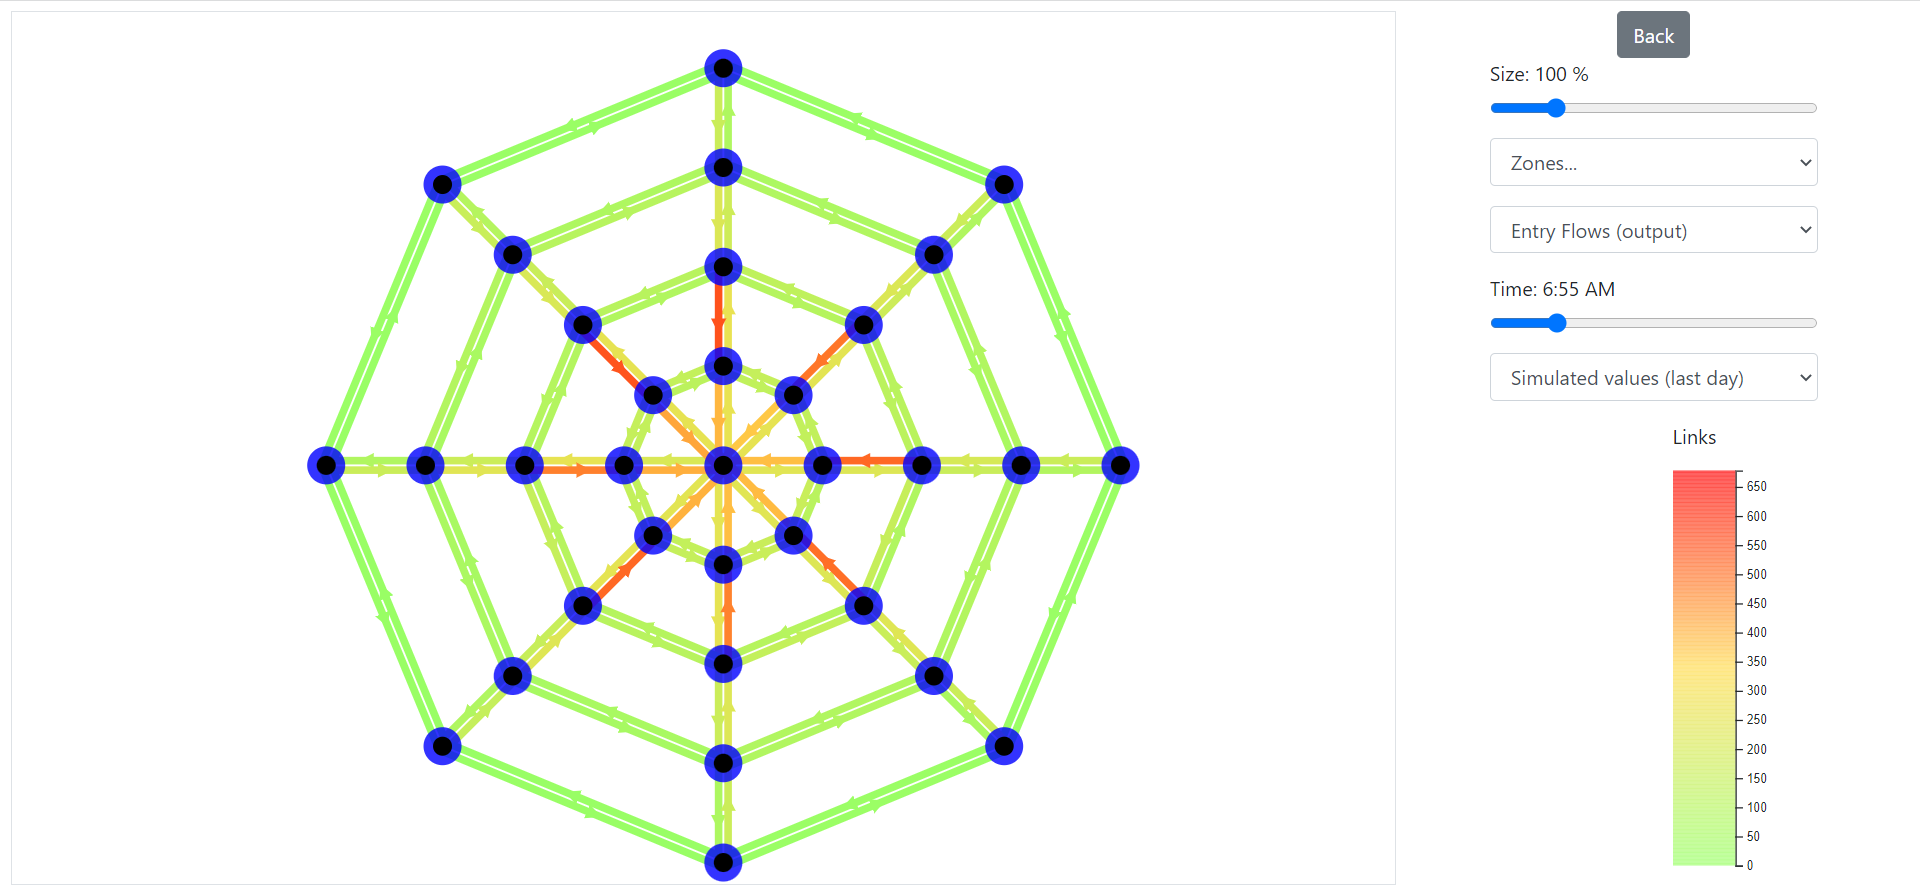
\includegraphics[width=1\textwidth]{Images/Step2/results_on_network_655am.png}
    \caption{Entry flows in the network at 6:55 am}
    \label{fig:Entry flows in the network at 6:55 am}
\end{figure}
\end{minipage}
\begin{minipage}[c]{0.5\textwidth}
\begin{figure}[H]
    \centering
    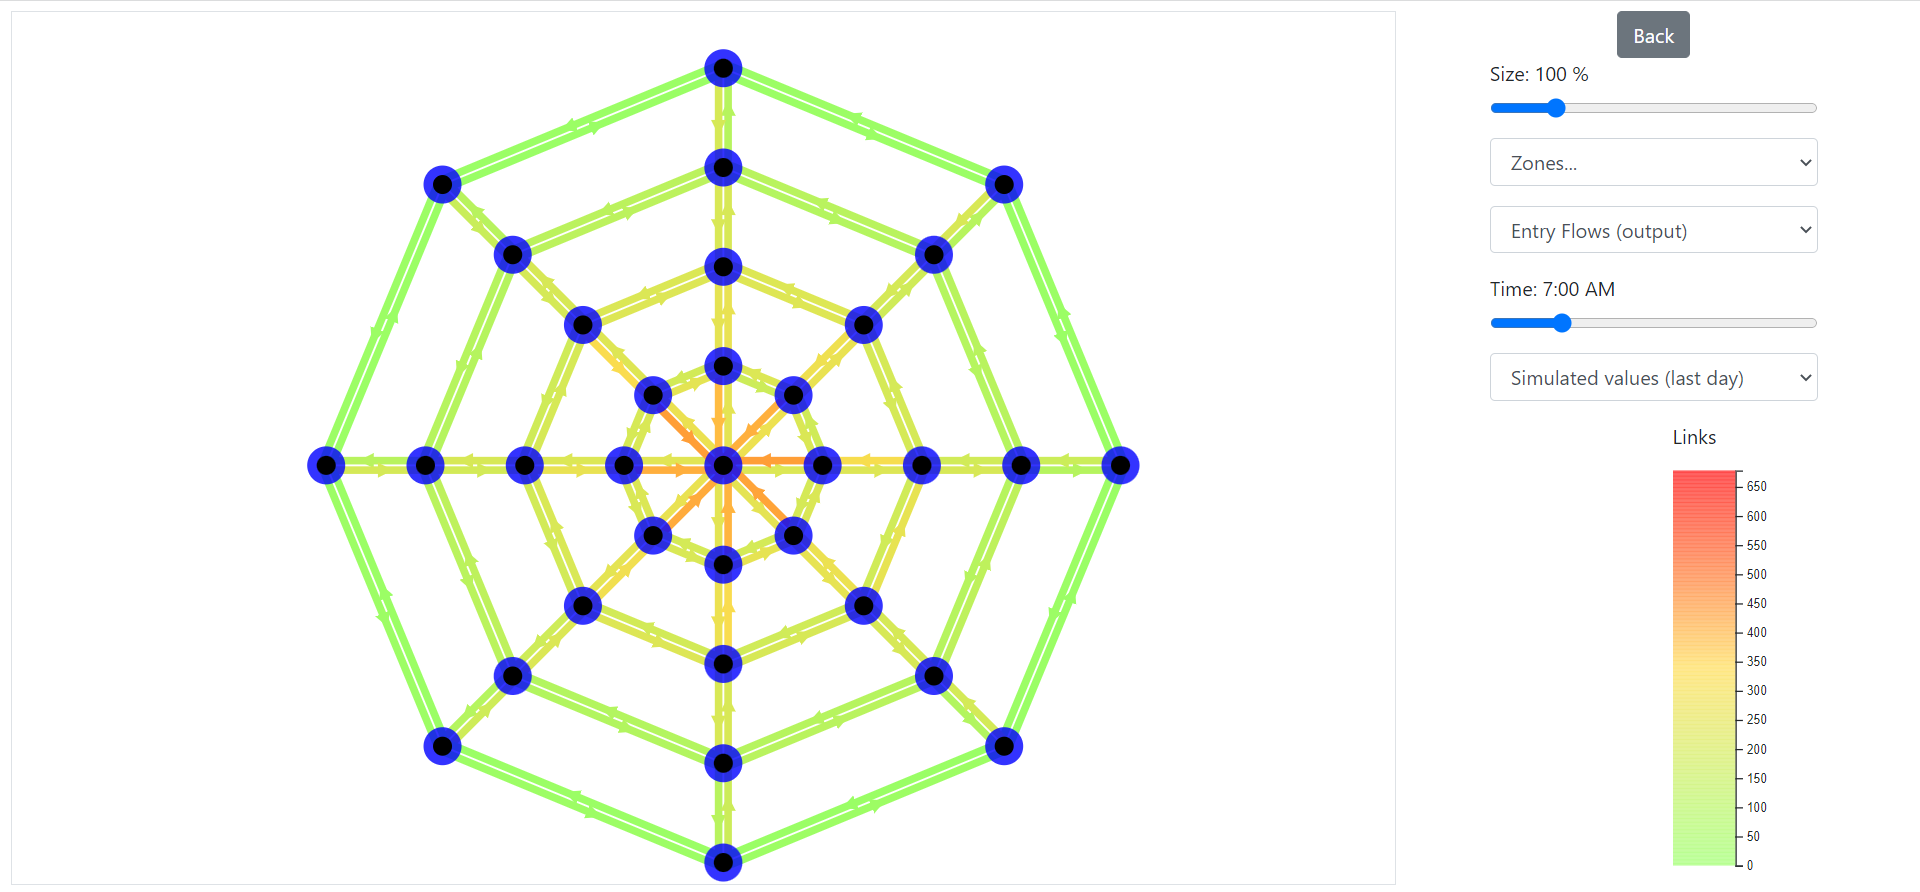
\includegraphics[width=1\textwidth]{Images/Step2/results_on_network_700am.png}
    \caption{Entry flows in the network at 7:00 am}
    \label{fig:Entry flows in the network at 7:00 am}
\end{figure}
\end{minipage}
\begin{minipage}[c]{0.5\textwidth}
\begin{figure}[H]
    \centering
    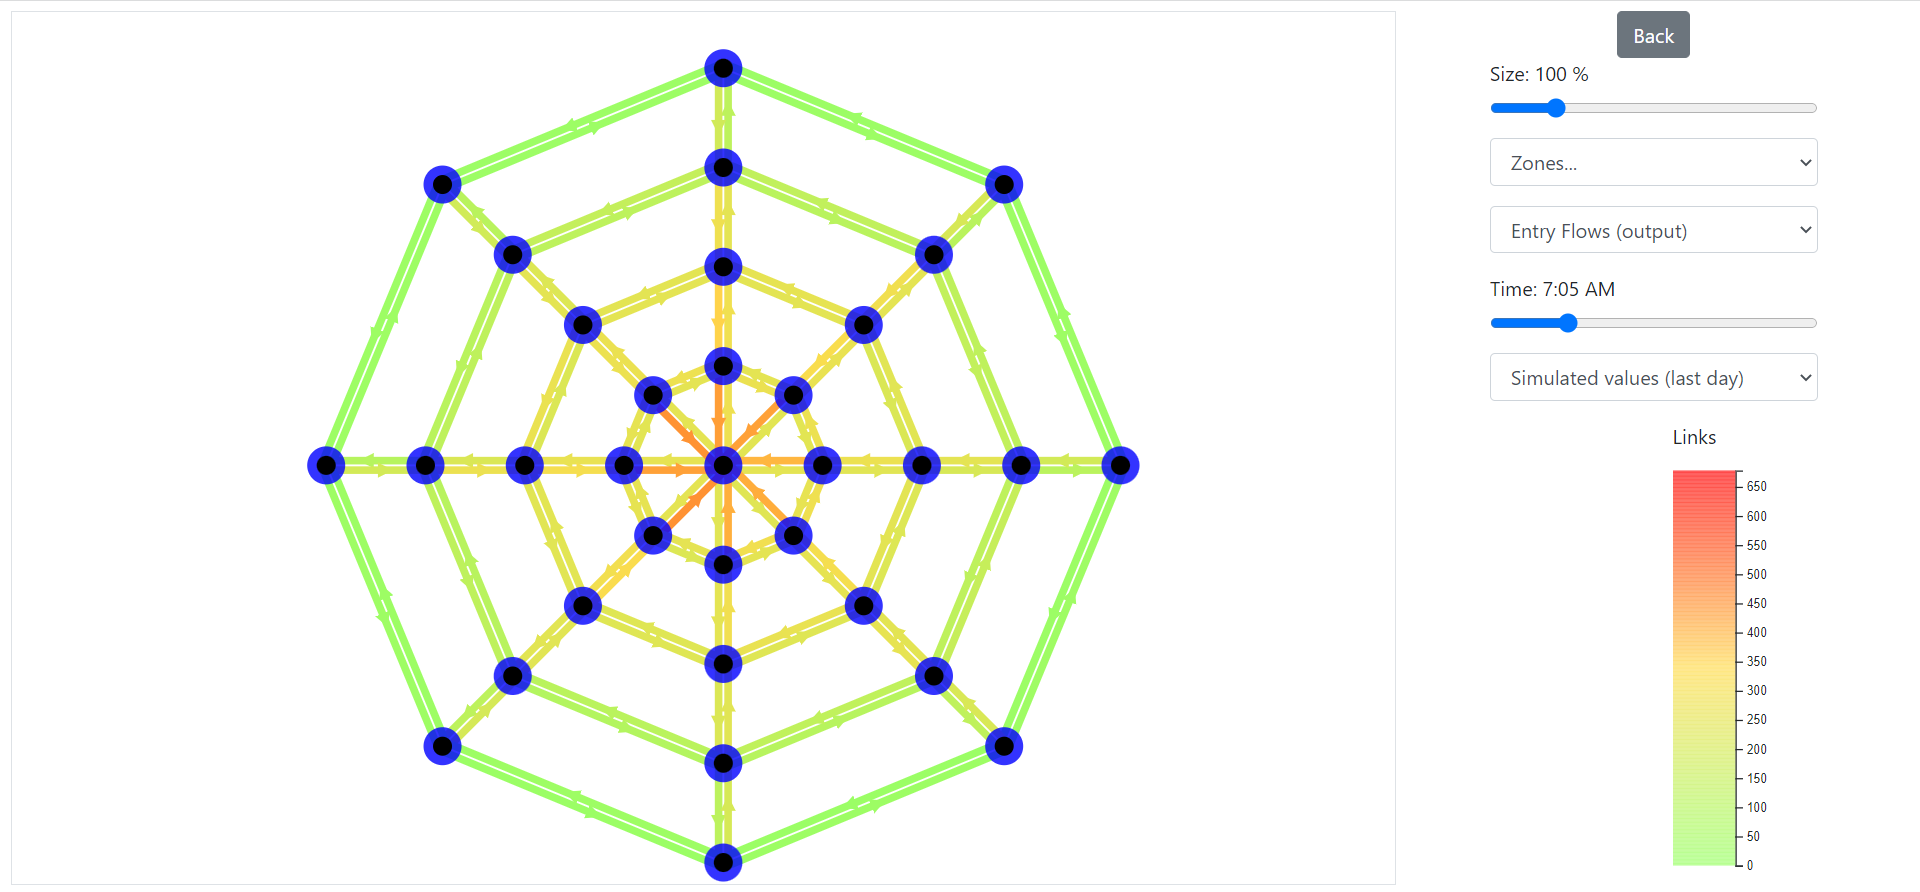
\includegraphics[width=1\textwidth]{Images/Step2/results_on_network_705am.png}
    \caption{Entry flows in the network at 7:05 am}
    \label{fig:Entry flows in the network at 7:05 am}
\end{figure}
\end{minipage}
\begin{minipage}[c]{0.5\textwidth}
\begin{figure}[H]
    \centering
    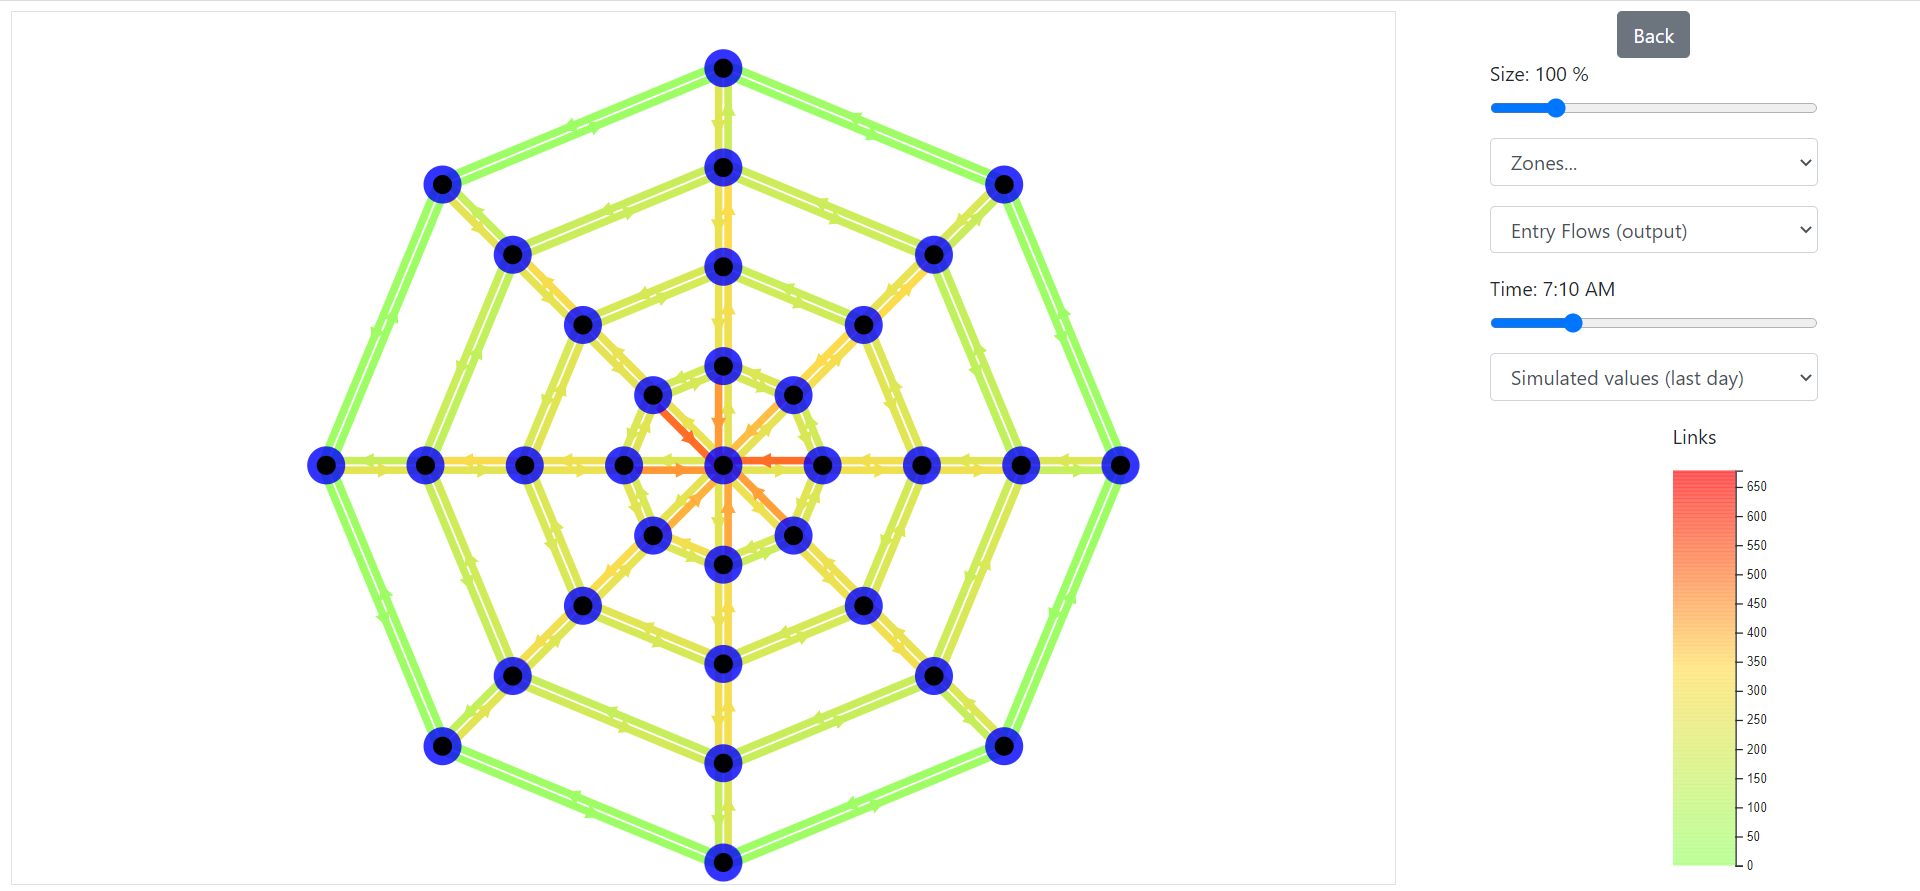
\includegraphics[width=1\textwidth]{Images/Step2/results_on_network_710am.png}
    \caption{Entry flows in the network at 7:10 am}
    \label{fig:Entry flows in the network at 7:10 am}
\end{figure}
\end{minipage}





\subsection{Convergence of the results}
\label{section:Convergence of the results}


On the basis of the graph representing congestion as a function of iterations (\ref{fig:Congestion percentage function of iterations (days)}) and that of speed and travel time as a function of iterations (\ref{fig:Speed and Travel time function of iterations (days)}), we can identify a point at which it is possible to consider that there is a convergence of the data.

First of all, we can see that in the very first iterations, the results obtained become less and less good. This is due to the initial calibration of the simulation parameters (at the beginning, the parameters are far from optimal and there is a short "trial and error" phase). After this initial phase, the results get better and better. Indeed, we notice that the proportion of congestion decreases from more than 70\% to about 35\%. The speed increases (from 33 [km/h] to 42 [km/h]) and the travel time decreases (from 42 [min] to less than 32 [min]). Finally, the values start to stagnate and it is from this point on wards that convergence between the different iterations (across the days of analysis) can be considered to have occurred. In our case, we can consider that there is convergence of the results from around iteration 40.

\begin{minipage}[c]{0.5\textwidth}
\begin{figure}[H]
    \centering
    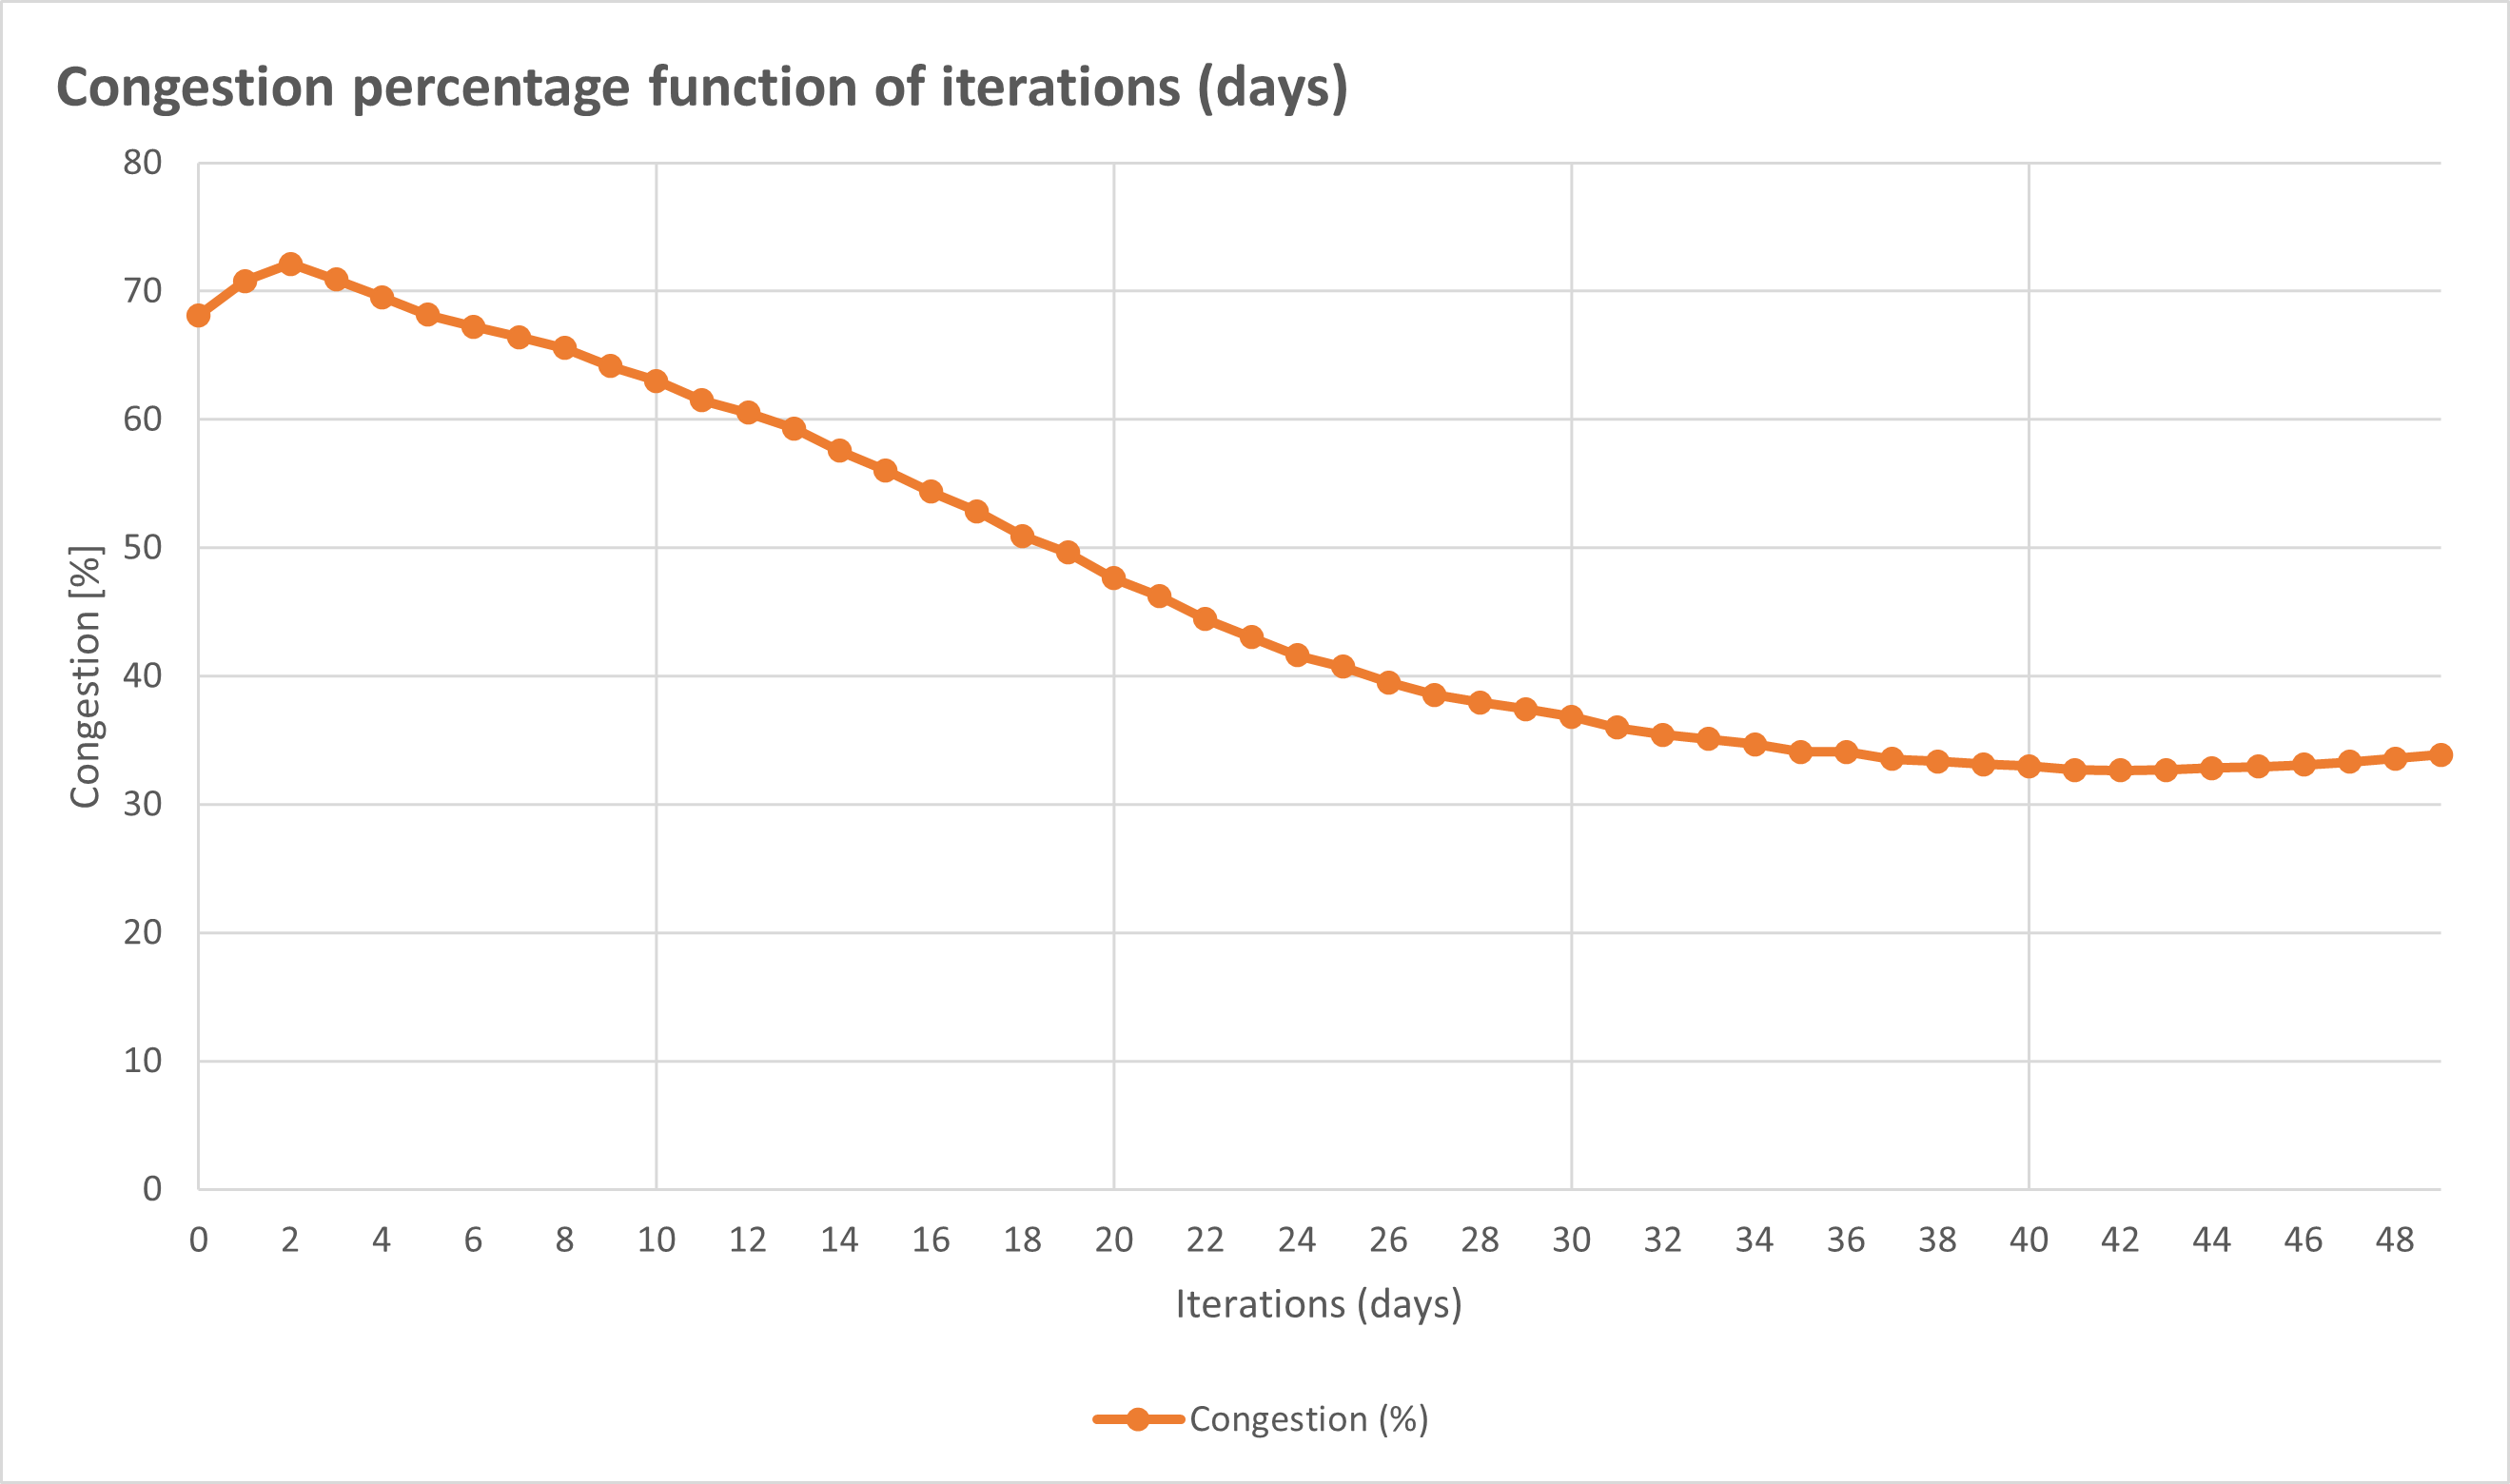
\includegraphics[width=1\textwidth]{Images/Step2/Congestion_percentage_function_iterations.png}
    \caption{Congestion percentage function of iterations (days)}
    \label{fig:Congestion percentage function of iterations (days)}
\end{figure}
\end{minipage}
\begin{minipage}[c]{0.5\textwidth}
\begin{figure}[H]
    \centering
    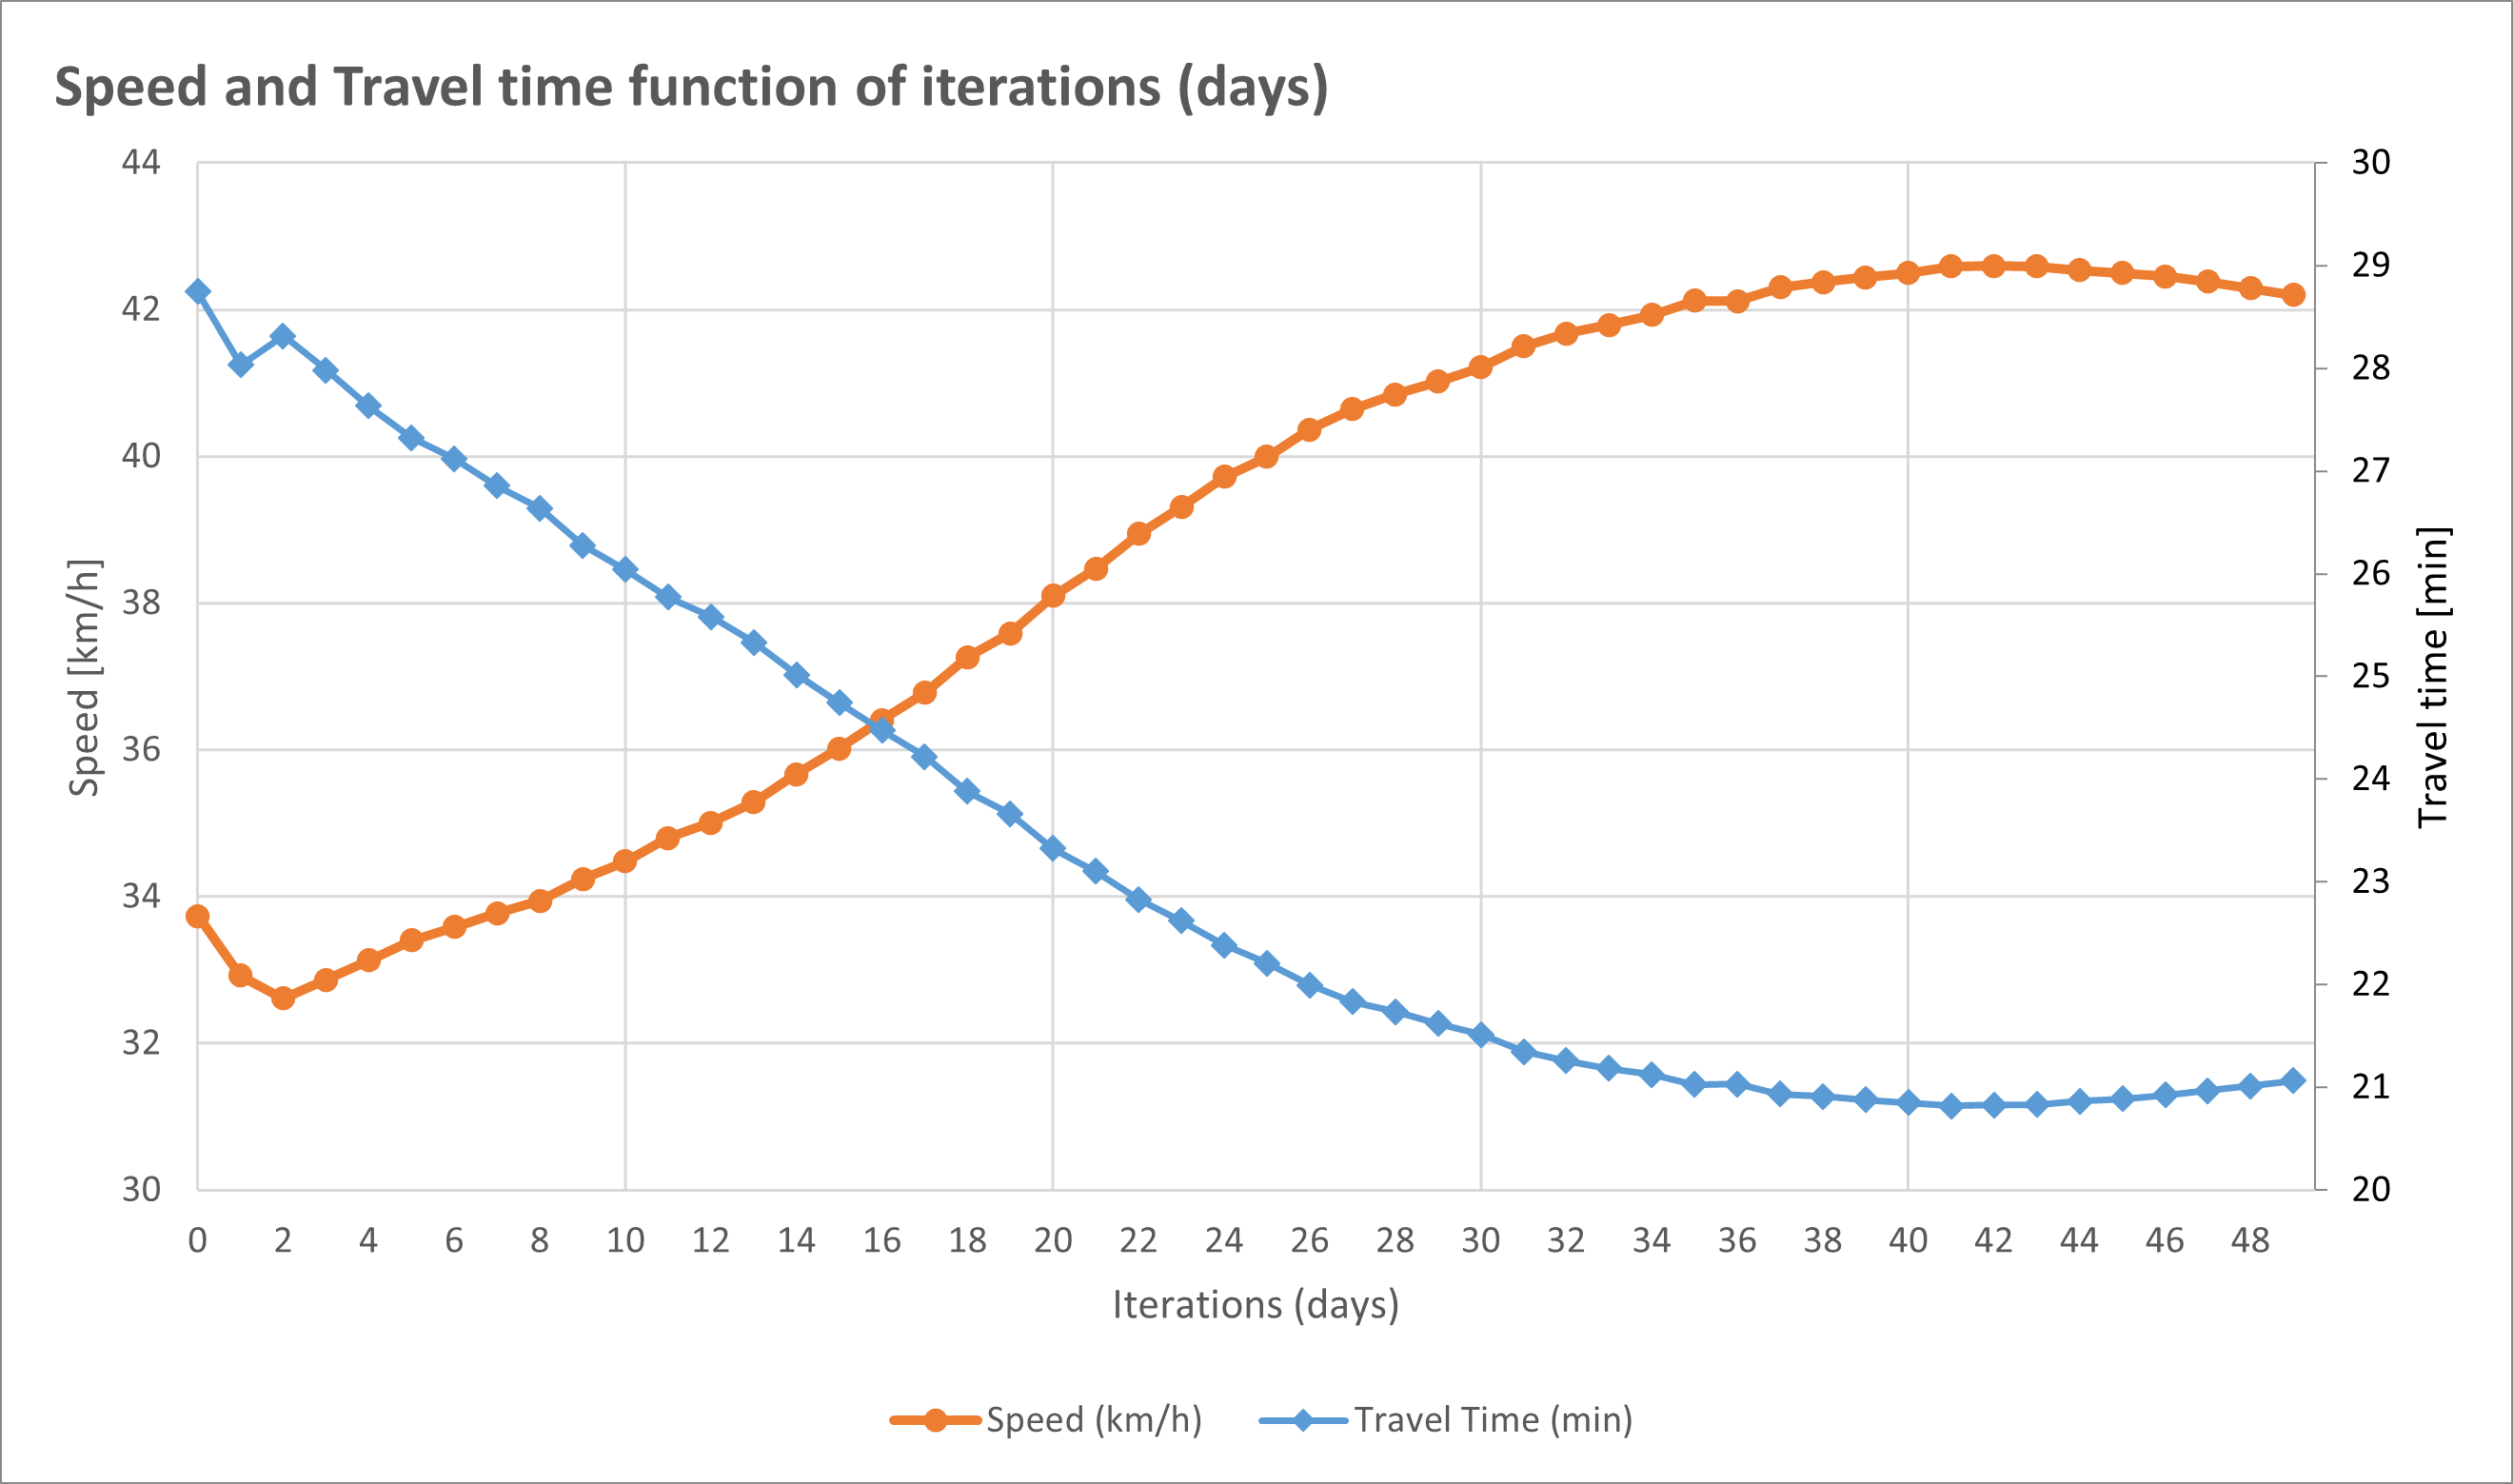
\includegraphics[width=1\textwidth]{Images/Step2/Speed_travel_time_function_iterations.png}
    \caption{Speed and Travel time function of iterations (days)}
    \label{fig:Speed and Travel time function of iterations (days)}
\end{figure}
\end{minipage}



\subsection{Early, on-time and late ratios analysis}
We can study the evolution of the early, on-time and late arrival rates thanks to the pie chart representing the evolution of these different rates as a function of time (\ref{fig:Ratios function of iterations (days)}).\\

First of all, we observe that during the first day of analysis, the late arrival rate is about 50\%, which is very high. This is understandable since all the users will behave the same way during this first iteration and thus strongly overload the network, which results in many delays. Following the learning model described in Formula 12, each traveller will try to reduce the total cost, part of which is the delay time.\\

Then, until iteration 21, the early arrival rate increases while the late arrival rate decreases and the on-time arrival rate increases slightly. From formula 13, it can be observed, during this phase, the main objective of the simulator is to decrease the late arrivals as much as possible because of the high penalty for arriving late, which increases early arrivals.\\

Finally, from iteration 25 onwards, when the proportion of late arrivals has stabilized (or increases very slightly), the proportion of early arrivals decreases, which leads to a greater increase in on-time arrivals. This will happen until about iteration 36. From this day until the end, the share of on-time arrivals will stabilize and it is the increase in late arrivals that will compensate for the decrease in early arrivals (but in a smaller proportion than the initial delay decrease), but this change is not significant, which is still a stabilize results. In the final situation, there are about 59\% early arrivals, 29\% on-time arrivals and 12\% late arrivals.\\

The behaviour of the simulator is perfectly logical. First, it will try to reduce the number of late arrivals (which is the worst situation). Consequently, the users will leave their homes much earlier and more diffusely. This will cause a drastic increase in early arrivals. However, during this operation, the proportion of on-time users will increase slightly. This is because a part of the users will leave slightly later from their homes, having experienced arrivals too early at their workplaces. Subsequently, this adaptive behaviour will gradually spread among the users, increasing on-time arrivals. Finally, as a result of this diffusion, the share of late arrivals will again increase slightly, as too many people start leaving too late. However, this will occur to a lesser extent than at the beginning. In the end, there are many more early arrivals than late arrivals, since it is less of a penalty to arrive early than late at work.

\begin{figure}[H]
    \centering
    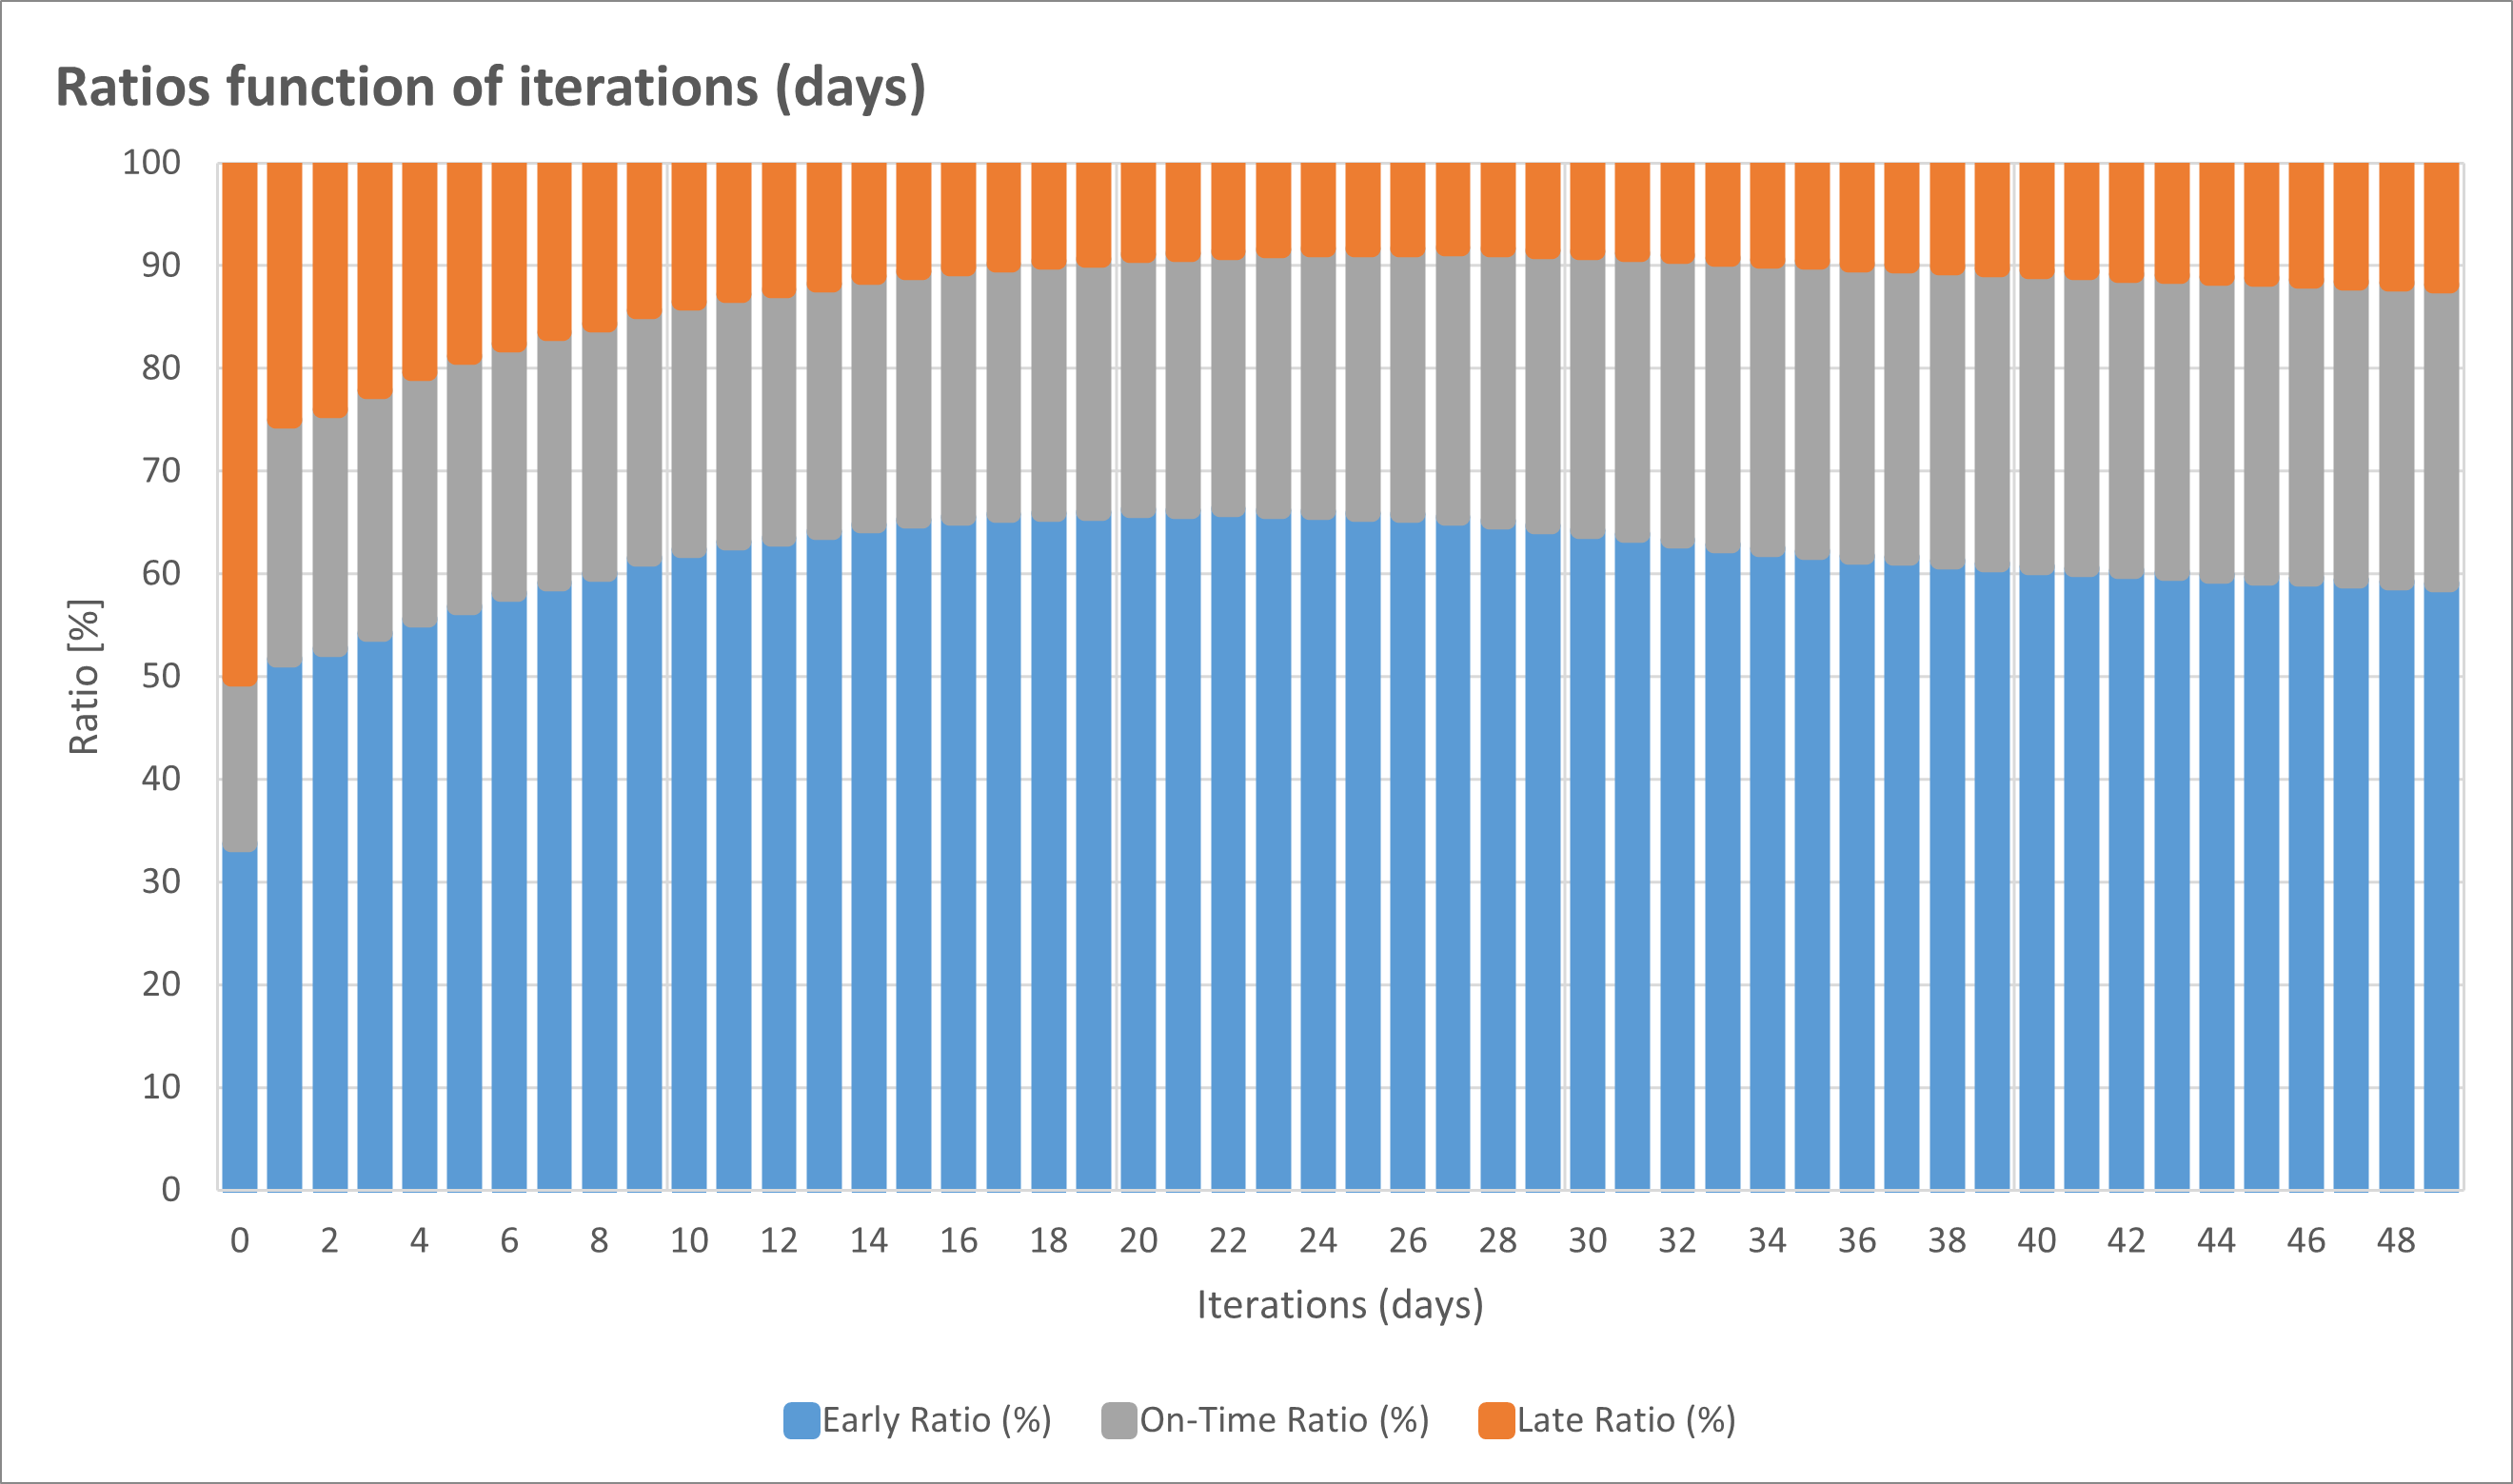
\includegraphics[width=0.8\textwidth]{Images/Step2/Ratios_function_iterations.png}
    \caption{Ratios function of iterations (days)}
    \label{fig:Ratios function of iterations (days)}
\end{figure}



\subsection{Changing user behaviour through experiential learning}

As mentioned in the section \ref{section:Convergence of the results}, the proportion of congestion decreases over time (except for the very first days of analysis). This is a consequence of a change in user behaviour. Indeed, the goal of the users is to have the lowest possible travel time while arriving neither early nor late. To reduce travel time, they need to avoid a congested situation that will cause them to experience a long travel time and, consequently, a possible delay to their workplace. Having a more diffused time distribution among users helps to reduce congestion upon their arrival in the downtown area and, consequently, to reduce their travel time.\\

It is now interesting to consider which change in behaviour has the greatest impact on reducing congestion. By definition, users can change three characteristics of their trip: departure time, mode choice and route choice. Thus, one of these three parameters has a greater effect on reducing congestion than the other two. In the following graph (\ref{fig:Normalized ratios function of iterations (days)}), we represent the variation of these three parameters concerning the initial state. We have therefore normalized these three quantities so that they take the unit value at the beginning of the simulation.\\

\begin{figure}[H]
    \centering
    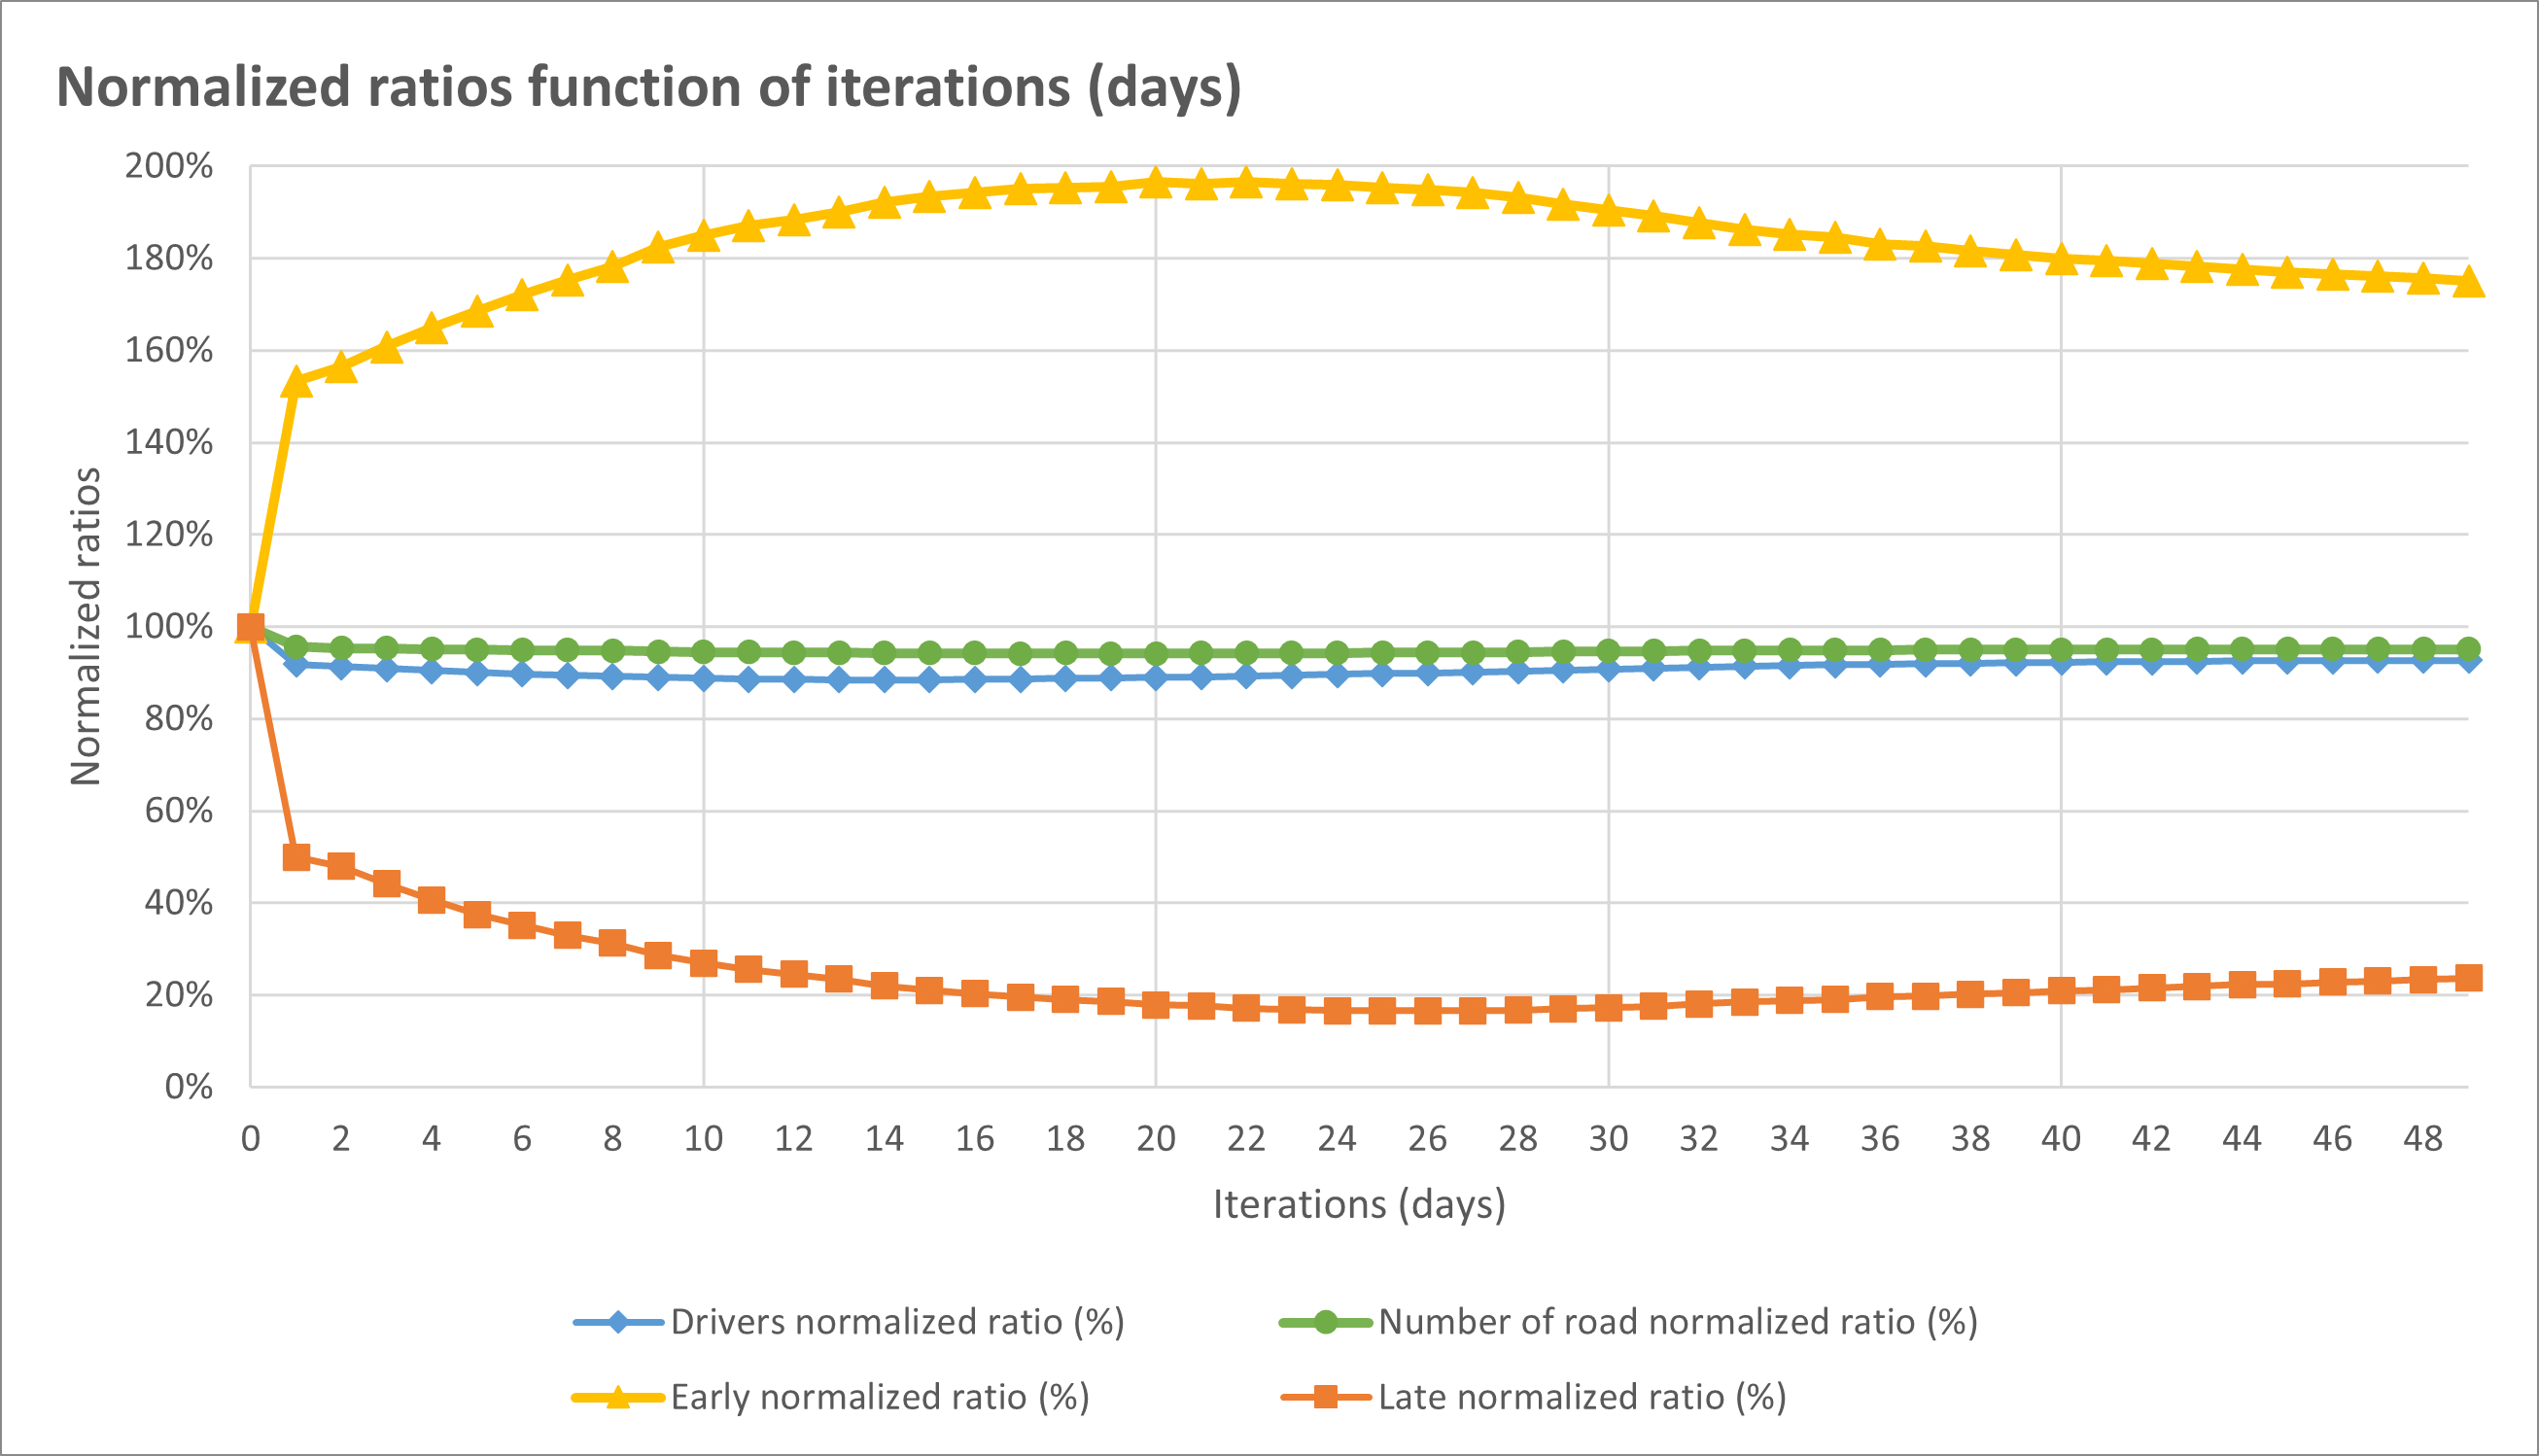
\includegraphics[width=0.8\textwidth]{Images/Step2/Normalized_ratios_function_iterations_2.png}
    \caption{Normalized ratios function of iterations (days)}
    \label{fig:Normalized ratios function of iterations (days)}
\end{figure}

We observe that the two most important variations, and to a much greater extent than for the other two parameters, are that of the early and late arrival, i.e. the choice of departure time. Indeed, these parameters vary by 75\% between the beginning and the end of the simulation for the "early" indicator and by 76\% for the "late" indicator, whereas the other two parameters vary by 5\% (route choice) and 7\% (mode choice). Intrinsically, the fact that this parameter (departure time) varies more than the others does not imply that it has the greatest impact on the variation in congestion.\\

%However, since the simulator varies the parameters to minimize congestion, it will vary the parameter that has the most impact. We can therefore consider that the parameter that changes the most is the one that has the greatest influence.\\ --> CETTE PARTIE ÉTAIT TOTALEMENT FAUSSE

However, we can deduce which parameter has the most influence by elimination. Indeed, as we have a variation in congestion, this must be explained by the variation of a parameter. Furthermore, we find that the variation of the indicators related to the modal choice and route choice parameters is very small if not practically zero. We can consider it negligible. Therefore, as these two types of parameters do not vary, they cannot cause congestion to vary. It is therefore the last type of parameter (departure time) that explains this evolution of congestion.\\

The fact that it is the departure time parameter that has the most influence is quite logical.\\
Indeed, when driving to the city centre, there is no time to wait for the bus. Therefore, it is more interesting to travel by car. We can see that the number of drivers decreases at the start when the situation is not good in terms of congestion. These users rely on public transport which is slightly more efficient. However, we do not know to what extent (existence of own site, public transport strategy, etc.). After the situation has eased, we observe that the number of drivers increases again. The variation of this parameter is therefore not essential.\\
The route choice parameter is not decisive since the network is perfectly symmetrical. There is no advantage for users to change the radial route to arrive at the city center.\\
The departure time parameter is therefore the most decisive.












\section{Task 3: Traveler Features}


Having analysed the data by considering only one type of traveller, we will now consider two different types of traveller:

\begin{itemize}

    \item Standard travellers,
    \item Low-income travellers

\end{itemize}

To do this, after downloading the original O-D matrix, we randomly split it into two sets of approximately equal size using Matlab code (see figure \ref{fig:Code Matlab for the randomly division of OD-matrix}). It is important to do this randomly so as to avoid strange results that might arise from just splitting the data in half. With this we were able to assign the newly created O-D matrices to the two new categories.

\begin{figure}[H]
    \centering
    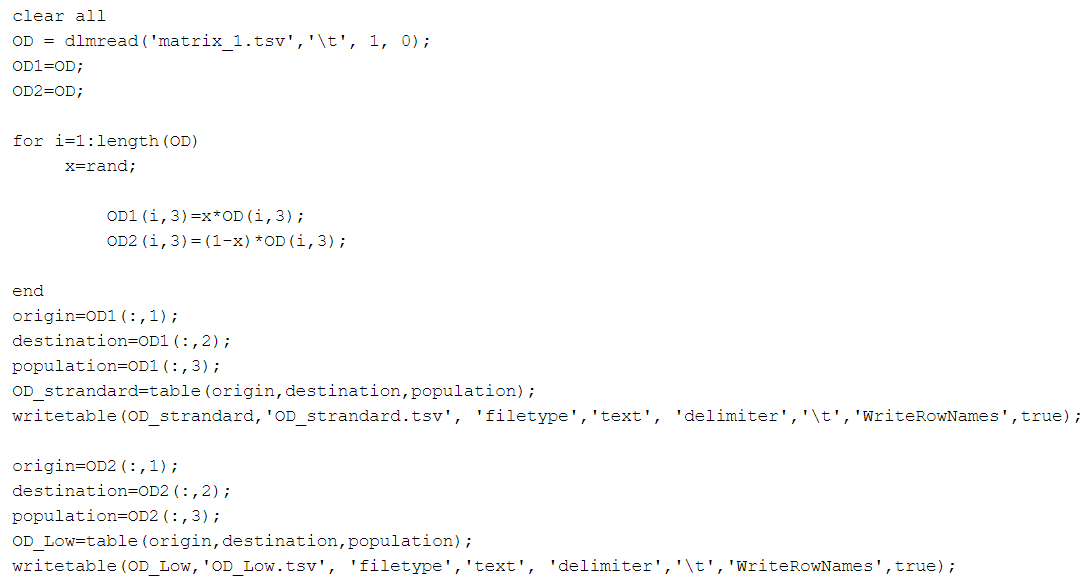
\includegraphics[width=1.0\textwidth]{Images/Step3/Code task 3.png}
    \caption{Code Matlab for the randomly division of OD-matrix}
    \label{fig:Code Matlab for the randomly division of OD-matrix}
\end{figure}

The code that has been created allows the original O-D matrix to be split into two O-D matrices as follows. For each origin-destination pair, we assign a random percentage of the population concerned to the new "Standard travellers" matrix and the remainder is assigned to the "Low-income travellers" matrix. For example, if we have for the O-D "A-B" 100 travellers initially, we assign a random percentage (e.g. 60\%) to the "Standard travellers" matrix (in this case, 60 travellers) and the rest (40\%, i.e. 40 travellers) to the "Low-income travellers" matrix.\\

The advantage of this allocation method (as opposed to just mixing the O-Ds and selecting half for one category and half for the other category) is that it appears more realistic in what it represents. Indeed, in the alternative method, we have a too clear (unnatural) distribution in the O-D. For example, we would have the entirety of the people doing the "A-C" trip in one category (e.g. low-income). This is problematic because it is unlikely that all people making the same trip would be in a single socio-economic category.\\

This could be seen as an advantage as it would create neighbourhoods (living and working) with a single socio-economic bracket. However, this is not the case as it is quite possible that people making the "A-B" trip are in one category and those making the "A-C" trip in another. Just as it is highly likely that it is the same for the destination ("A-C" different from "B-C"). Therefore, the only potential advantage of this method is actually not an advantage and even a disadvantage since it divides the population too roughly, unlike the chosen method which divides the population by a random percentage. For this reason, we have kept this method.\\

It is important to note that we introduced a scaling factor in order to obtain a total number of travellers similar to the one observed in Task 2. We then set the same factor as in Task 2, namely 14.7067016. This gives us 130'203 standard travellers and 133'811 low-income travellers. The sum of the two categories (264'014) is equal to the total number of travellers in Task 2 (264'014). Moreover, each category represents about half of the travellers (to the nearest 0.7\%).

%This method of distributing O-D according to socio-economic profiles seems to us to correspond perfectly to a real situation. Indeed, in such a situation, it would be rather expected to observe differentiated origins according to the categories of travellers (people do not live in the same place according to their income).

\subsection{Differentiated parameter between standard and low-income travelers}
\begin{table}[]
    \centering
    \begin{tabular}{c|c}
        Name & Value \\
        \hline
        Number of traveller, $N$& 133811\\
        The value of the departure time $\mu$ & 2\\
        On-time window, $\delta$ & 10\\
        The value of time for public transportation & 10\\
        The value of time while driving, $\alpha$ & 10\\
        The early-arrival penalty, $\beta$ & 6\\
        The late-arrival penalty, $\gamma$ & 25\\
        Learning rate $\lambda$ & 0.1\\
        
    \end{tabular}
    \caption{The parameters table of task 3 simulation (low-income travellers)}
    \label{tab:The parameters table of task 3 simulation (low-income travellers)}
\end{table}
\begin{table}[]
    \centering
    \begin{tabular}{c|c}
        Name & Value \\
        \hline
        Number of traveller, $N$& 130203\\
        The value of the departure time $\mu$ & 2\\
        On-time window, $\delta$ & 10\\
        The value of time for public transportation & 15\\
        The value of time while driving, $\alpha$ & 10\\
        The early-arrival penalty, $\beta$ & 6\\
        The late-arrival penalty, $\gamma$ & 25\\
        Learning rate $\lambda$ & 0.1\\
        
    \end{tabular}
    \caption{The parameters table of task 3 simulation (standard travellers)}
    \label{tab:The parameters table of task 3 simulation (standard travellers)}
\end{table}
The parameter that is expected to differ between low-income and standard travellers is the value of time on public transport. Indeed, the main parameters that may vary are the penalties for being early or late, the value of time on public transport, and the value of time by car.\\

The parameters related to penalties could vary according to the socio-economic profile. However, it is difficult to determine in which direction this difference would occur, or even whether there is any real variation between the two profiles.\\

The parameter of the cost of car travel might be higher for low-income travellers. In fact, it is mainly the difference between the cost of car travel and public transport that should be lower for low-income people than for high-income people. This is because people with higher incomes will prefer a more efficient and comfortable mode of transport, even if it is more expensive. For them, the value of time on public transport will therefore be much higher than that in a car. For low-income people, it seems logical that the difference between the two modes will be smaller or even zero since they will value comfort less than price.\\

Thus, it is possible to either increase the value of time spent by car for low-income people or decrease the value of time spent by public transport for low-income people. Since it makes more sense for high-income people to have the same or higher value of time, we decide to decrease the value of time on public transport for low-income people. Moreover, decreasing the value of time by 5 leads to the same value of time spent by car and public transport for low-income people. This seems consistent since the choice of transport mode is less important for them (comfort is not taken into account).\\

Finally, it should be noted that we could have changed the penalty for public transport rather than the value of time on public transport. However, a priori, the willingness (or unwillingness) to use public transport can be considered equivalent for any type of user. On the other hand, the lack of comfort and use of public transport during the journey may be more acceptable to a low-income person than to a high-income person. This is an assumption that we will consider in the following.

\subsection{Congestion results between one type of traveller and two types (low-income and standard)}

Based on this parameter change, we ran our code with both types of travellers. This allowed us to obtain a graph of the evolution of the congestion according to the iterations (days of the study). Moreover, we also represented on the same graph the evolution of the congestion in the case of Task 2 (with one type of traveller). 

\begin{figure}[H]
    \centering
    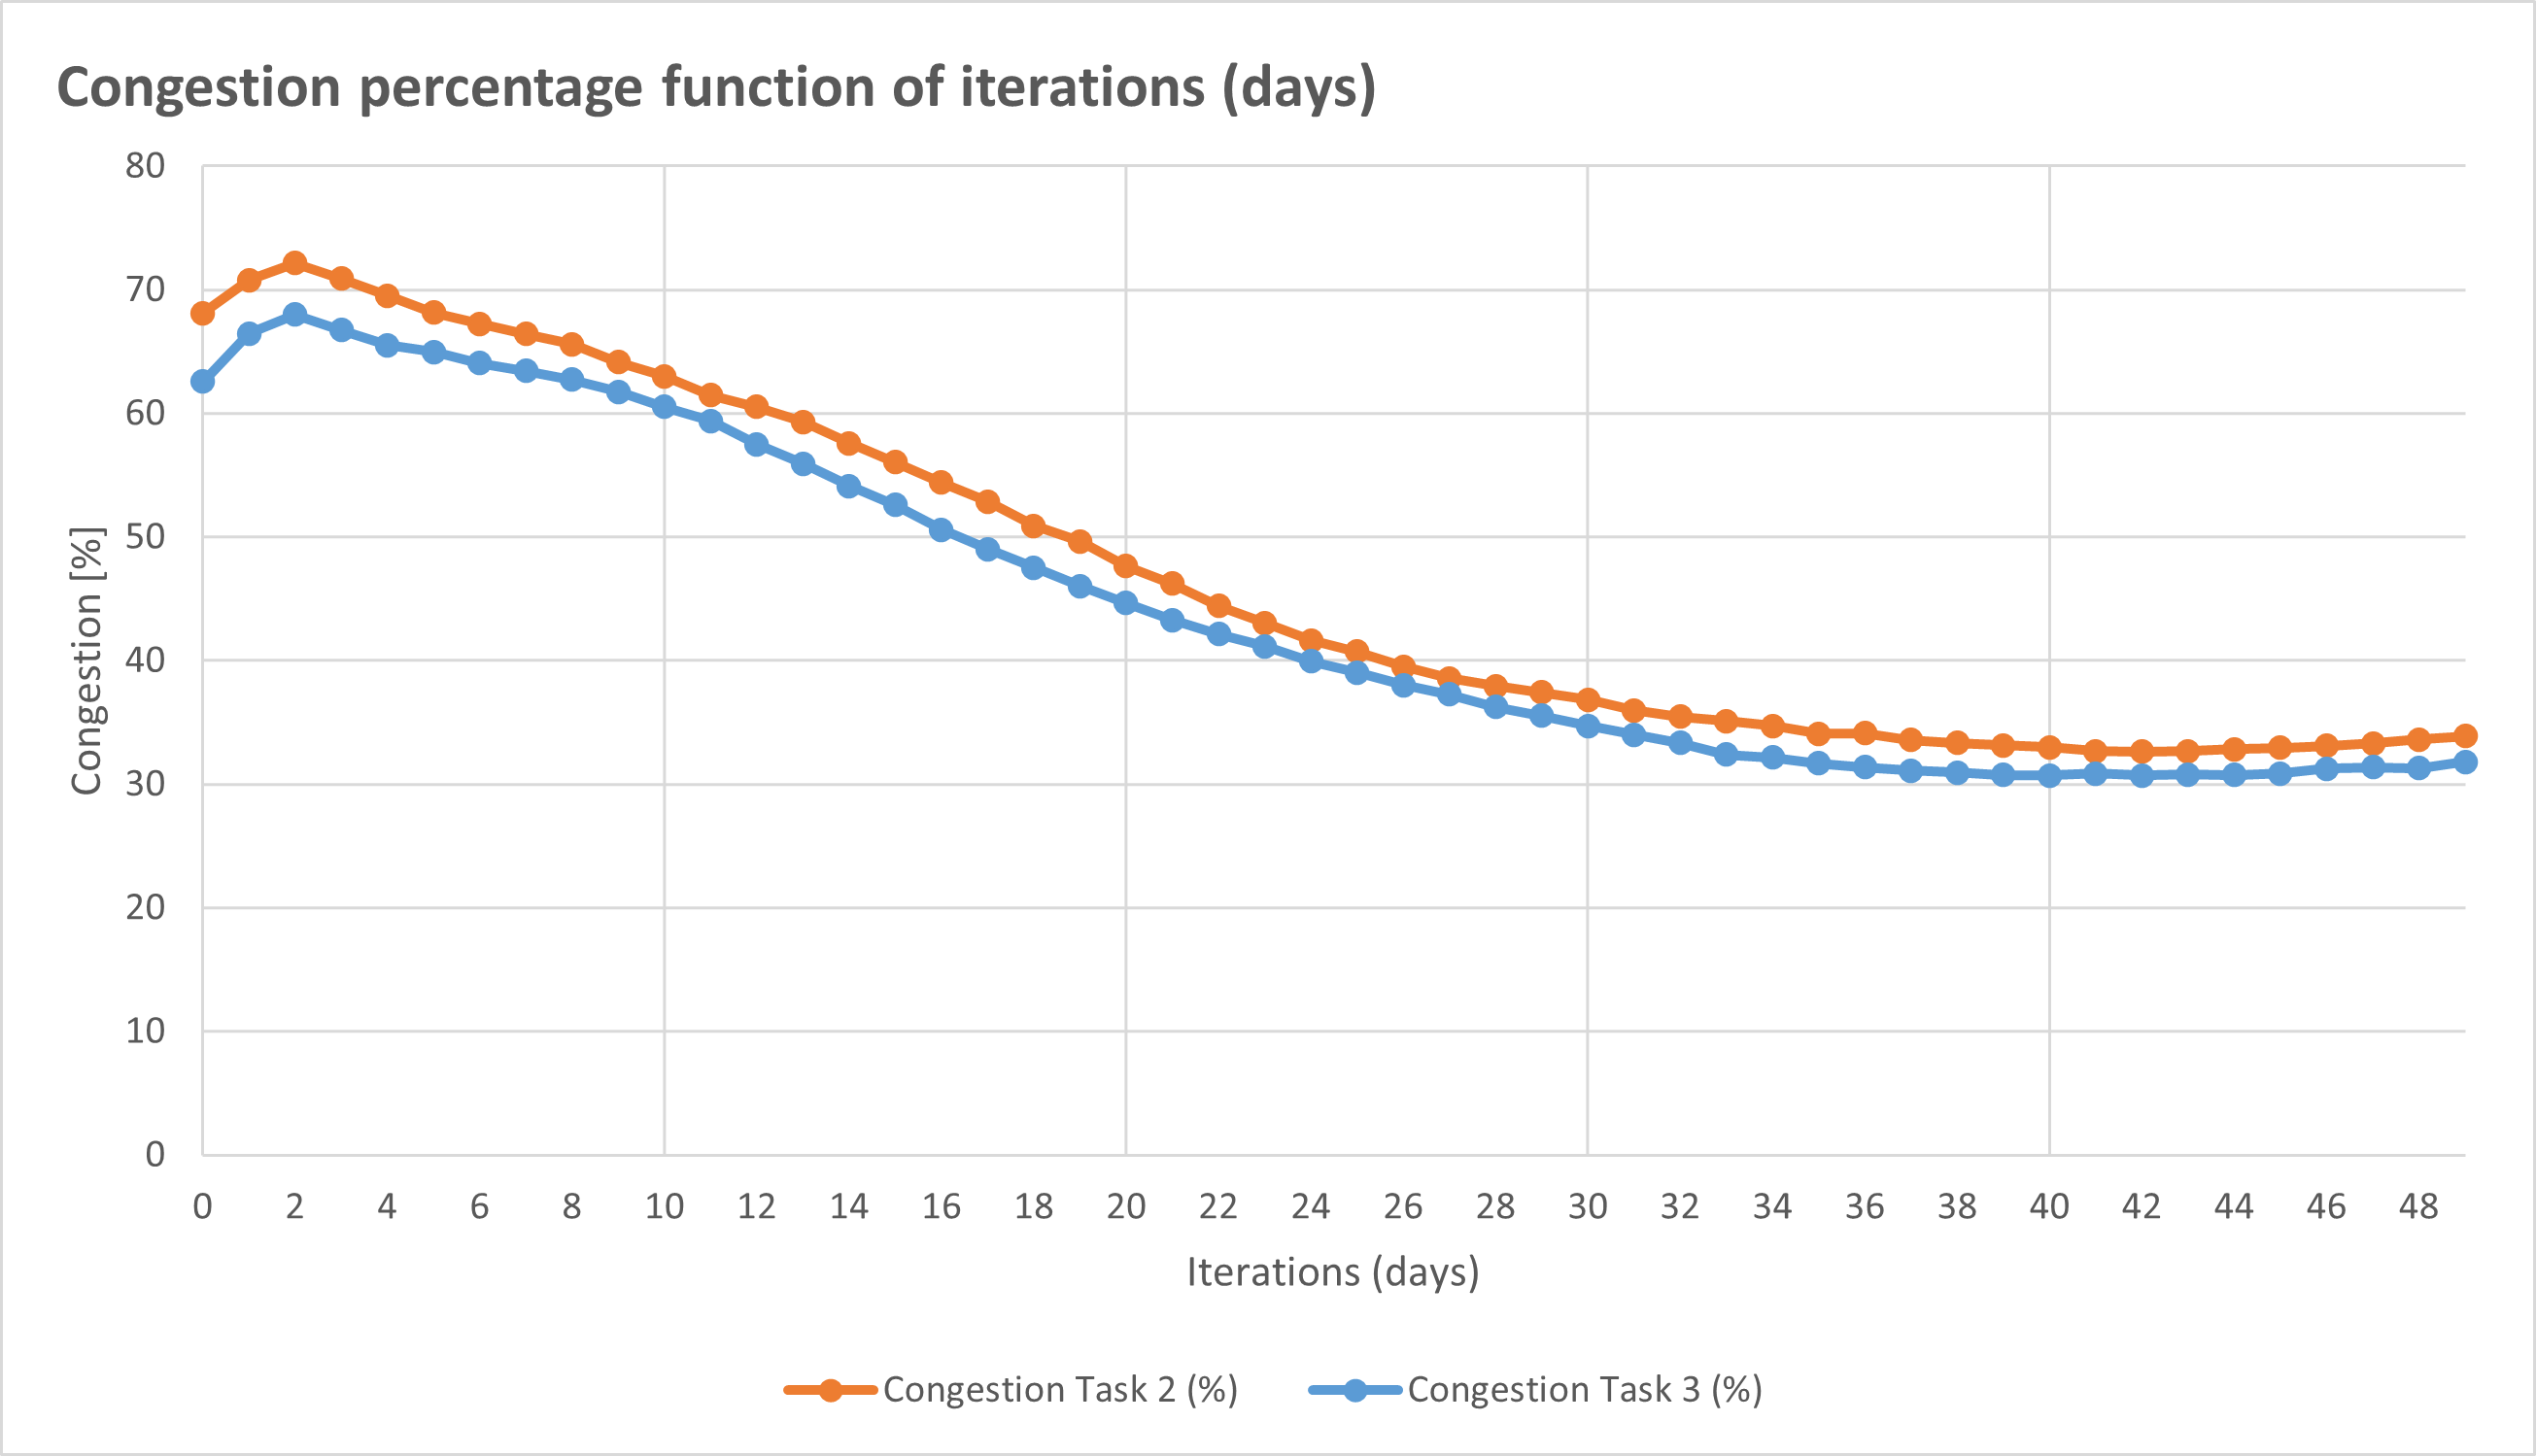
\includegraphics[width=0.8\textwidth]{Images/Step3/Congestion_percentage_function_iterations.png}
    \caption{Congestion percentage function of iterations (days)}
    \label{fig:Congestion percentage function of iterations (days)}
\end{figure}

Moreover, in order to study the impact of this categorization with respect to Task 2, we produced a graph representing the consumer surplus as a function of the iterations.

\begin{figure}[H]
    \centering
    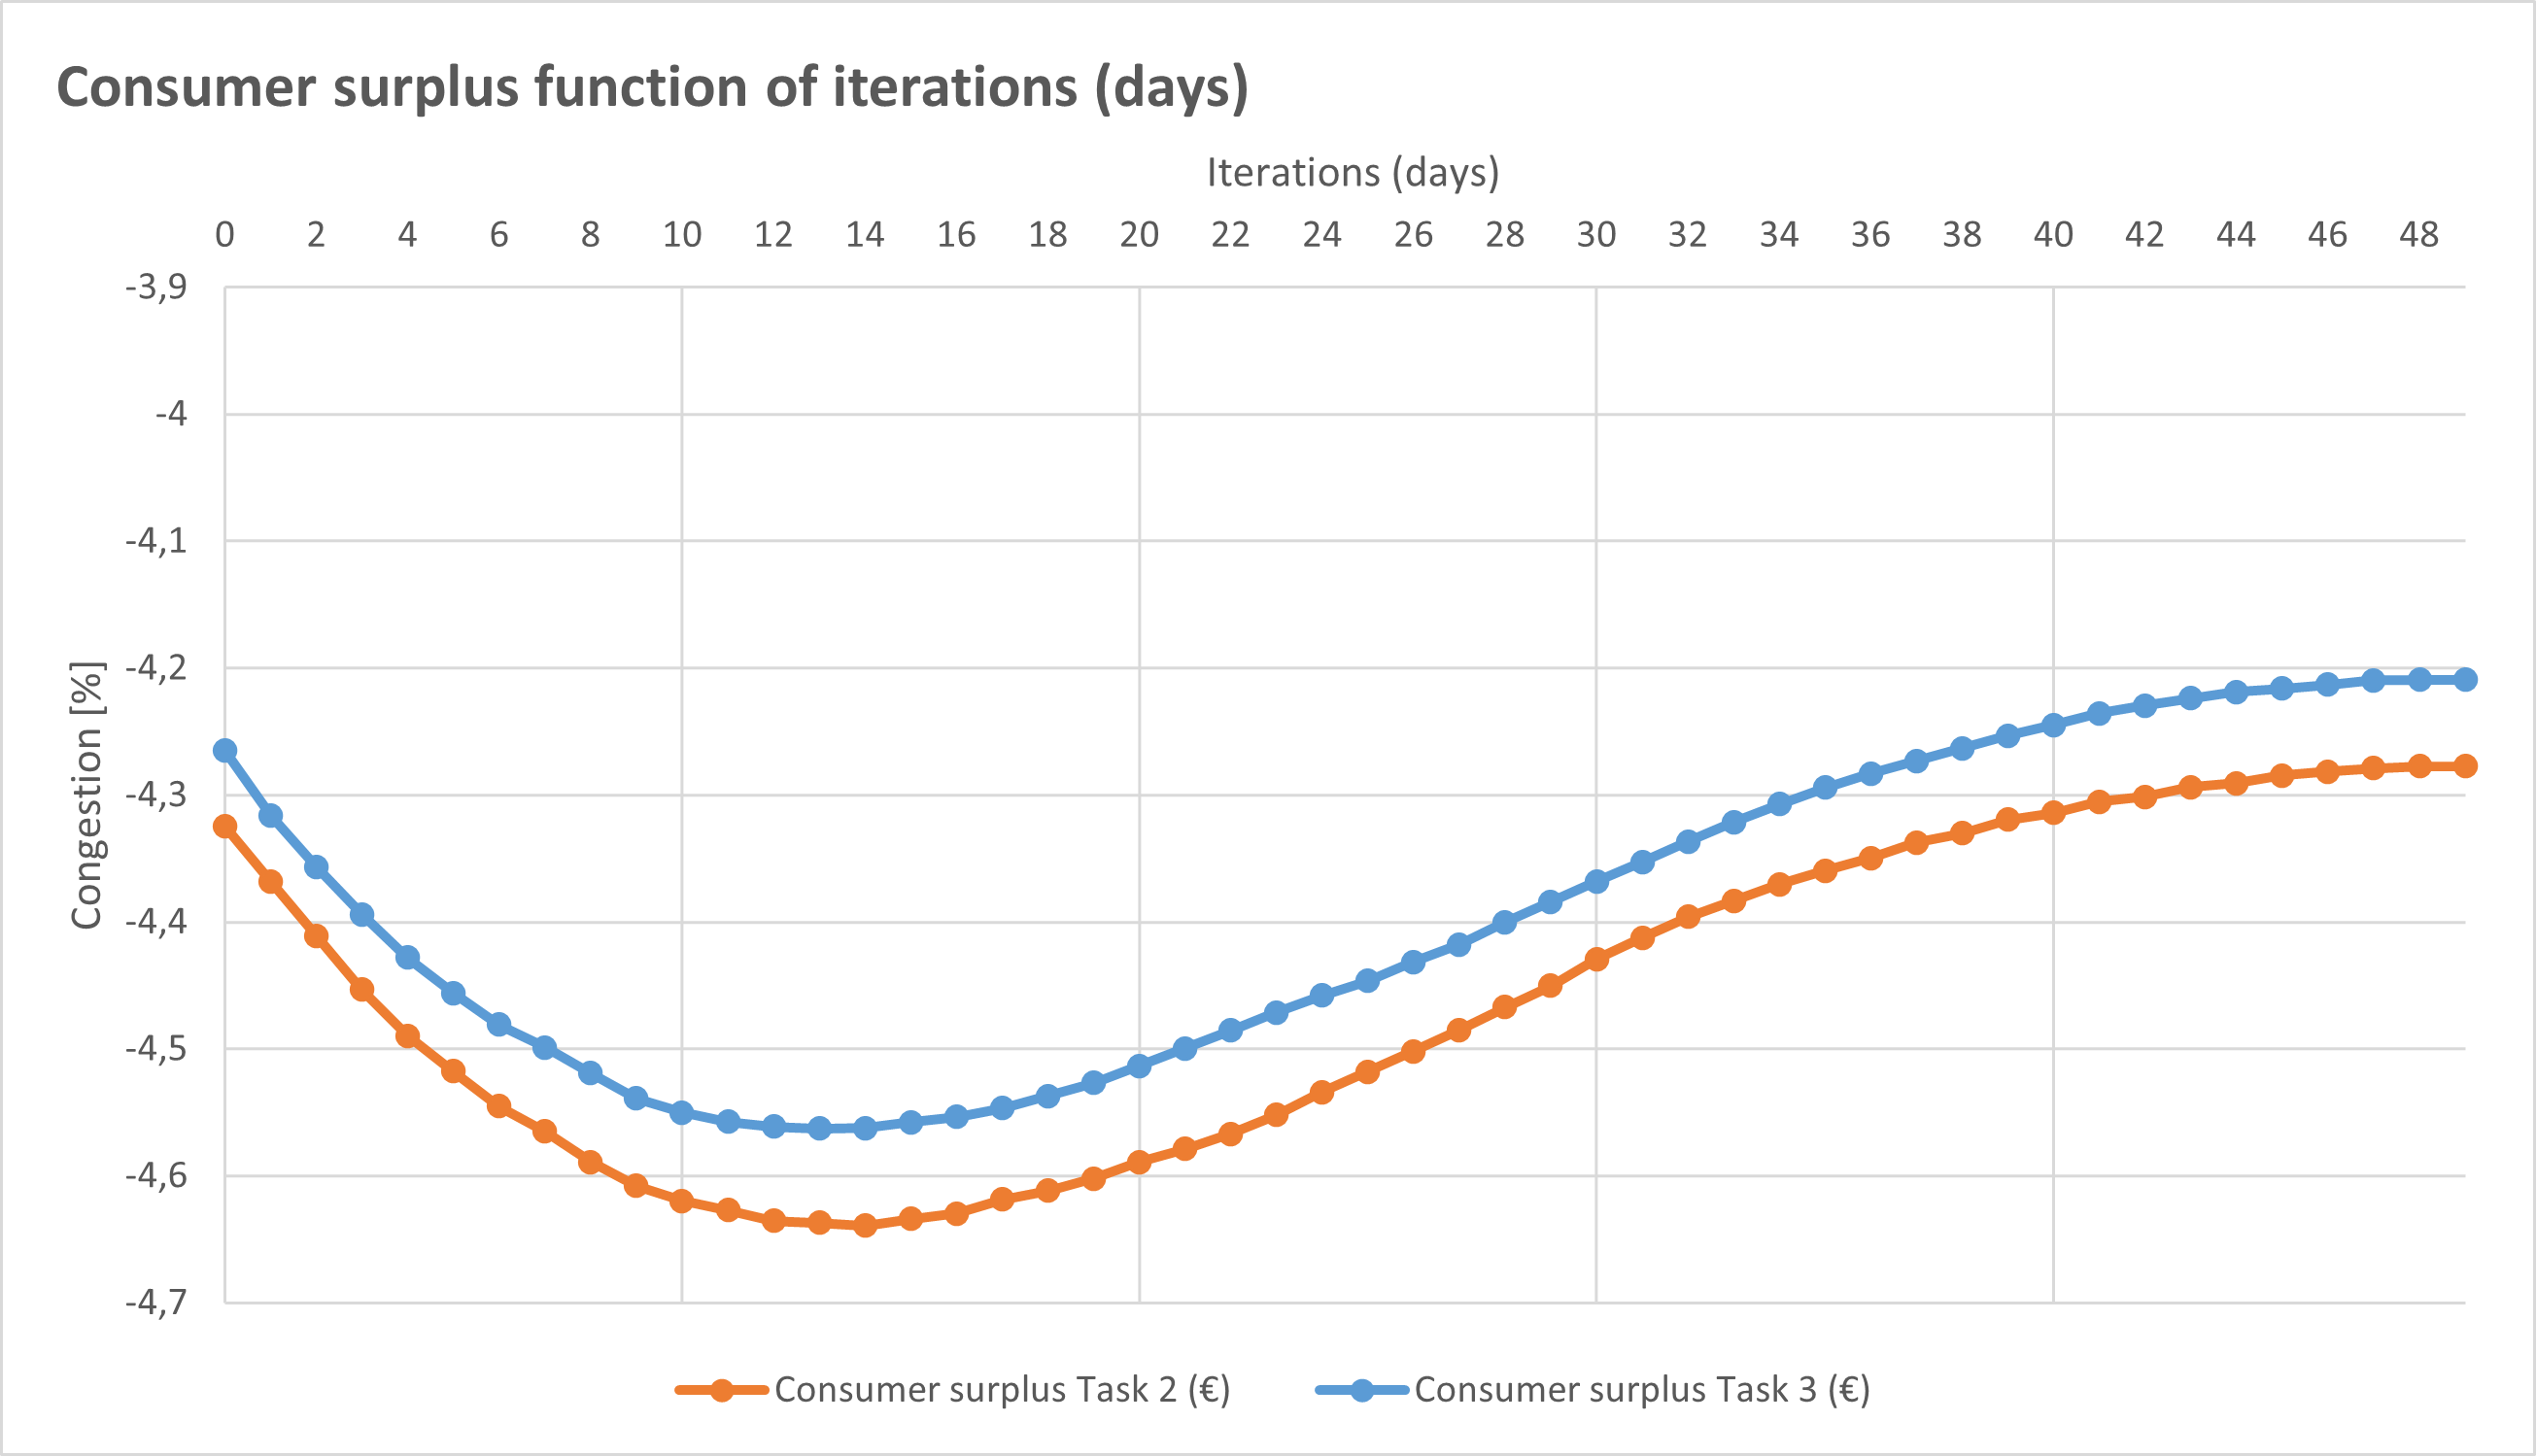
\includegraphics[width=0.8\textwidth]{Images/Step3/Consumer_surplus_function_iterations.png}
    \caption{Consumer surplus function of iterations (days)}
    \label{fig:Consumer surplus function of iterations (days)}
\end{figure}


\subsection{Analysis of the differences in results}

First, we look at the difference in the evolution of congestion in the two study cases. We find that congestion is relatively lower when the two socio-economic categories are distinguished than when only one category is considered. However, we note that the general trend follows that of the first curve. We will try to explain this.\\

%Furthermore, we see that the evolution of congestion is lower in the case of both categories than in the case of a single category. This is explained by the fact that since the situation is initially (in the first iterations) better in the case of differentiated categories, the improvement of the situation can only be more limited.\\

We can first question why this slight improvement from the beginning of the iterations in the differentiated case. We find that the total number of drivers is lower in the differentiated case than in the other. This makes sense, since the value of time is lower for low-income travellers, and they are more likely to use public transportation. As a result, there will be fewer vehicles on the system, which will reduce congestion. Next, we can comment on a similar development as before. The improvement in congestion will be of a similar magnitude, since, although there will be people who do not drive, there will still be a large proportion (a large proportion of the standard and a proportion of the low-income) who do. As the iterations proceed, this number will decrease, due rather to changes in their departure time behaviour (as explained above).\\

Second, we can look at the difference in consumer surplus in these two cases.\\

The consumer surplus represents the consumer's 'gain' compared to the situation that the consumer considers neutral (neither favourable nor unfavourable). In these simulations, the consumer surplus will always be smaller than zero, i.e. unfavourable for the traveller. The aim is to get as close as possible to zero to arrive at the neutral situation.\\

We observe that between the situation with one category of travellers and the situation with two types of travellers, we have a consumer surplus that is higher (closer to zero) in the second case. Thus, the situation is more favourable than the first one for travellers.\\

Indeed, by decreasing the value of time parameter in public transport for low-income people, more people will use this mode of transport and therefore fewer people will use the car. Consequently, as there will be fewer vehicles on the network, there will be less congestion and therefore fewer late or early arrival. This allows for a greater consumer surplus. The situation is therefore very beneficial for users.\\


\section{Task 4: Road pricing policy}
The Metropolis program makes it easy to implement road pricing policies by indicating the pricing and the period over which it takes effect.\\

In this last question, we will evaluate the effects of implementing different road pricing policies based on a single traveller profile (as in Task 2).\\

\subsection{Implementation of the constant road pricing policy}
First, we will analyse the results of a road pricing policy based on a constant toll of 2 between the beginning of the simulation day and 7:15 am. After this time, no toll is charged (as in Task 2). Note also that this pricing applies only to links between the inner ring road and the city centre.

\subsubsection{Results on the network}

We can now comment on the results obtained on the network and how congestion propagates in the network as a function of time in the morning.\\

Firstly, before 7:00 am, the network is not very congested. Secondly, at 7:00 am, flows form on the axes leading to the centre of the network, between belts 2 and 3. This corresponds to people leaving their homes to go to work in the city centre. If we compare with Task 2, we can see that this configuration took place at 6:45 am, i.e. 15 minutes earlier. Moreover, the flows entering the centre of the network are much lower than in Task 2, even at 6:45 am. This shows two things. The first is that the flows occur later in the morning. We will come back to this later. The second thing is that few people enter the city centre at 7:00 am because there is still the toll to pay. Therefore, the flows are low.\\

Then, the radial flows intensify and get closer to the city centre between 7:05 am and 7:10 am. This makes sense as the flow of vehicles will move from the periphery to the centre and at each ring, there will be more people (hence the intensification). However, although the flows in the city centre are increasing, they remain at a much lower intensity than those outside the first central ring.\\

Everything changes at 7:15 am. We observe then that the flows inside the city centre are very important (and even much more important than those observed in Task 2) and that they last from 7:15 am to 7:25 am (lower peak duration but higher intensity than in Task 2). Finally, the situation stabilises around 7:30 am.\\

\begin{minipage}[c]{0.5\textwidth}
\begin{figure}[H]
    \centering
    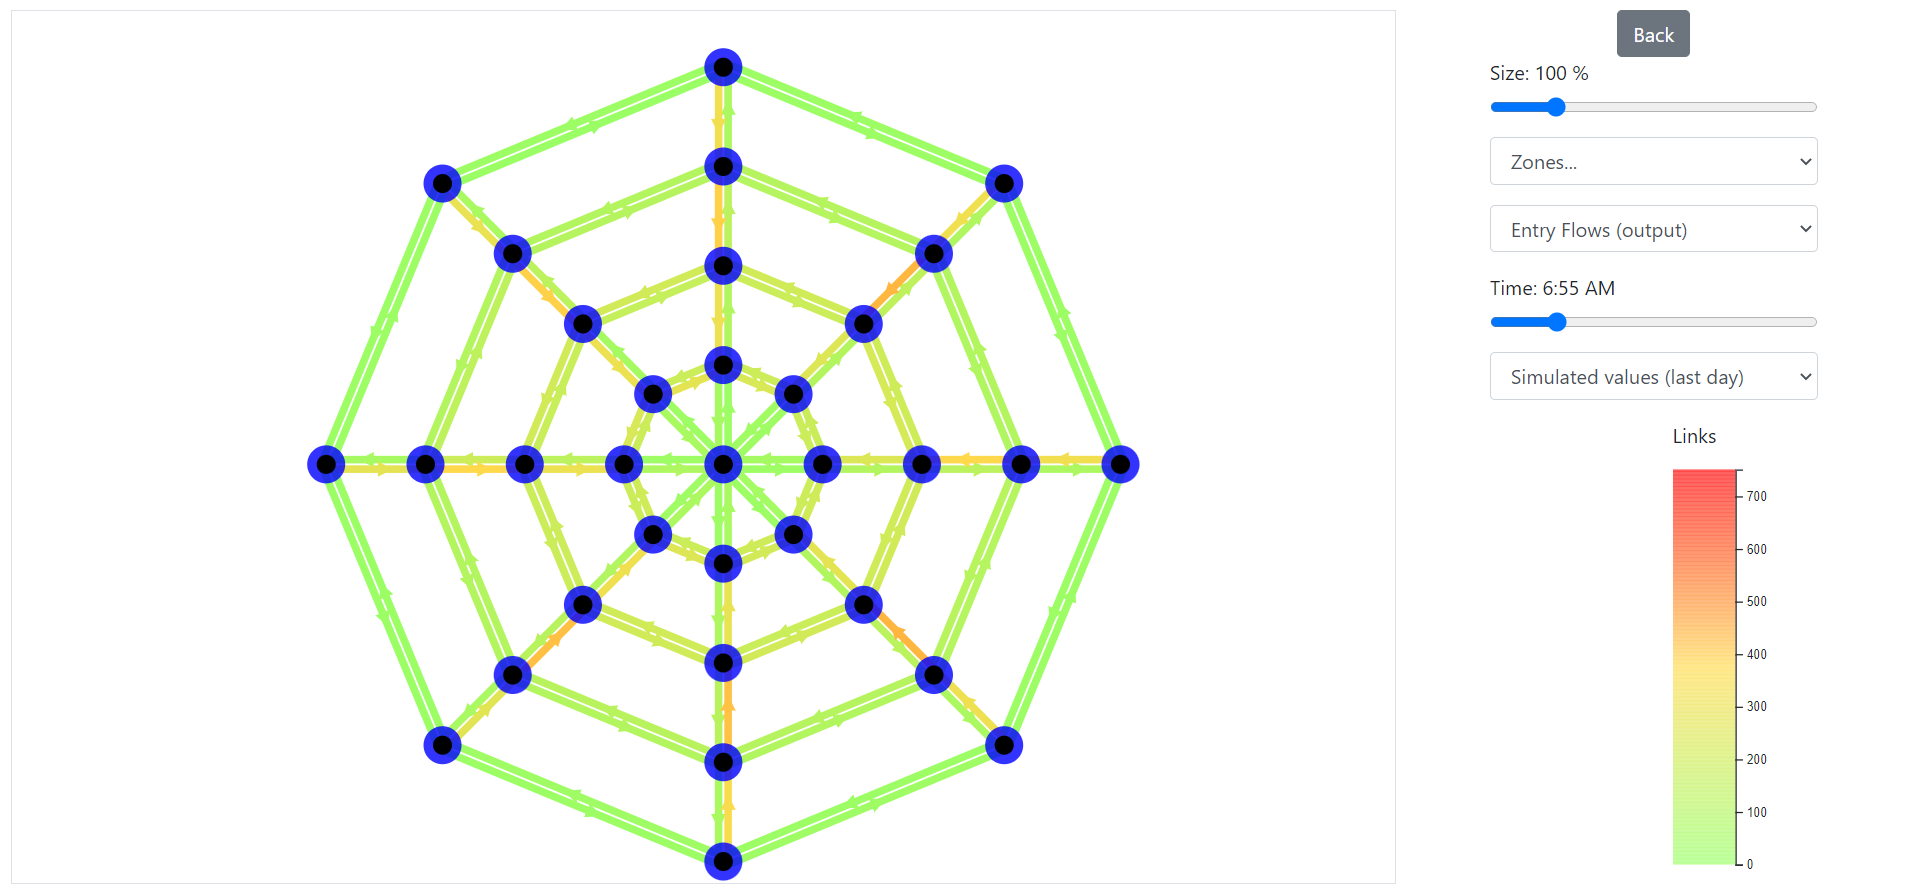
\includegraphics[width=1\textwidth]{Images/Step4/results_on_network__task4.1_655am.png}
    \caption{Entry flows in the network at 6:55 am with constant toll (Task 4.1)}
    \label{fig:Entry flows in the network at 6:55 am with constant toll (Task 4.1)}
\end{figure}
\end{minipage}
\begin{minipage}[c]{0.5\textwidth}
\begin{figure}[H]
    \centering
    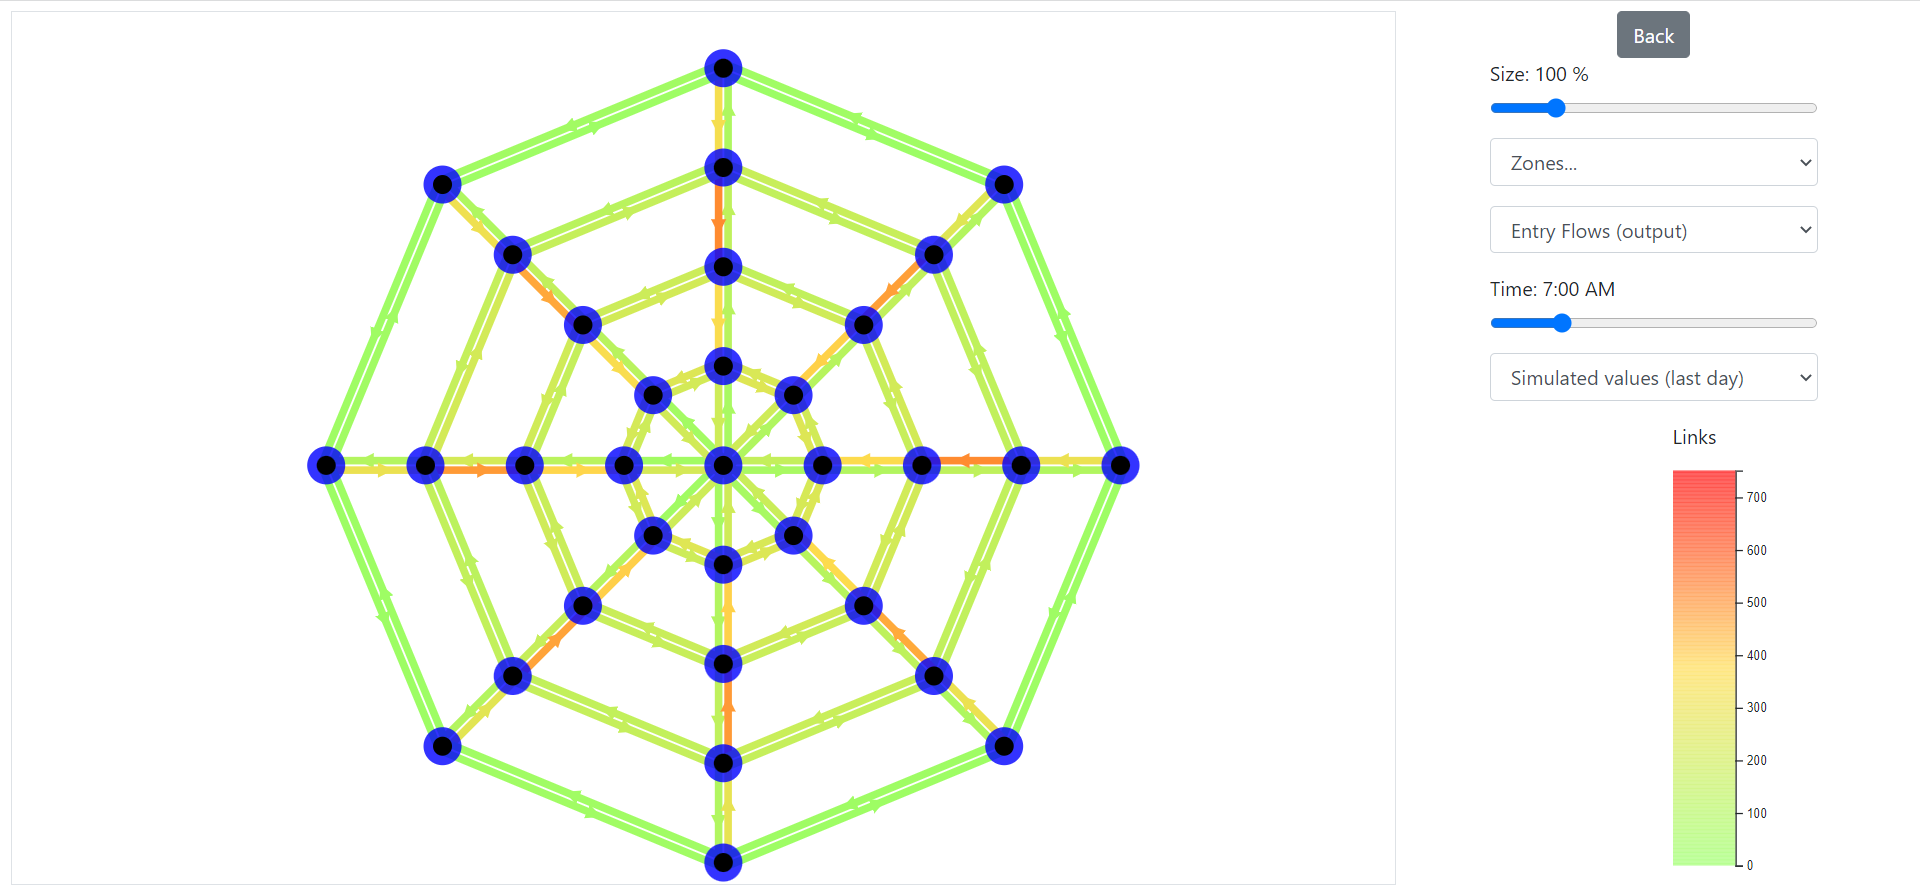
\includegraphics[width=1\textwidth]{Images/Step4/results_on_network__task4.1_700am.png}
    \caption{Entry flows in the network at 7:00 am with constant toll (Task 4.1)}
    \label{fig:Entry flows in the network at 7:00 am with constant toll (Task 4.1)}
\end{figure}
\end{minipage}
\begin{minipage}[c]{0.5\textwidth}
\begin{figure}[H]
    \centering
    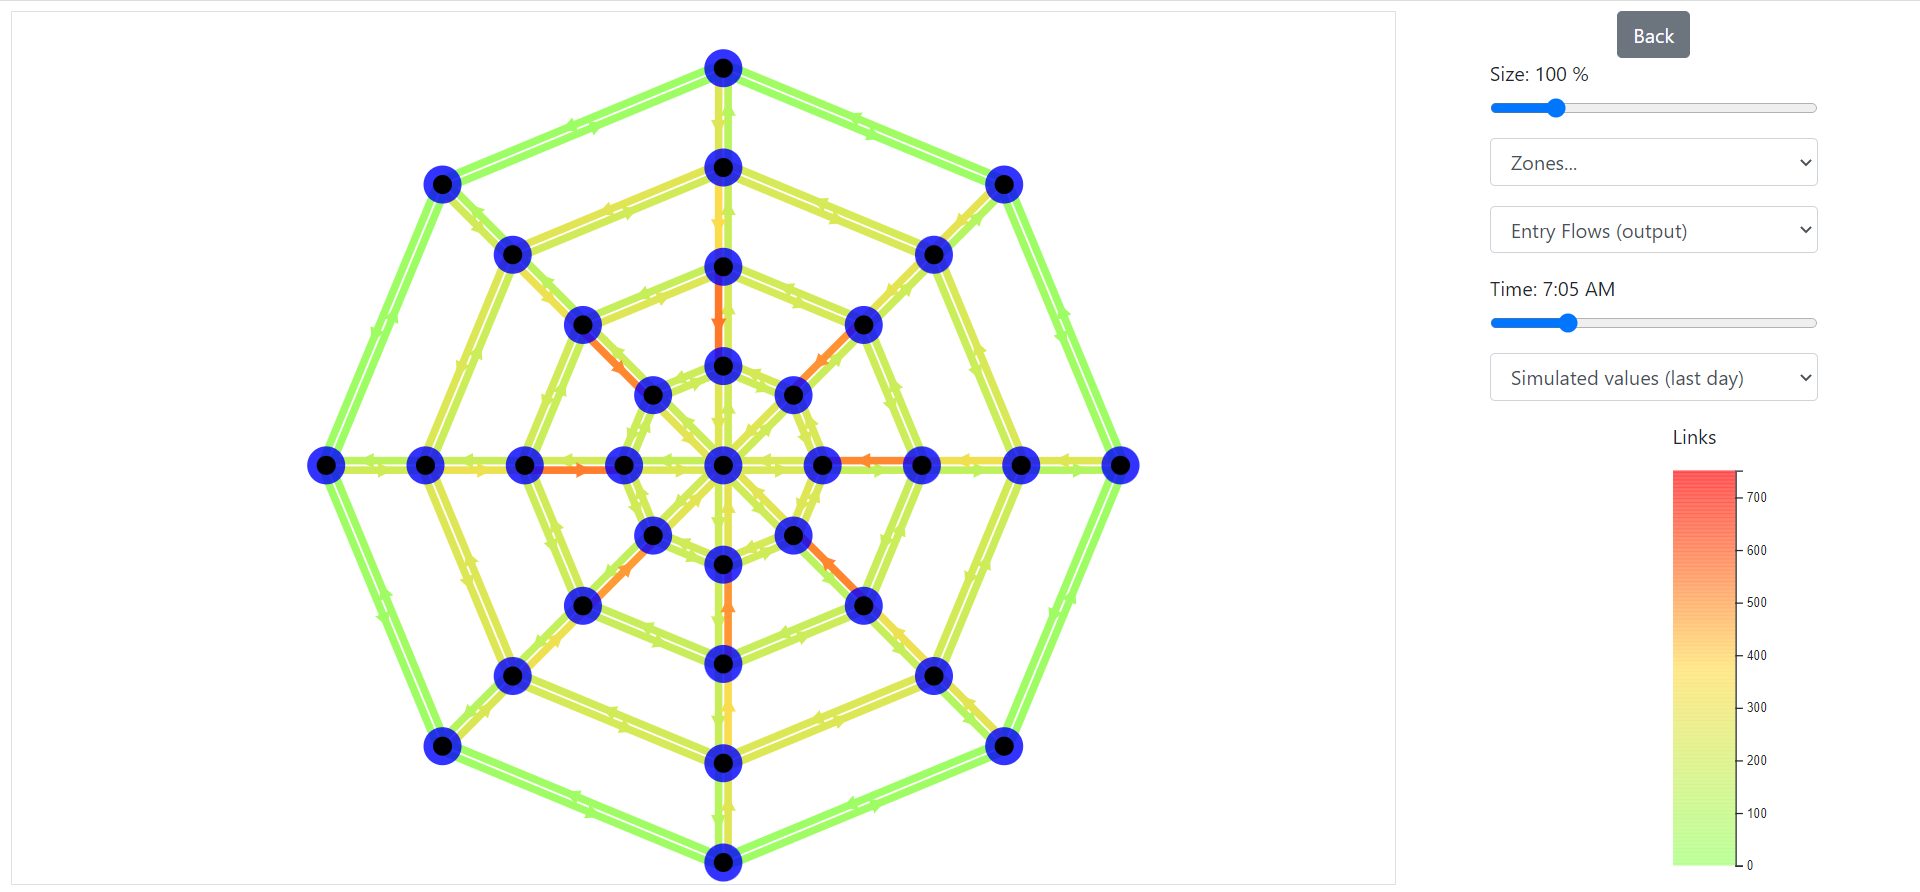
\includegraphics[width=1\textwidth]{Images/Step4/results_on_network__task4.1_705am.png}
    \caption{Entry flows in the network at 7:05 am with constant toll (Task 4.1)}
    \label{fig:Entry flows in the network at 7:05 am with constant toll (Task 4.1)}
\end{figure}
\end{minipage}
\begin{minipage}[c]{0.5\textwidth}
\begin{figure}[H]
    \centering
    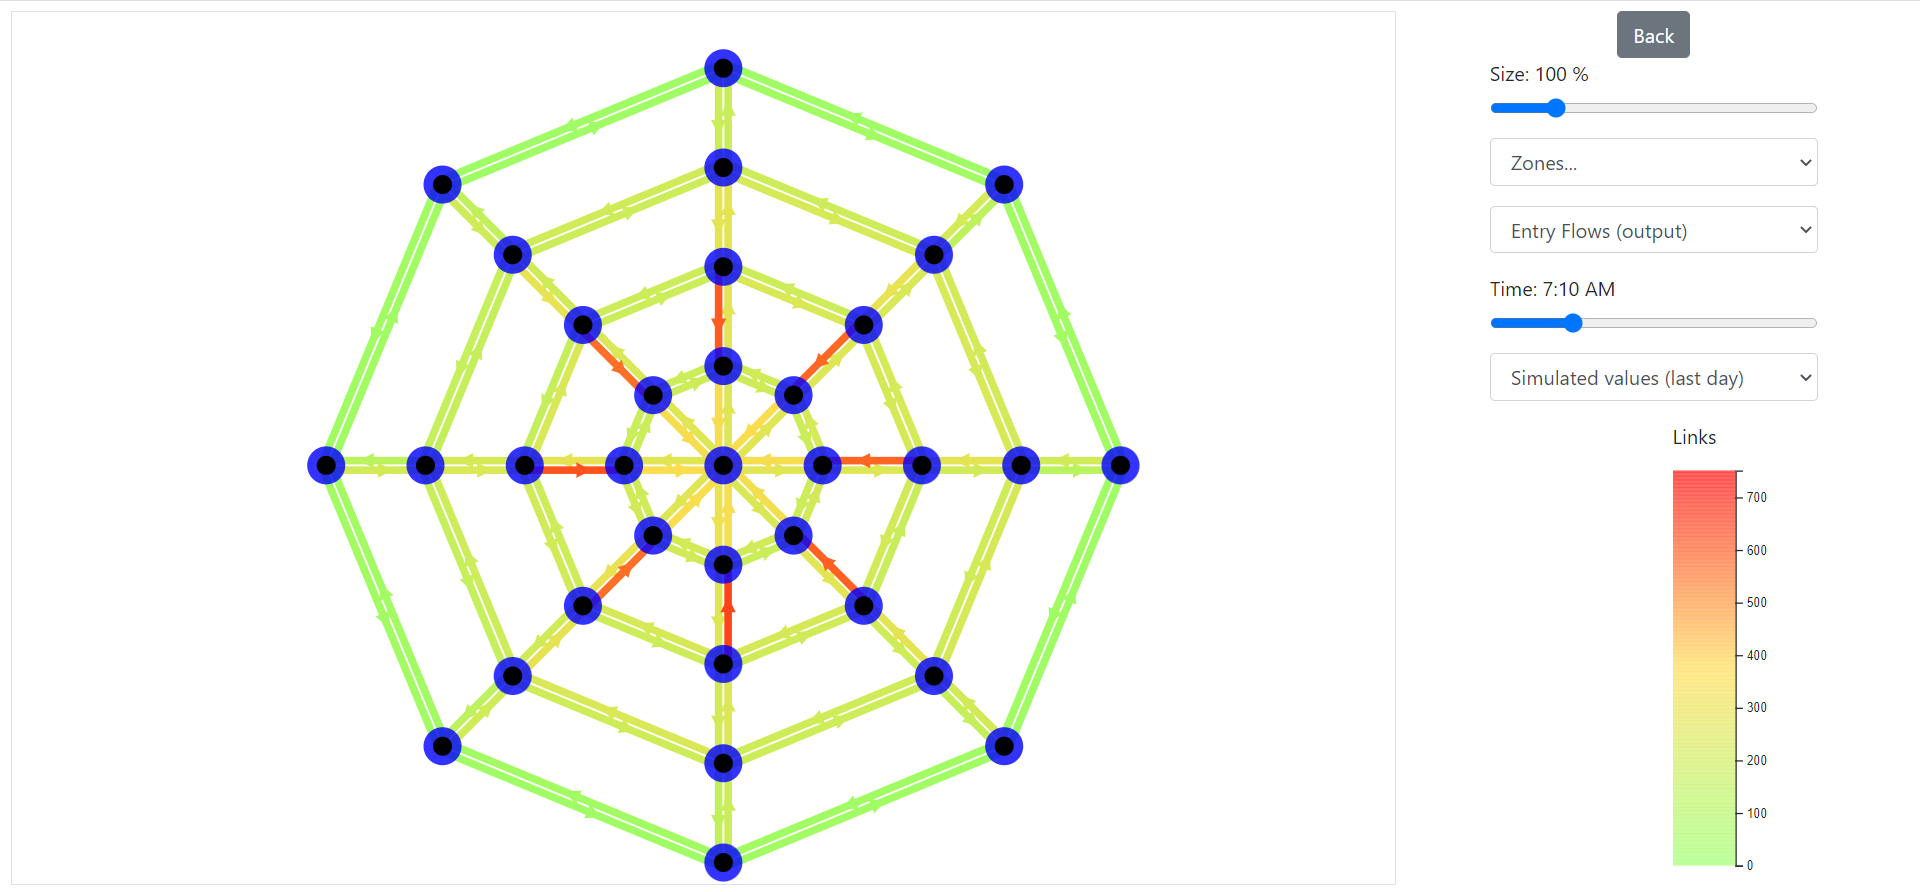
\includegraphics[width=1\textwidth]{Images/Step4/results_on_network__task4.1_710am.png}
    \caption{Entry flows in the network at 7:10 am with constant toll (Task 4.1)}
    \label{fig:Entry flows in the network at 7:10 am with constant toll (Task 4.1)}
\end{figure}
\end{minipage}
\begin{minipage}[c]{0.5\textwidth}
\begin{figure}[H]
    \centering
    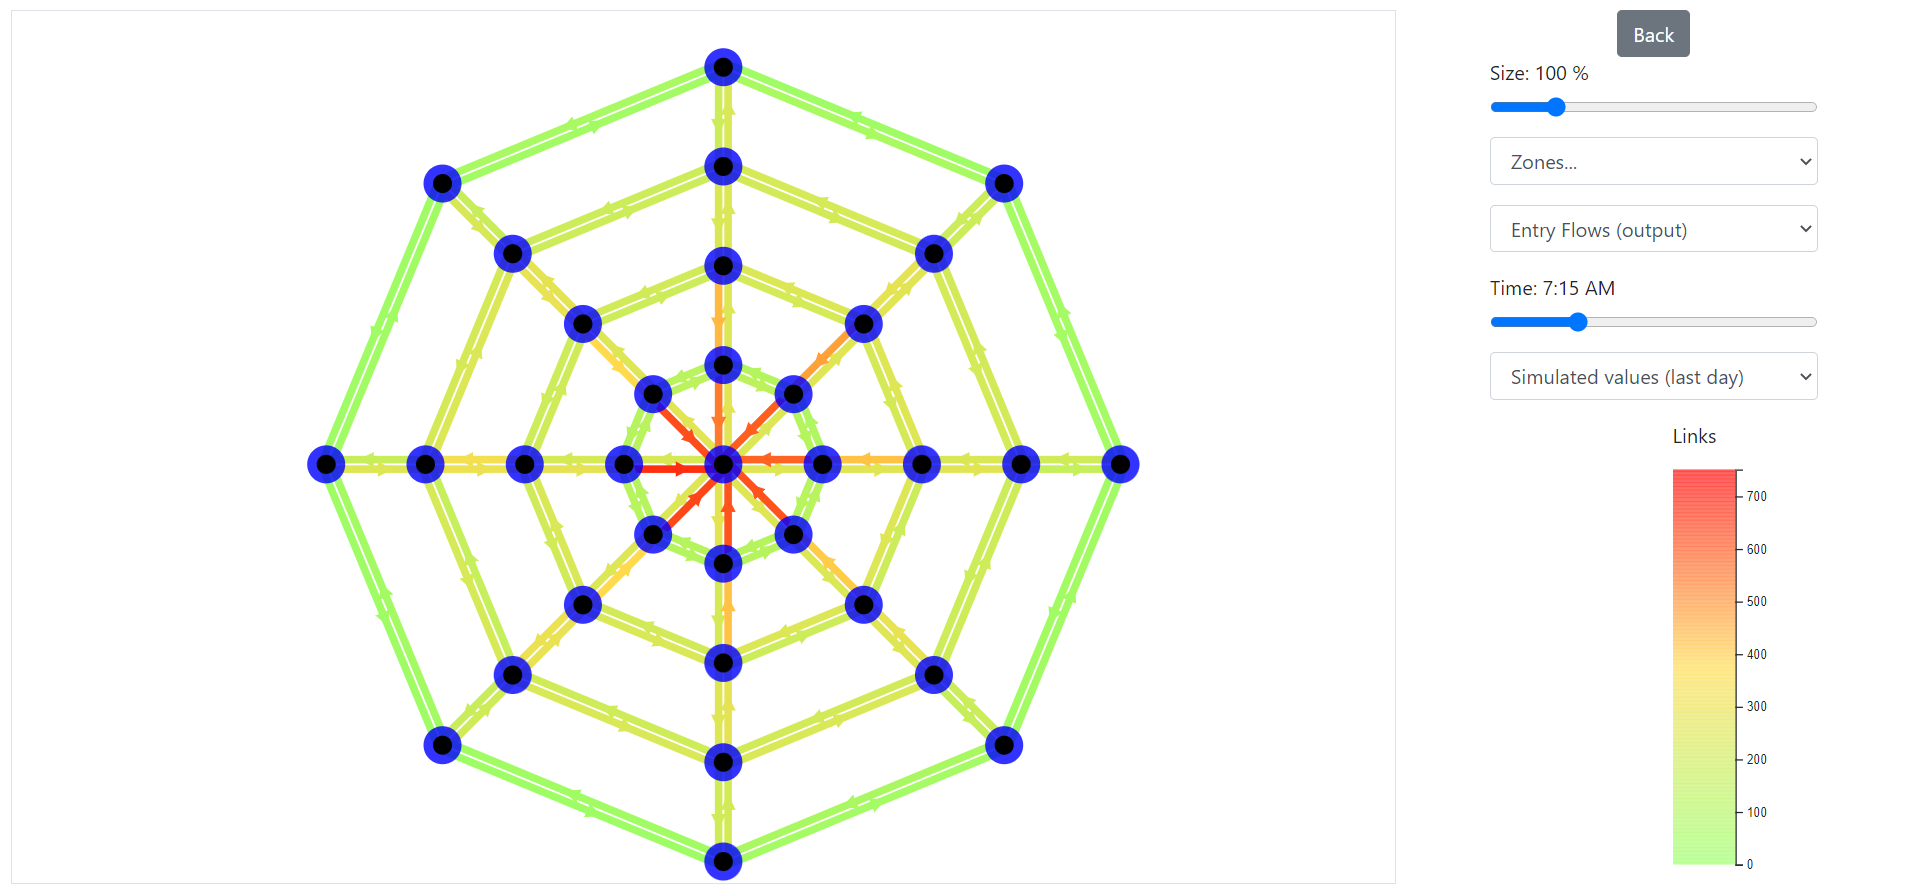
\includegraphics[width=1\textwidth]{Images/Step4/results_on_network__task4.1_715am.png}
    \caption{Entry flows in the network at 7:15 am with constant toll (Task 4.1)}
    \label{fig:Entry flows in the network at 7:15 am with constant toll (Task 4.1)}
\end{figure}
\end{minipage}
\begin{minipage}[c]{0.5\textwidth}
\begin{figure}[H]
    \centering
    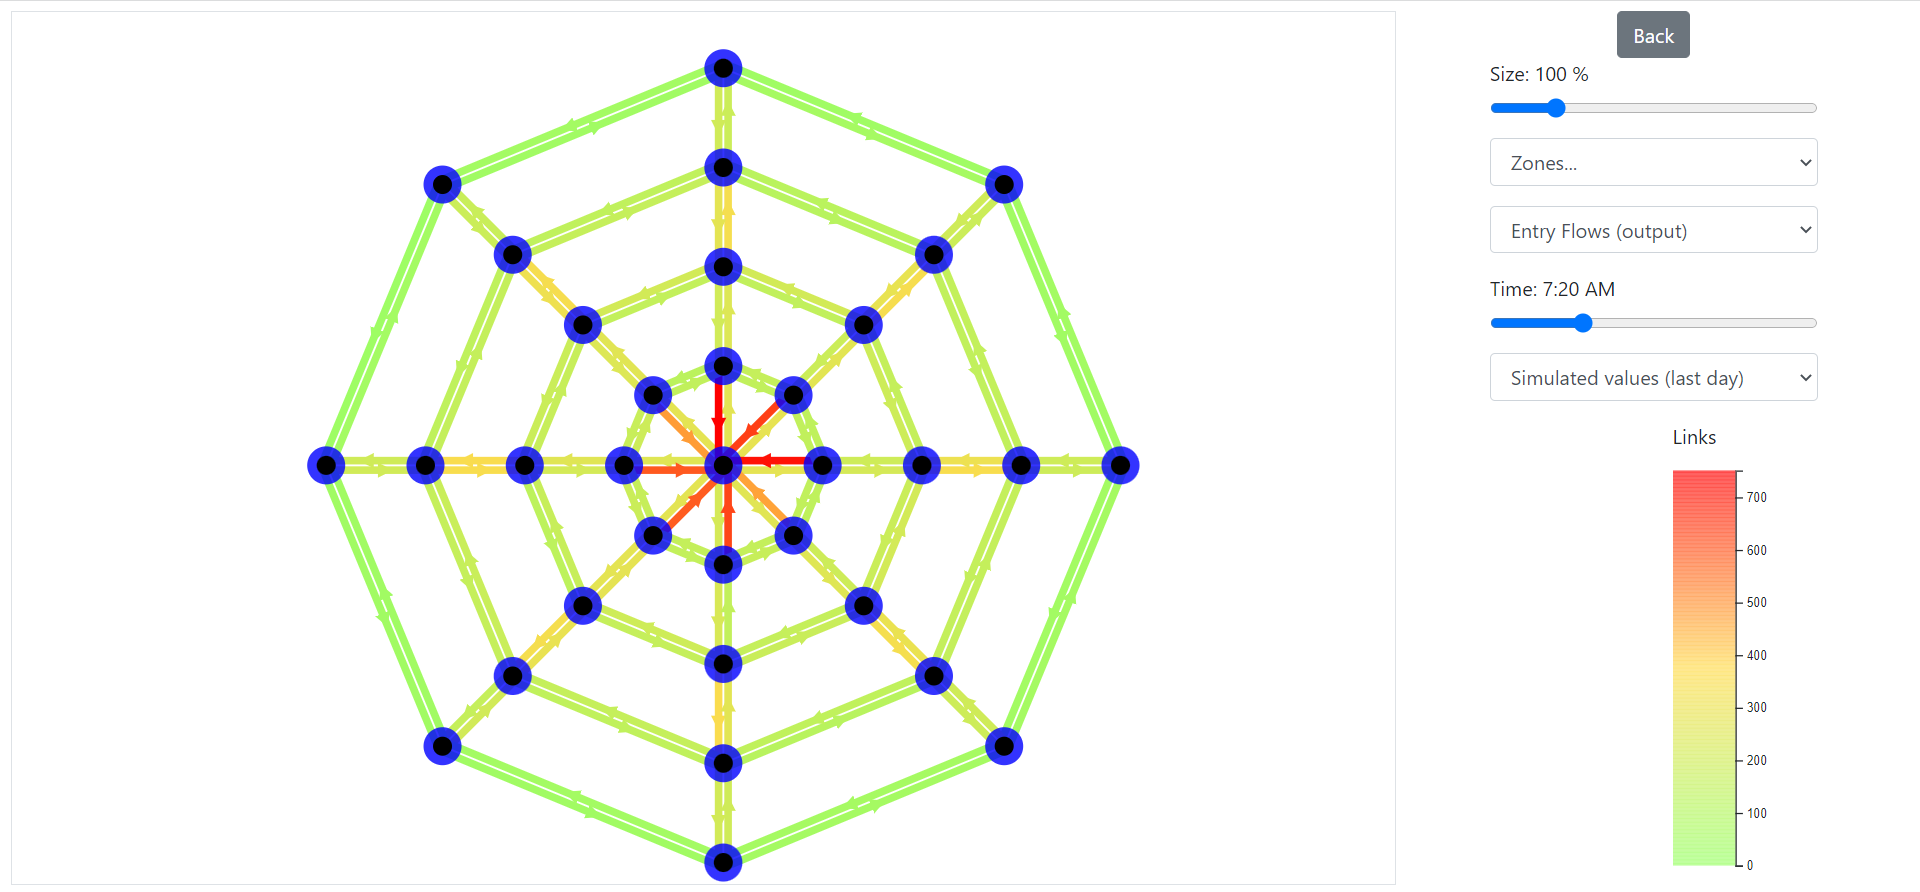
\includegraphics[width=1\textwidth]{Images/Step4/results_on_network__task4.1_720am.png}
    \caption{Entry flows in the network at 7:20 am with constant toll (Task 4.1)}
    \label{fig:Entry flows in the network at 7:20 am with constant toll (Task 4.1)}
\end{figure}
\end{minipage}
\begin{minipage}[c]{0.5\textwidth}
\begin{figure}[H]
    \centering
    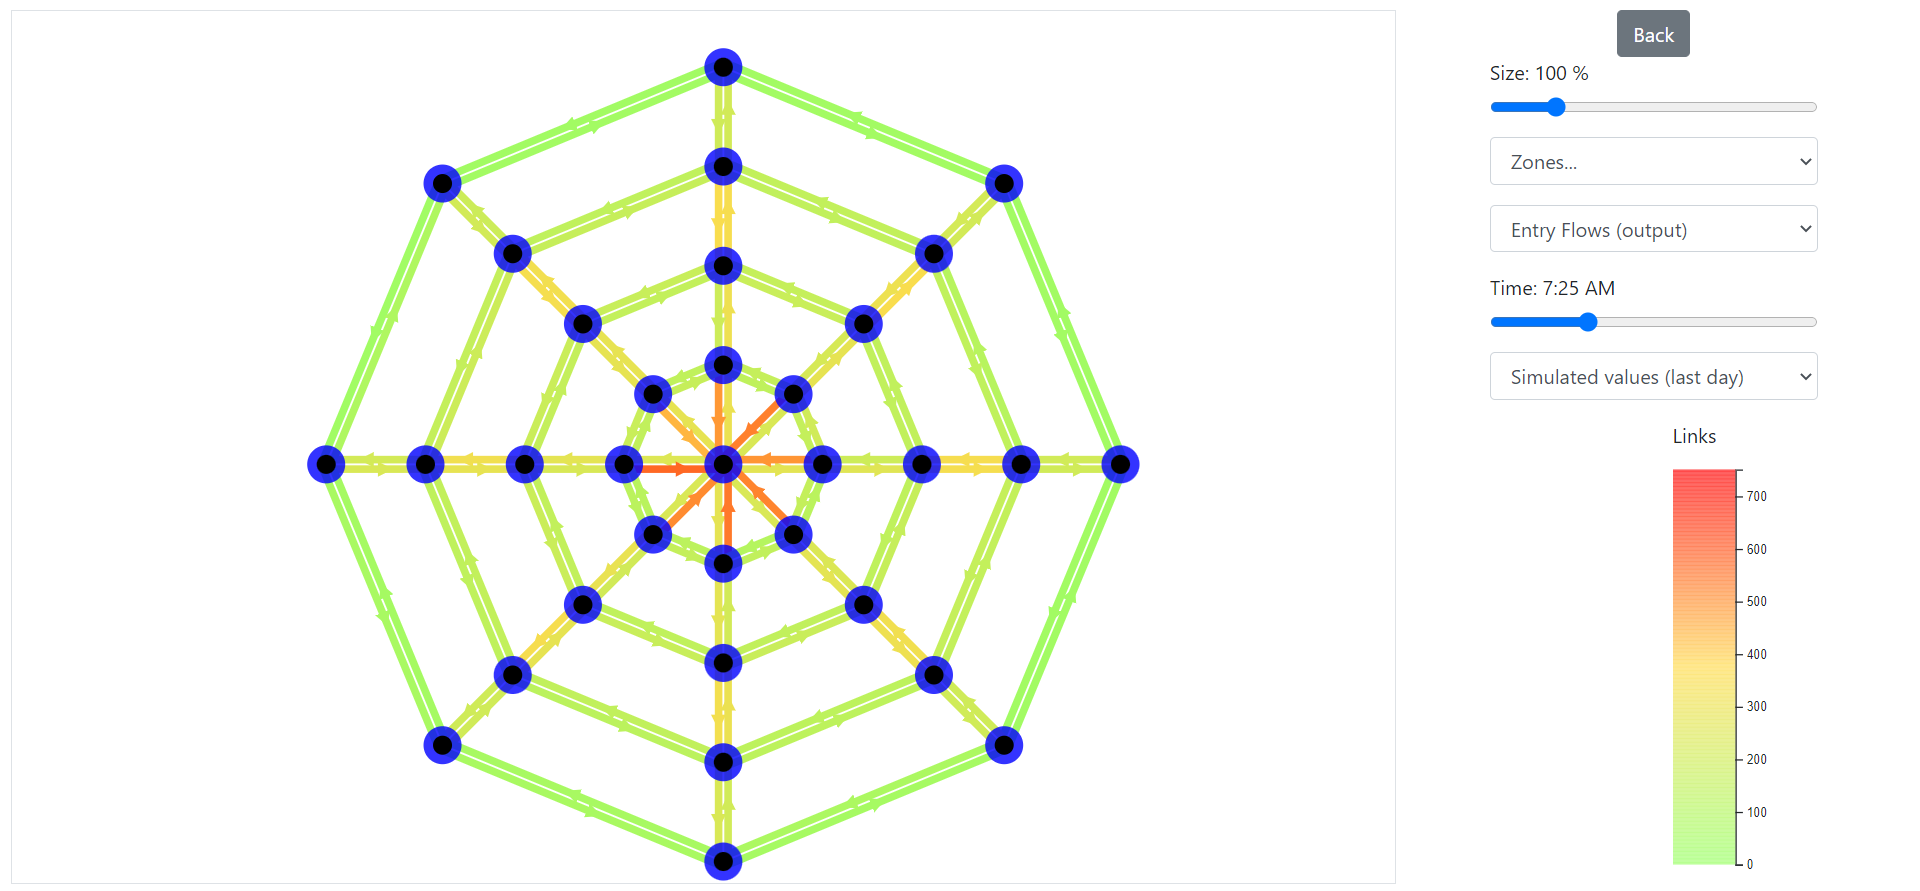
\includegraphics[width=1\textwidth]{Images/Step4/results_on_network__task4.1_725am.png}
    \caption{Entry flows in the network at 7:25 am with constant toll (Task 4.1)}
    \label{fig:Entry flows in the network at 7:25 am with constant toll (Task 4.1)}
\end{figure}
\end{minipage}
\begin{minipage}[c]{0.5\textwidth}
\begin{figure}[H]
    \centering
    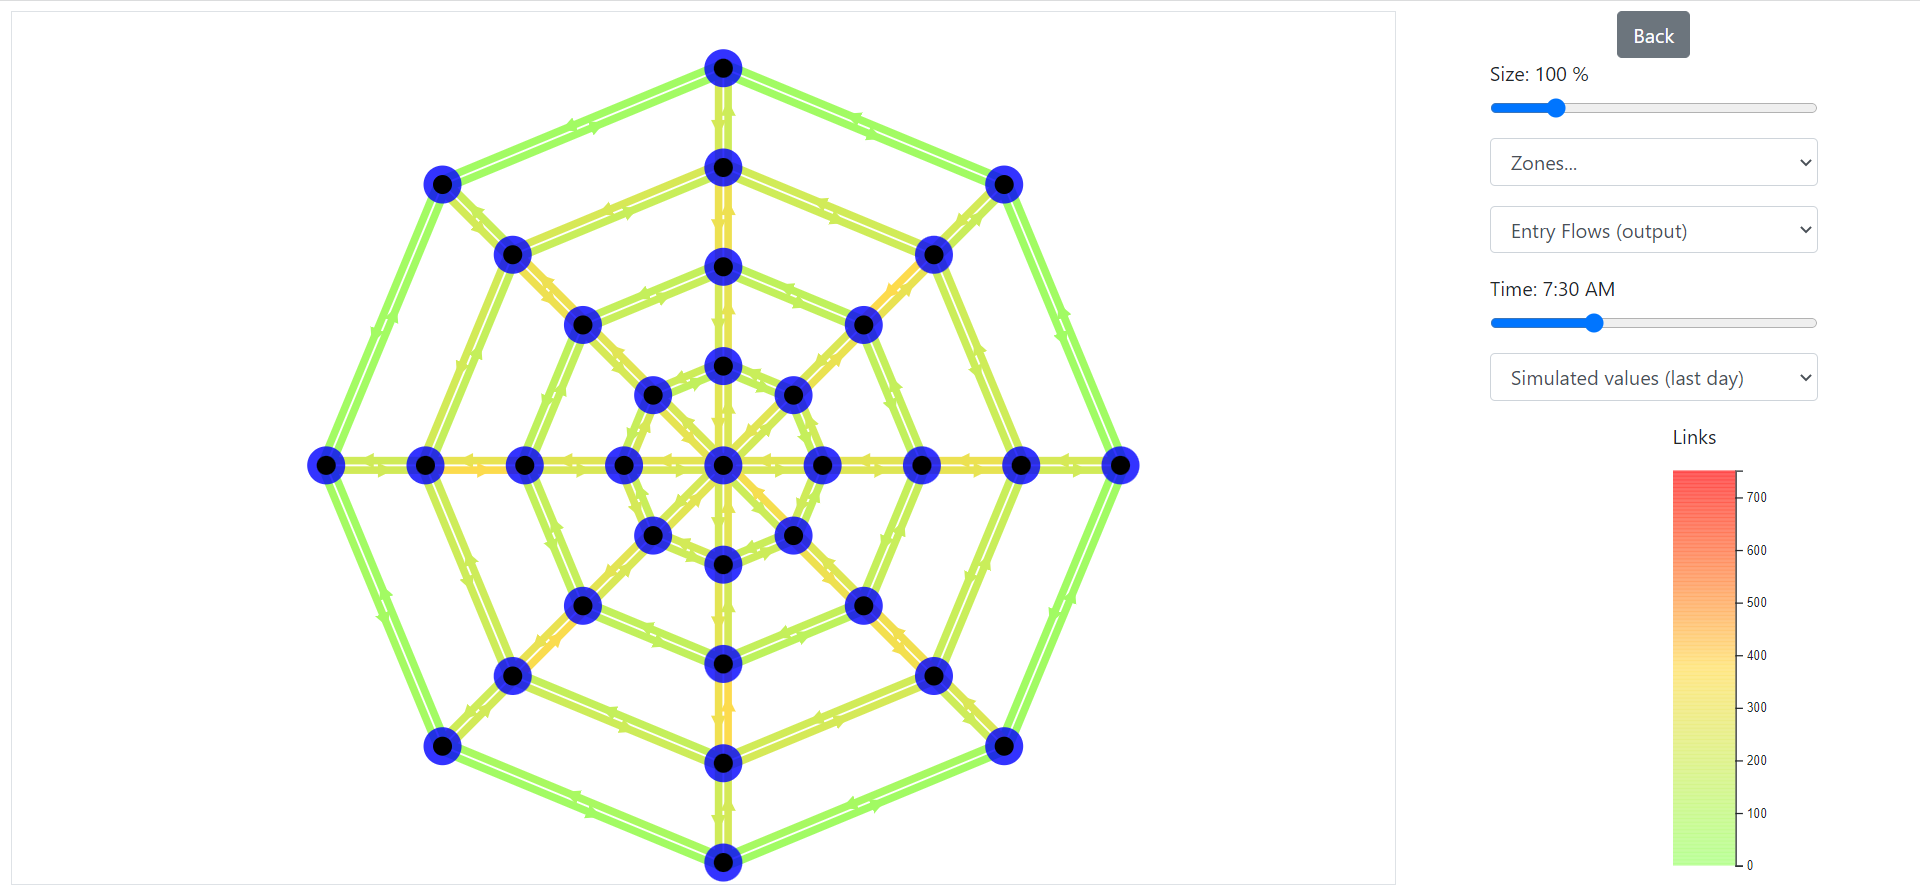
\includegraphics[width=1\textwidth]{Images/Step4/results_on_network__task4.1_730am.png}
    \caption{Entry flows in the network at 7:30 am with constant toll (Task 4.1)}
    \label{fig:Entry flows in the network at 7:30 am with constant toll (Task 4.1)}
\end{figure}
\end{minipage}
\\

These observations allow us to draw several conclusions.\\

The first is that the intensity of the flows observed is caused by the fact that a large proportion of users want to go to the city centre at the same time. This causes heavy congestion. It is interesting to ask why there is such a concentration. The answer seems obvious. These large flows occur from 7:15 am onwards, the time at which the toll is lifted. As a result, people enter the city centre en masse after this time to avoid paying the toll. This behaviour causes severe congestion on the network. This also explains why the city centre was practically empty before this time.\\

The second conclusion we can draw is related. Through all these representations, we notice that the flows occur later in the morning than in Task 2. This is logical. Not wanting to pay the toll, users will arrive later in the city centre and leave home later. There was no such issue in the Task 2 configuration, so there is an impact of this pricing policy on the users' choice of departure time.\\

Although this second conclusion seems to be the most logical, there could be another phenomenon that could act in parallel to the delayed departures and explain, in part, this delayed entry to the city centre. It could be that some people leave home at the same time as in Task 2 but instead of entering downtown directly (as before), they wait at the edge of the inner ring to enter only at the end of the fare period. This possibility could happen in reality. However, it does not appear to us to explain the results observed here. People engaging in this behaviour would lose time at the downtown curb. There is no benefit to them. The advantage they might gain is that they would be in the first position to leave once the toll is lifted. This would allow them to get to work on time without having to pay the toll. So they would have an advantage in doing that.\\

From what we have been able to discuss, this model does not cover this option and this phenomenon should not occur in this case, but again, it is quite possible that such a phenomenon could occur in reality.\\



\subsubsection{Effect of the toll on congestion, customer surplus and number of public transport users}
It is interesting to study the effects of such a road pricing policy on congestion, consumer surplus and the number of users using public transport (instead of the car). To do so, we generated a graph for each of these three variables as a function of iterations. This allows us to comment on the situation at the end of the iterations, but also on the evolution of the studied characteristics.\\

In addition, in order to be able to study other influences, we have also provided graphs for speed and travel time as well as for the ratios (early, on time and late).\\

Firstly, we are interested in the effects of this pricing on congestion. First, we observe that the toll strategy is more attractive than the no-toll strategy. Congestion falls drastically during the first iterations and continues to fall more slowly afterwards. This can be explained by the fact that during the very first days of the simulations, all users will act naively and find themselves in the middle of the peak full stop in traffic jams. But this time, in addition, they will have to pay a toll. As a result, many of them will certainly change their departure time or switch to public transport to avoid this situation.\\

\begin{figure}[H]
    \centering
    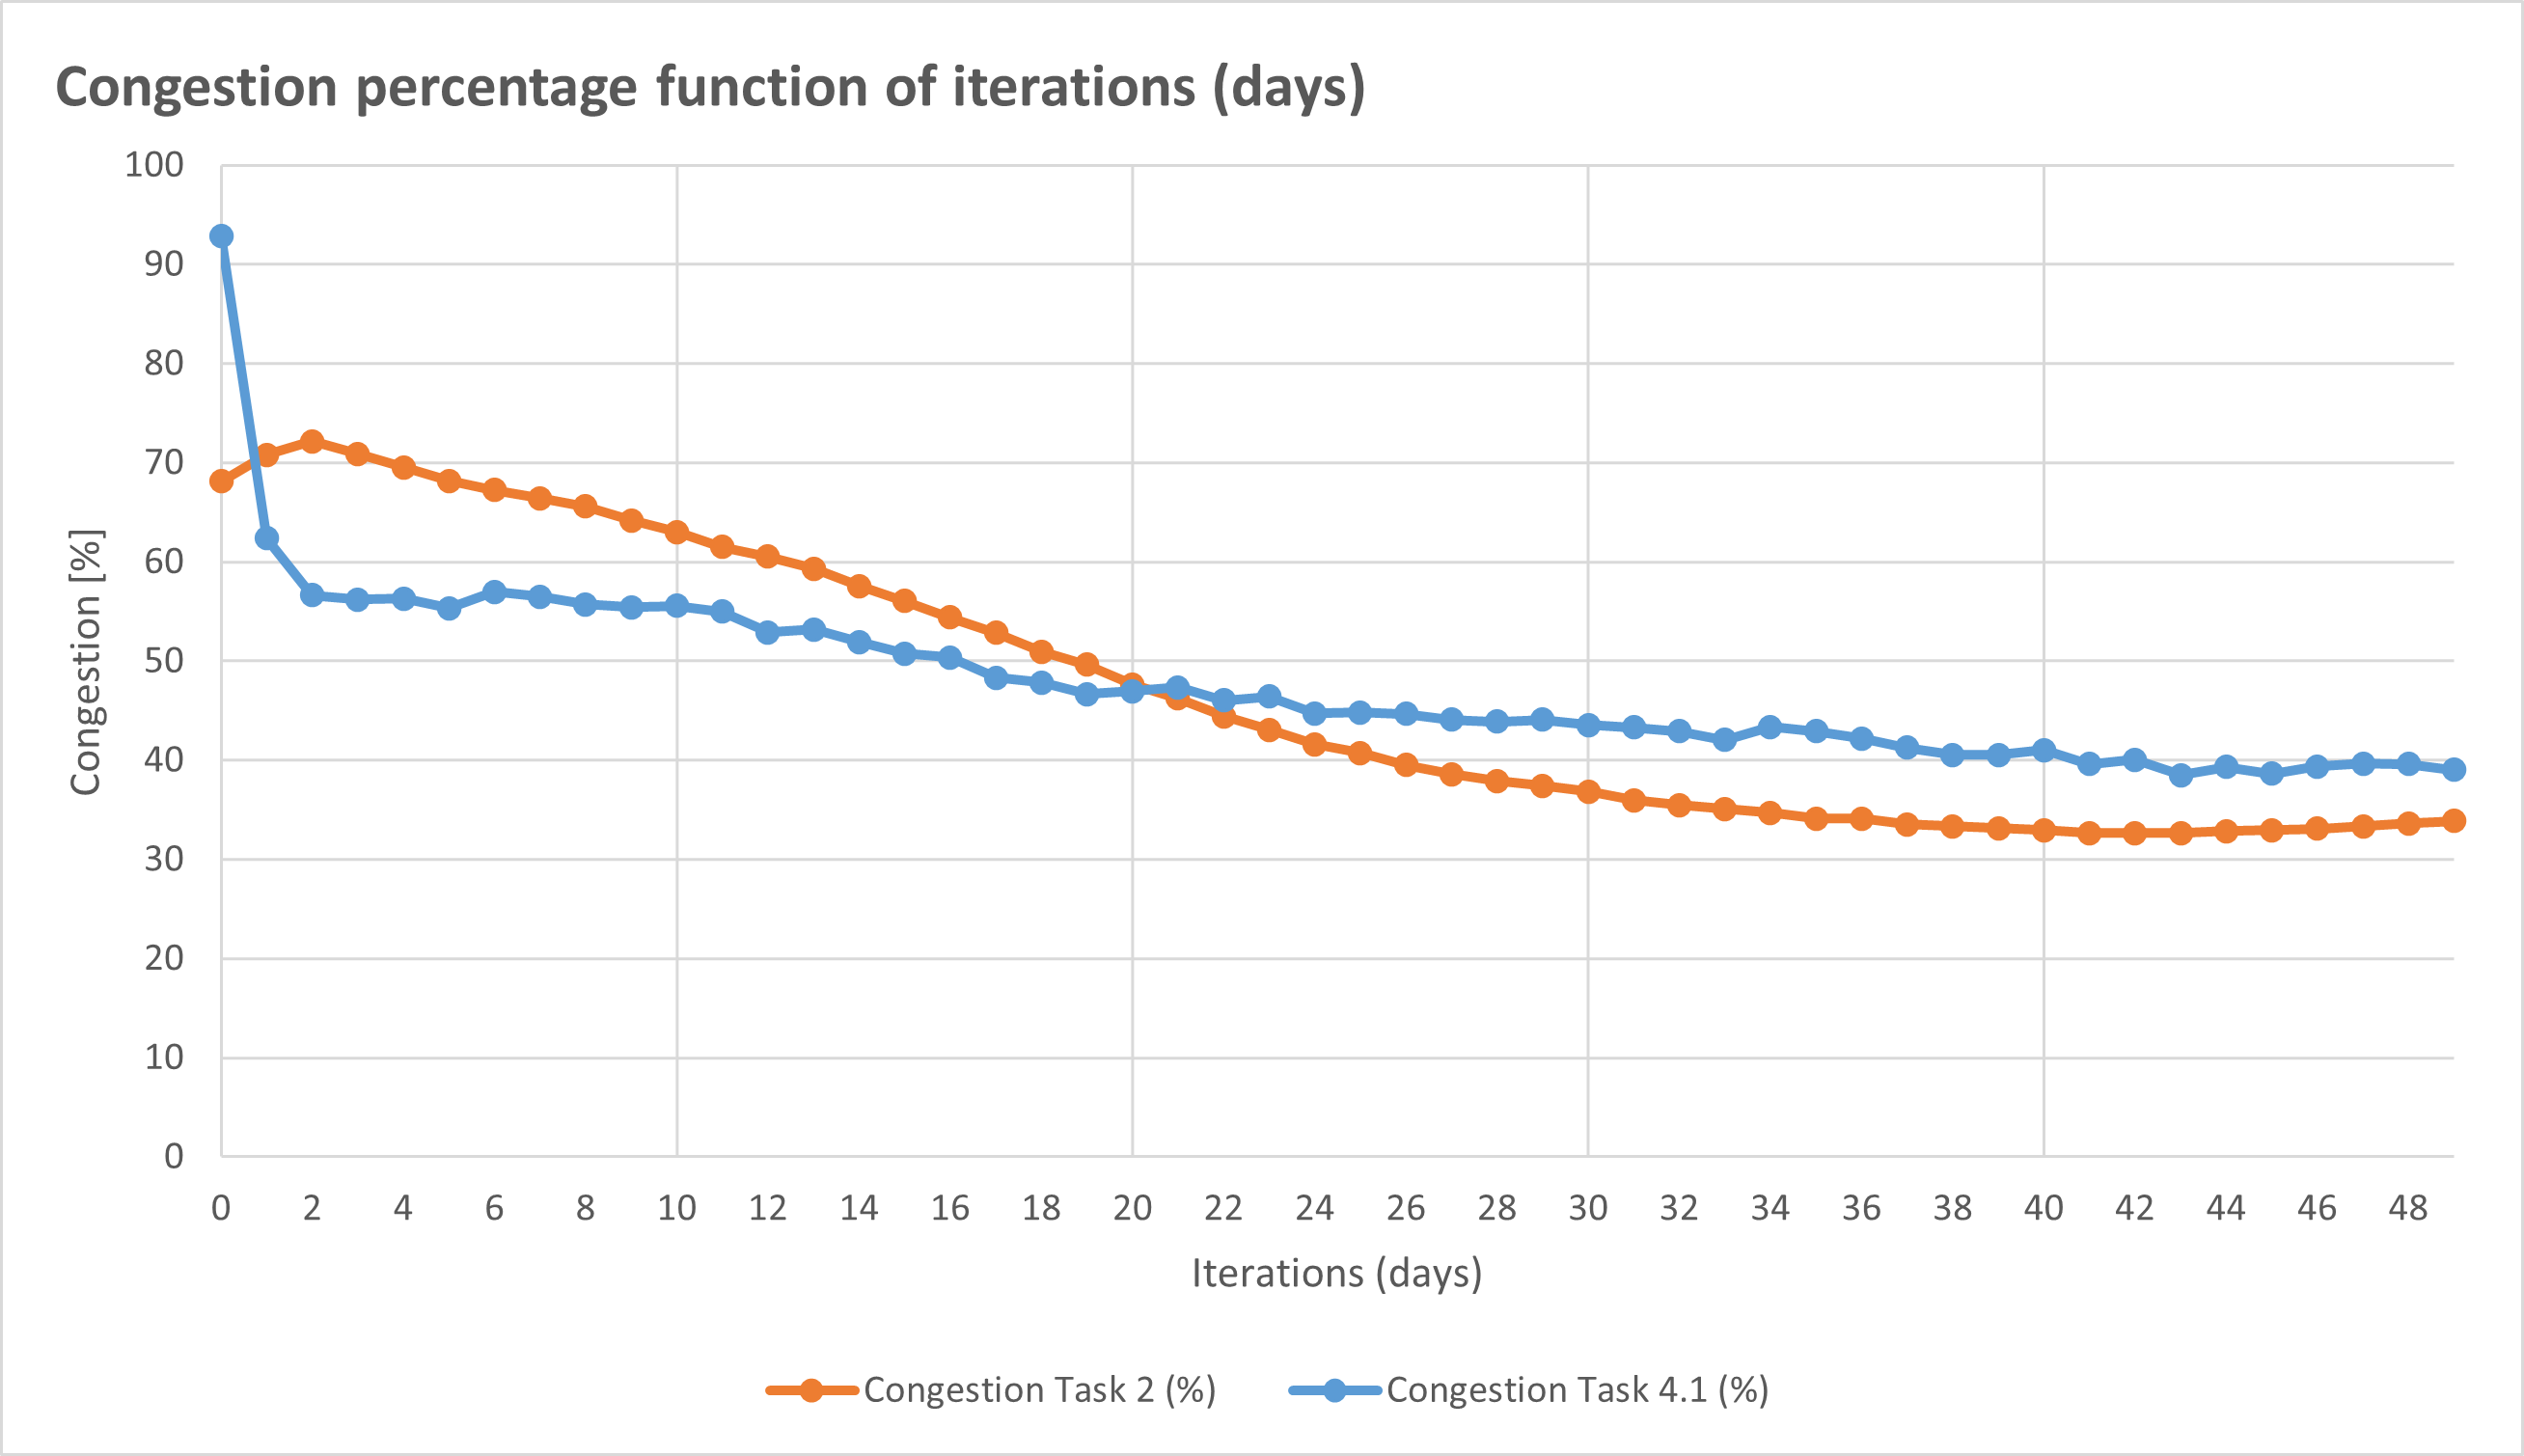
\includegraphics[width=0.8\textwidth]{Images/Step4/Congestion_percentage_function_iterations_comparaison_task_2_4.1.png}
    \caption{Congestion percentage function of iterations for the task 2 and 4.1 (days)}
    \label{fig:Congestion percentage function of iterations for the task 2 and 4.1 (days)}
\end{figure}

However, around the twentieth iteration, as the curve of Task 4.1 decreases less strongly than that of Task 2, the two curves cross and the congestion rate in the new configuration is higher than in the situation without pricing. This trend continues until the end of the iterations and the congestion rate in the priced situation is thus higher (+5.14\%) than in the previous state. This difference in decrease can perhaps be explained by the way the pricing is applied. Recall that the toll must be paid for anyone entering the city centre before 7:15 am. As we have said, initially, because of the very high congestion and the need to pay the toll, a large number of people will change their behaviour, most likely by changing their mode of transport. This will leave drivers who do not wish to change their mode of transport. Their only other real alternative is to leave home earlier. However, as they have to pay the toll before 7:15 am, they will pay it in any case (whether they arrive in the city centre at a time of heavy congestion or earlier). Therefore, they are likely to say to themselves that they don't want to pay and also arrive much too early. The advance is therefore less acceptable than in the first situation. This may explain why congestion decreases but is less than in the case without charge. This results in a situation with more congestion than without tolling. The situation is therefore less favourable.\\

Another behaviour that can explain this high level of congestion is the one provided in the previous section.\\

Drivers do not want to pay and be in traffic. Therefore, they will leave home later and arrive at the city centre after the end of the tariff period. They therefore prefer to be in traffic than to have to pay a toll, which reduces the number of people leaving home early.\\

Secondly, we can analyse the effects on consumer surplus. We see directly that the surplus is less favourable in the tariffed situation than in the basic situation. We see that the trend remains comparable (although the new curve is more variable).\\

\begin{figure}[H]
    \centering
    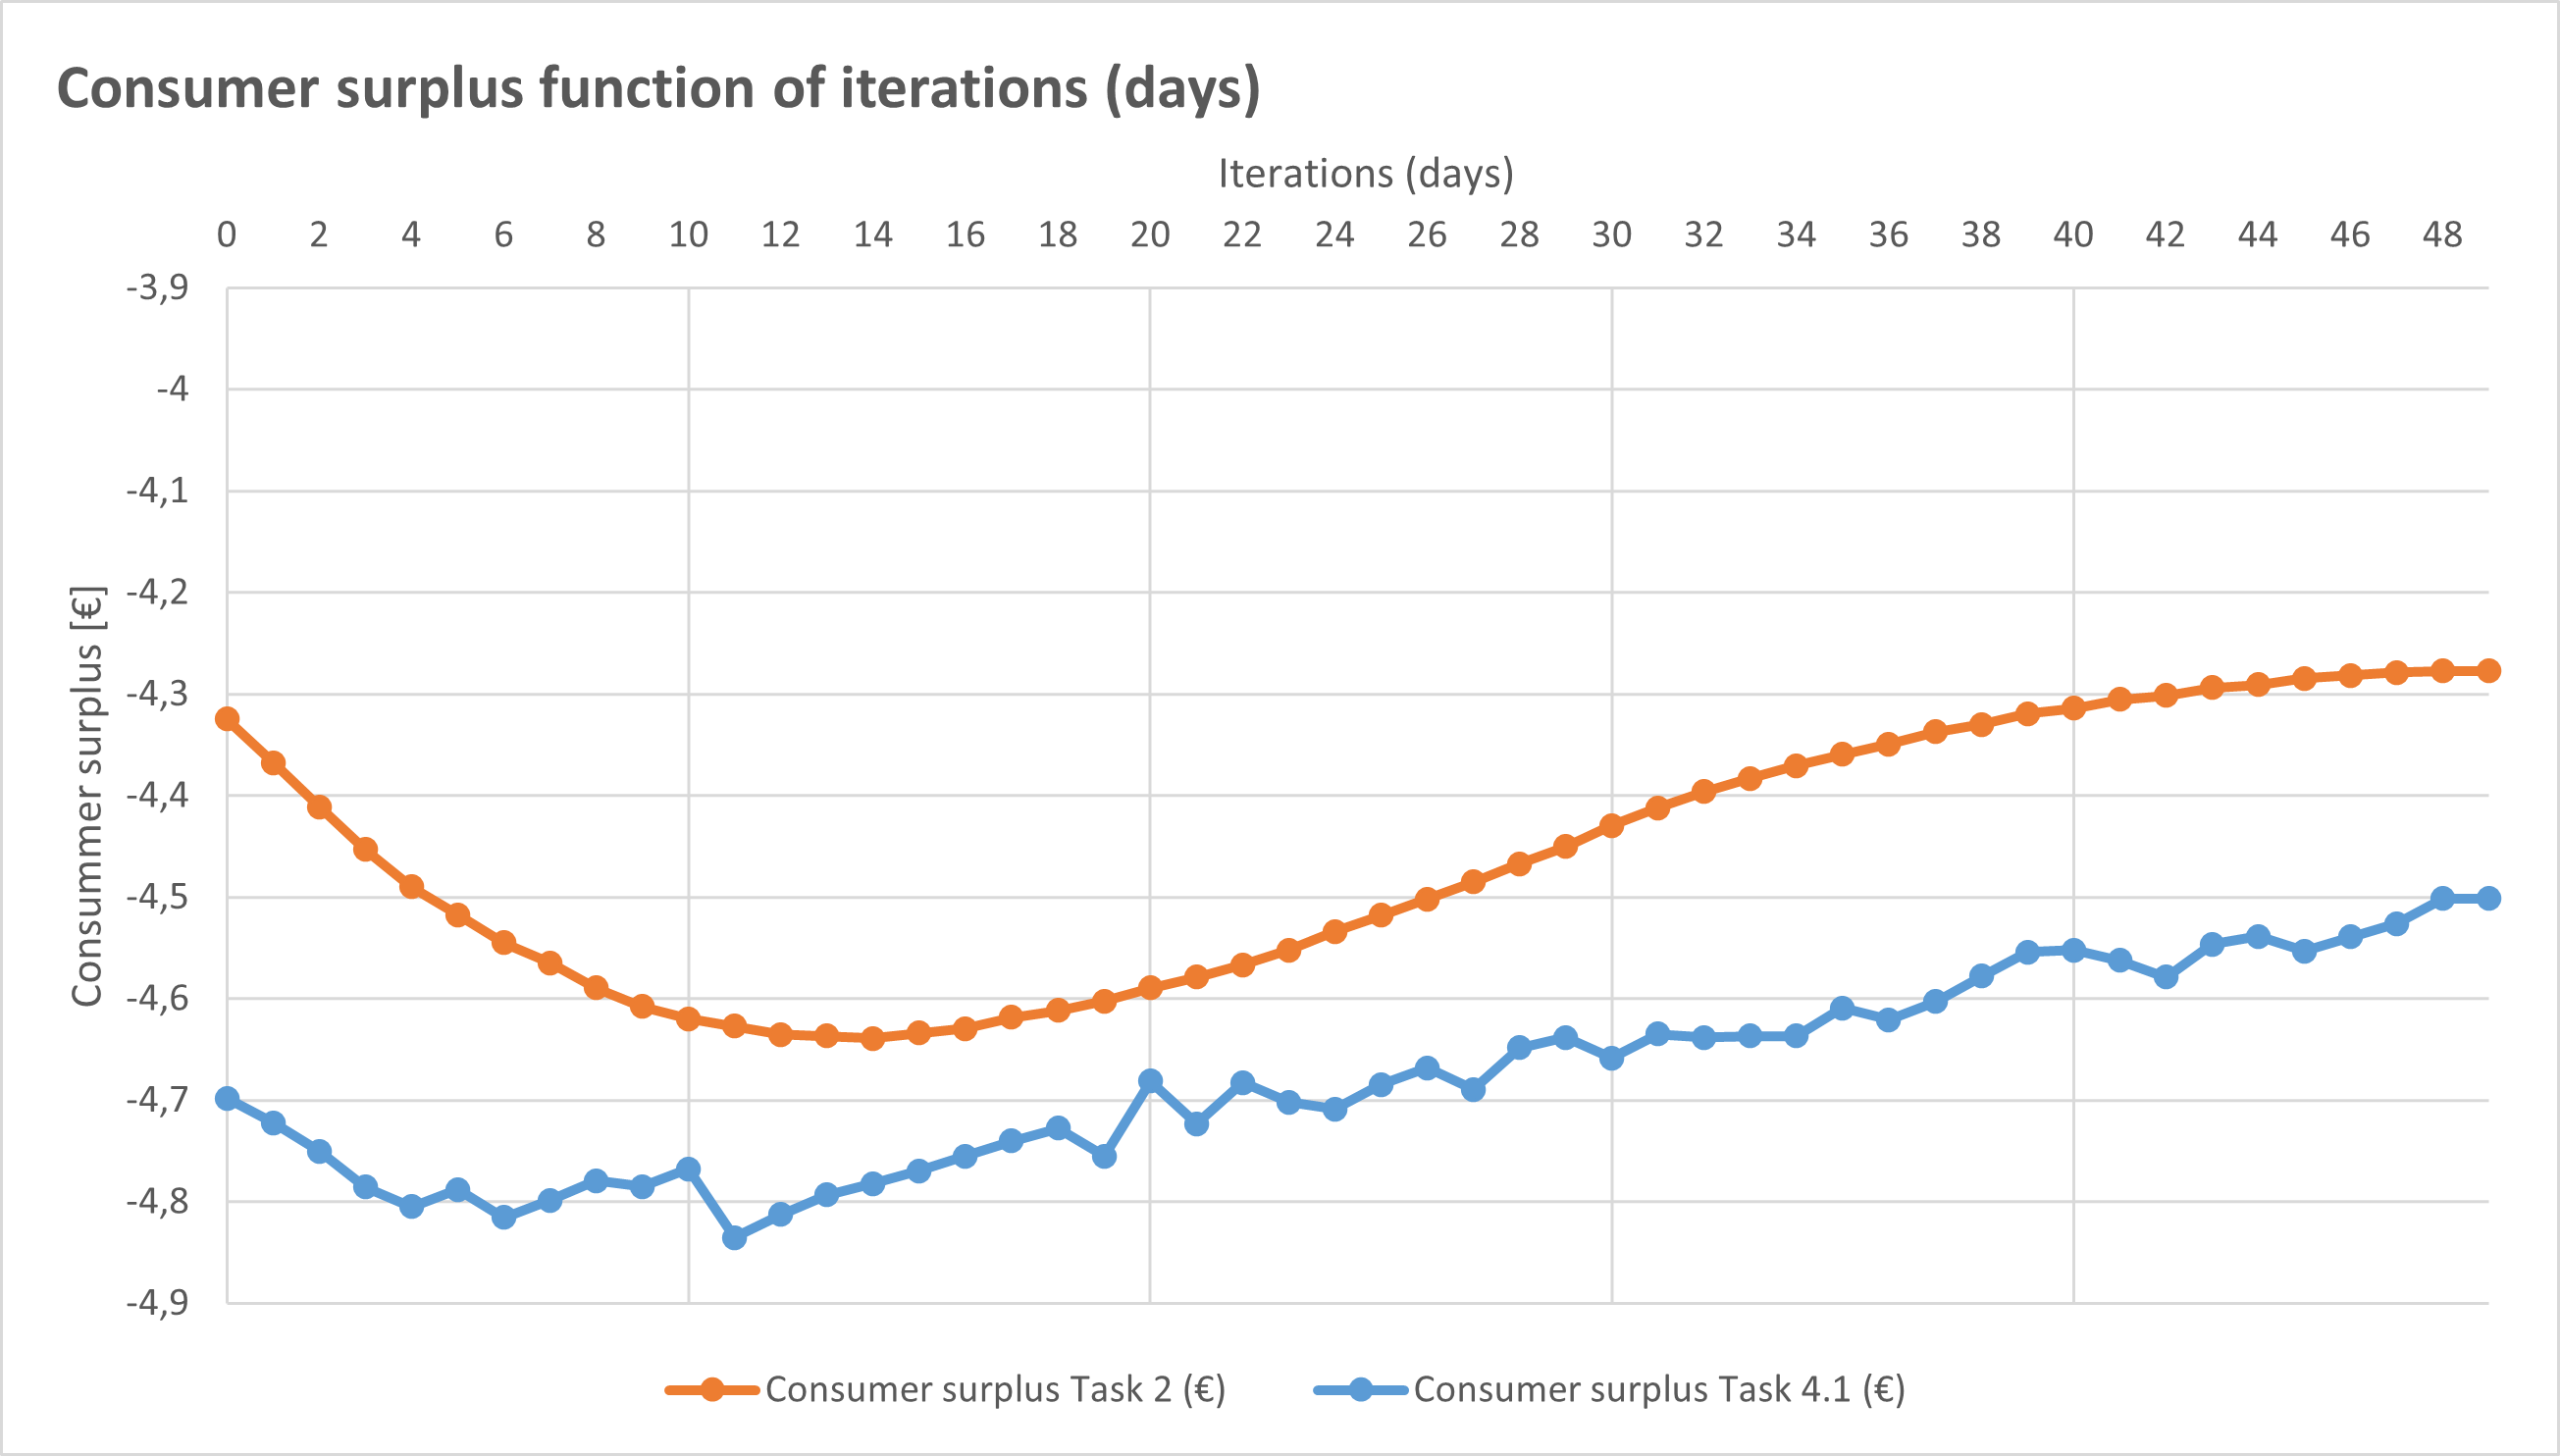
\includegraphics[width=0.8\textwidth]{Images/Step4/Consumer_surplus_function_iterations_comparaison_task_2_4.1.png}
    \caption{Consumer surplus function of iterations for task 2 and 4.1 (days)}
    \label{fig:Consumer surplus function of iterations for the task 2 and 4.1 (days)}
\end{figure}

After an initial period where the new surplus remains relatively stable, it improves from the 10th iteration to the end. This may be the consequence of some of the drivers leaving earlier.\\

At the last iteration, the surplus is lower (-0.22391 [€]) in the paying case. So we see that the situation is less profitable for the users while not being interesting from the congestion point of view.\\


Third, we can study the change in the number of drivers, and consequently in the number of public transport users, as a function of the iterations.\\


\begin{figure}[H]
    \centering
    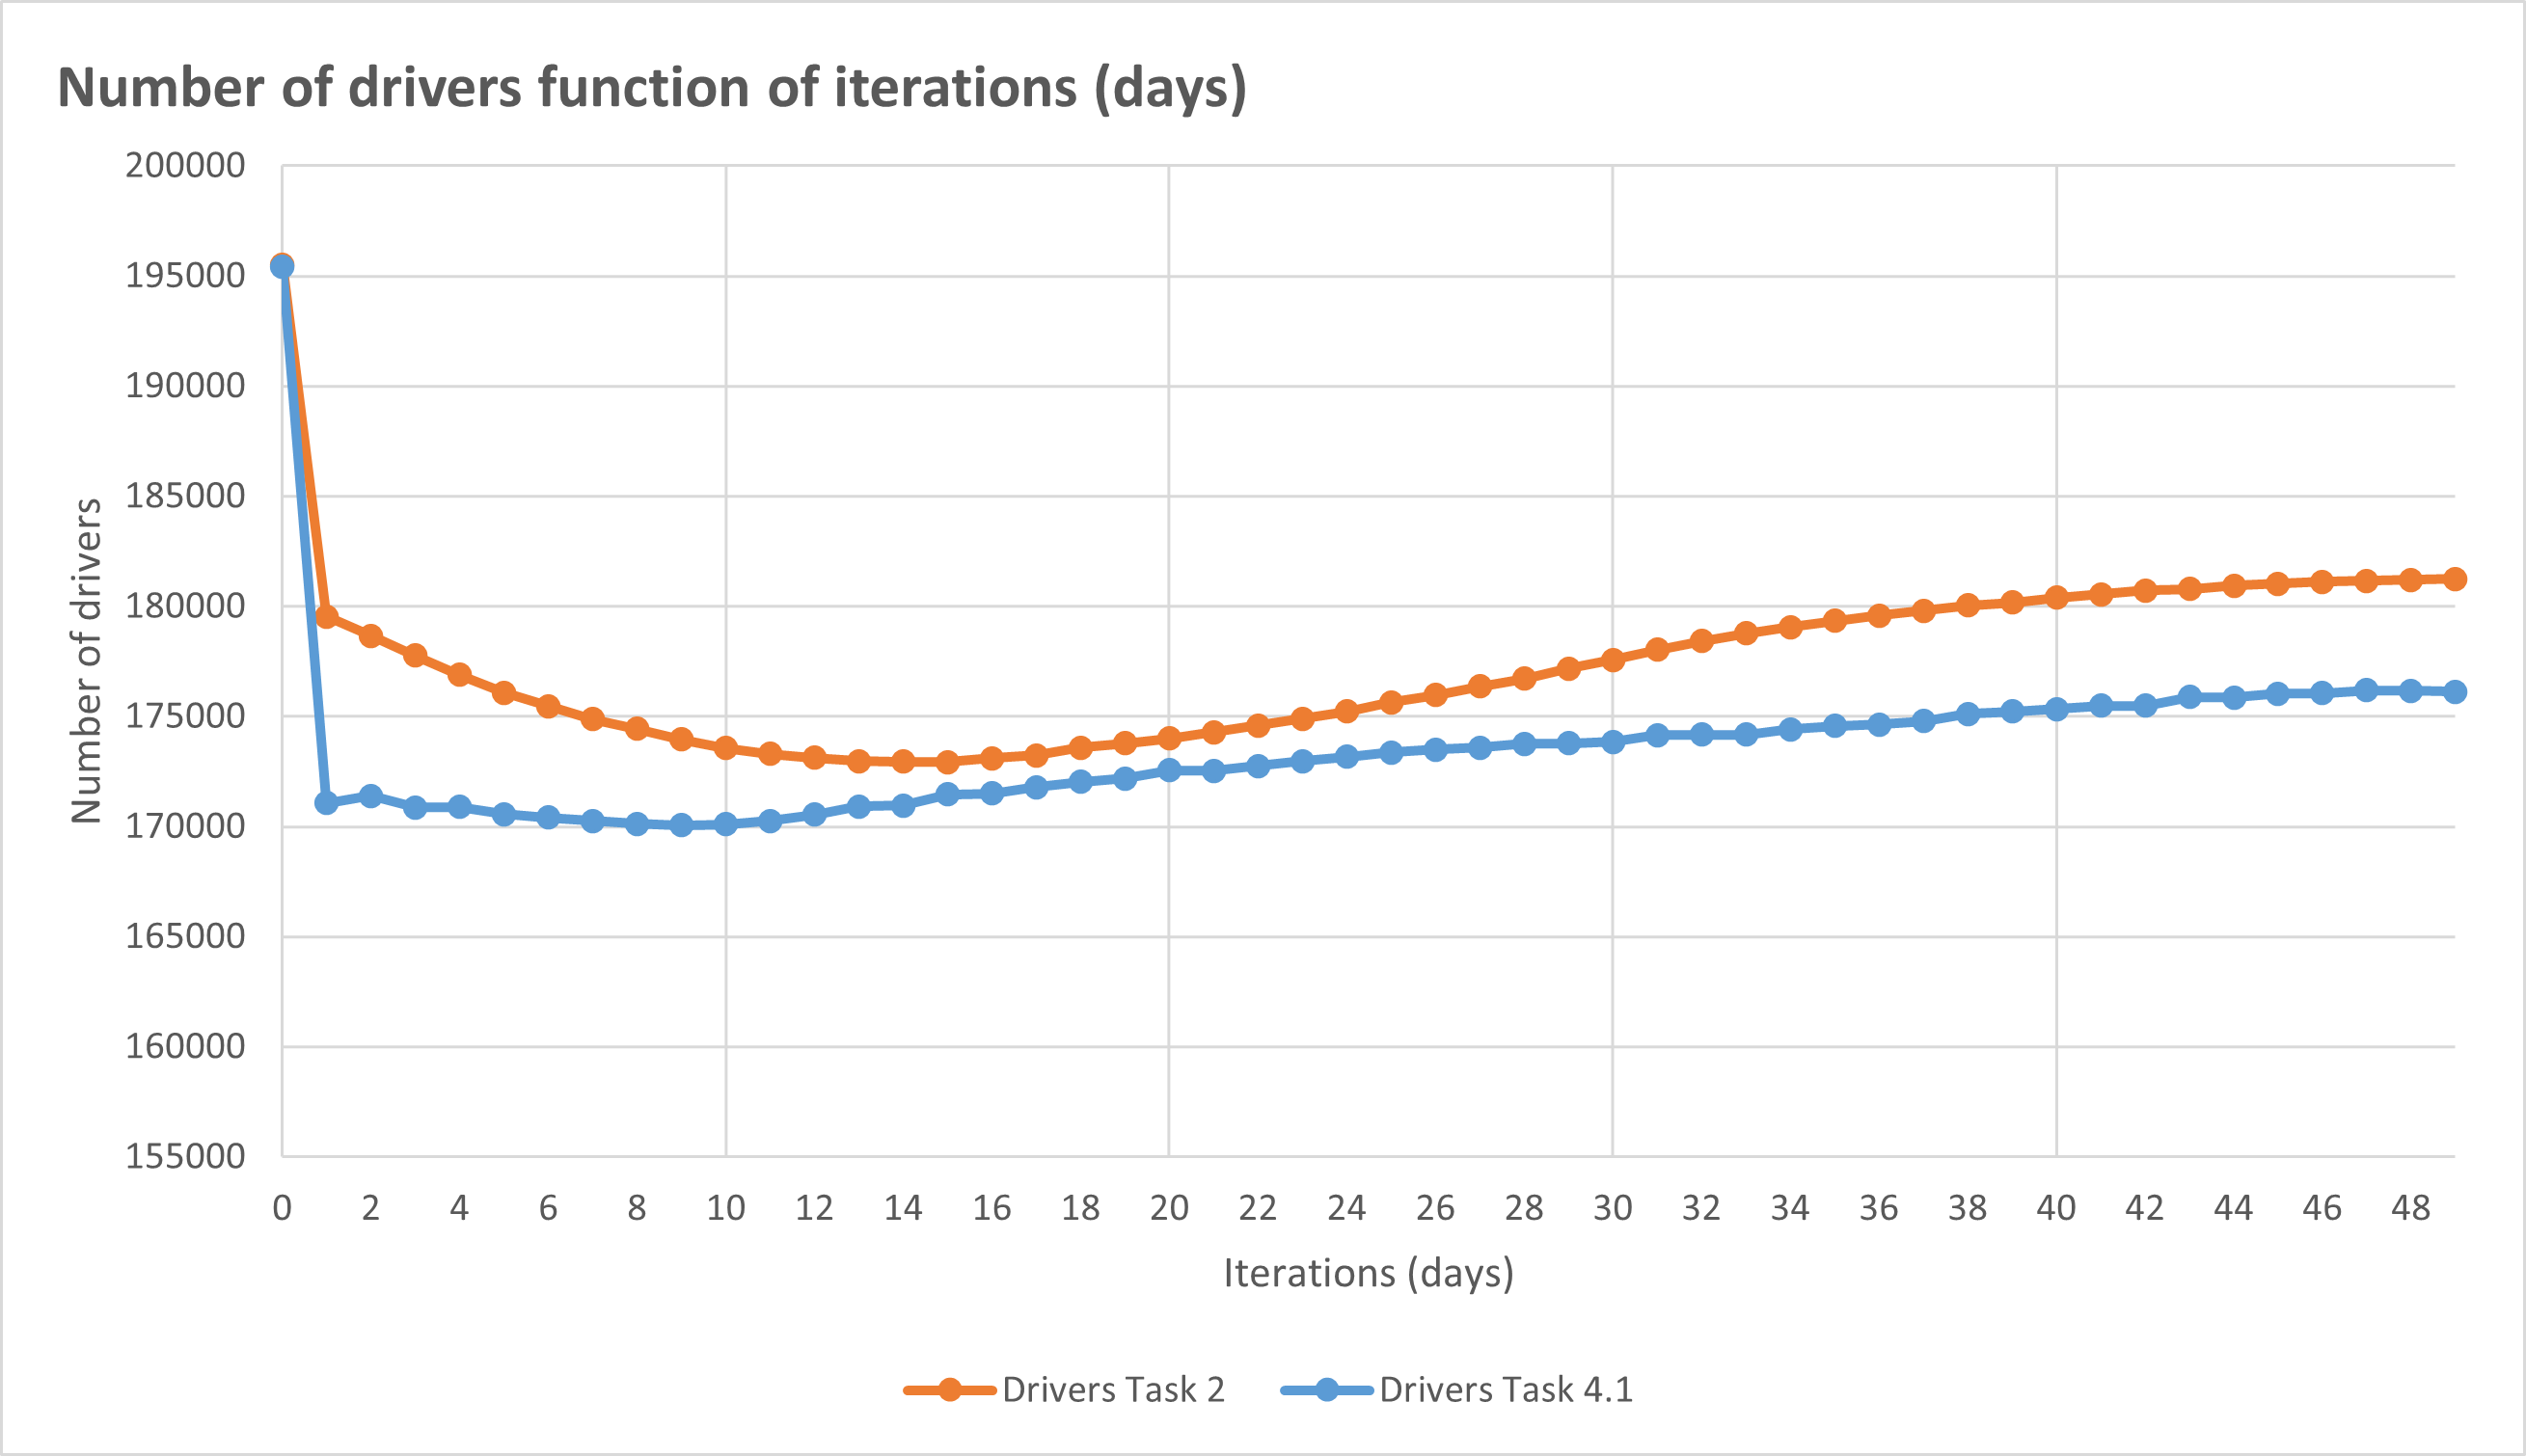
\includegraphics[width=0.8\textwidth]{Images/Step4/number_drivers_function_iterations_comparaison_task_2_4.1.png}
    \caption{Number of drivers function of iterations for the task 2 and 4.1 (days)}
    \label{fig:Number of drivers function of iterations for the task 2 and 4.1 (days)}
\end{figure}

\begin{figure}[H]
    \centering
    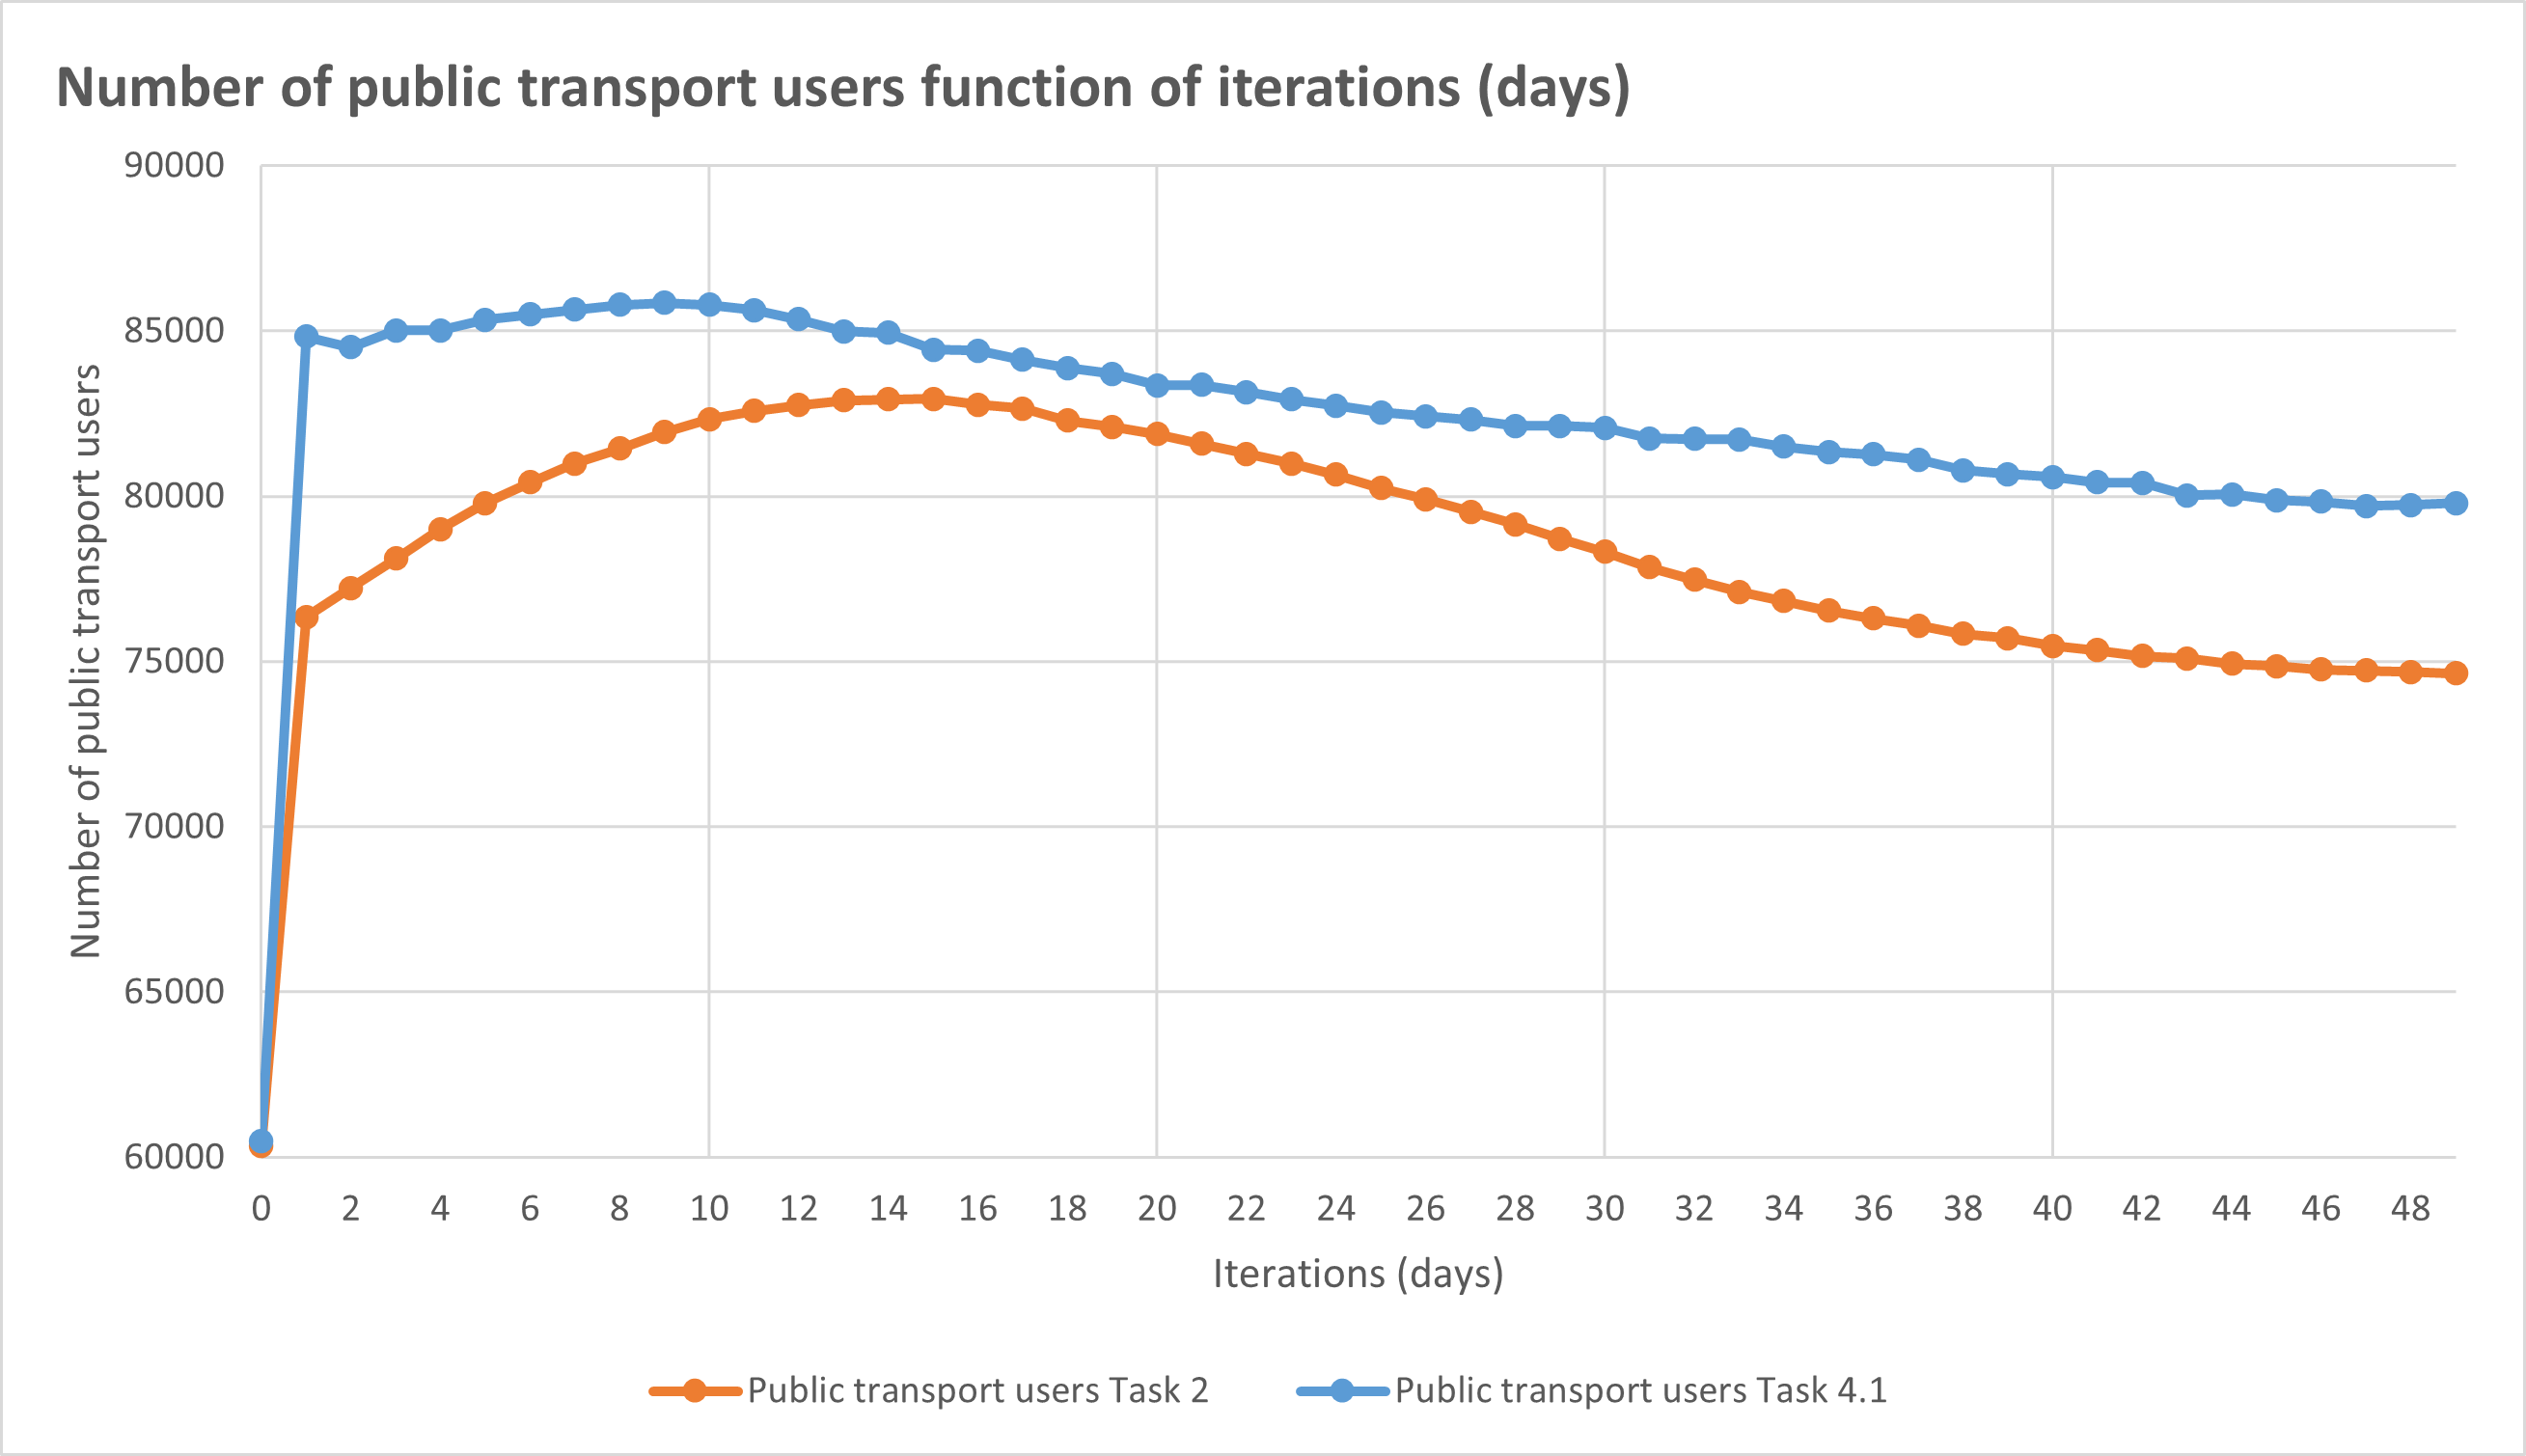
\includegraphics[width=0.8\textwidth]{Images/Step4/number_TP_users_function_iterations_comparaison_task2_4.1.png}
    \caption{Number of public transportation users function of iterations for the task 2 and 4.1 (days)}
    \label{fig:Number of public transportation users function of iterations for the task 2 and 4.1 (days)}
\end{figure}

We notice an initial decrease in drivers in both cases, but a stronger decrease in the toll case. As argued before, this can be explained by the strong initial shift of users to public transport, not wanting to pay and be in traffic jams. Second, we note that the number of drivers remains stable, in contrast to the previous situation where it continued to decrease. In fact, in this new scenario, all the people who could change modes have done so. All that remains are those who want to continue driving to work. Finally, the number of drivers increases again in both cases as congestion is gradually reduced. This strong measure thus exploited the carryover capacity almost to the full, leading to a final situation with a larger share of public transport users (+5128 users).\\











%\begin{minipage}[c]{0.5\textwidth}
%\begin{figure}[H]
%    \centering
%    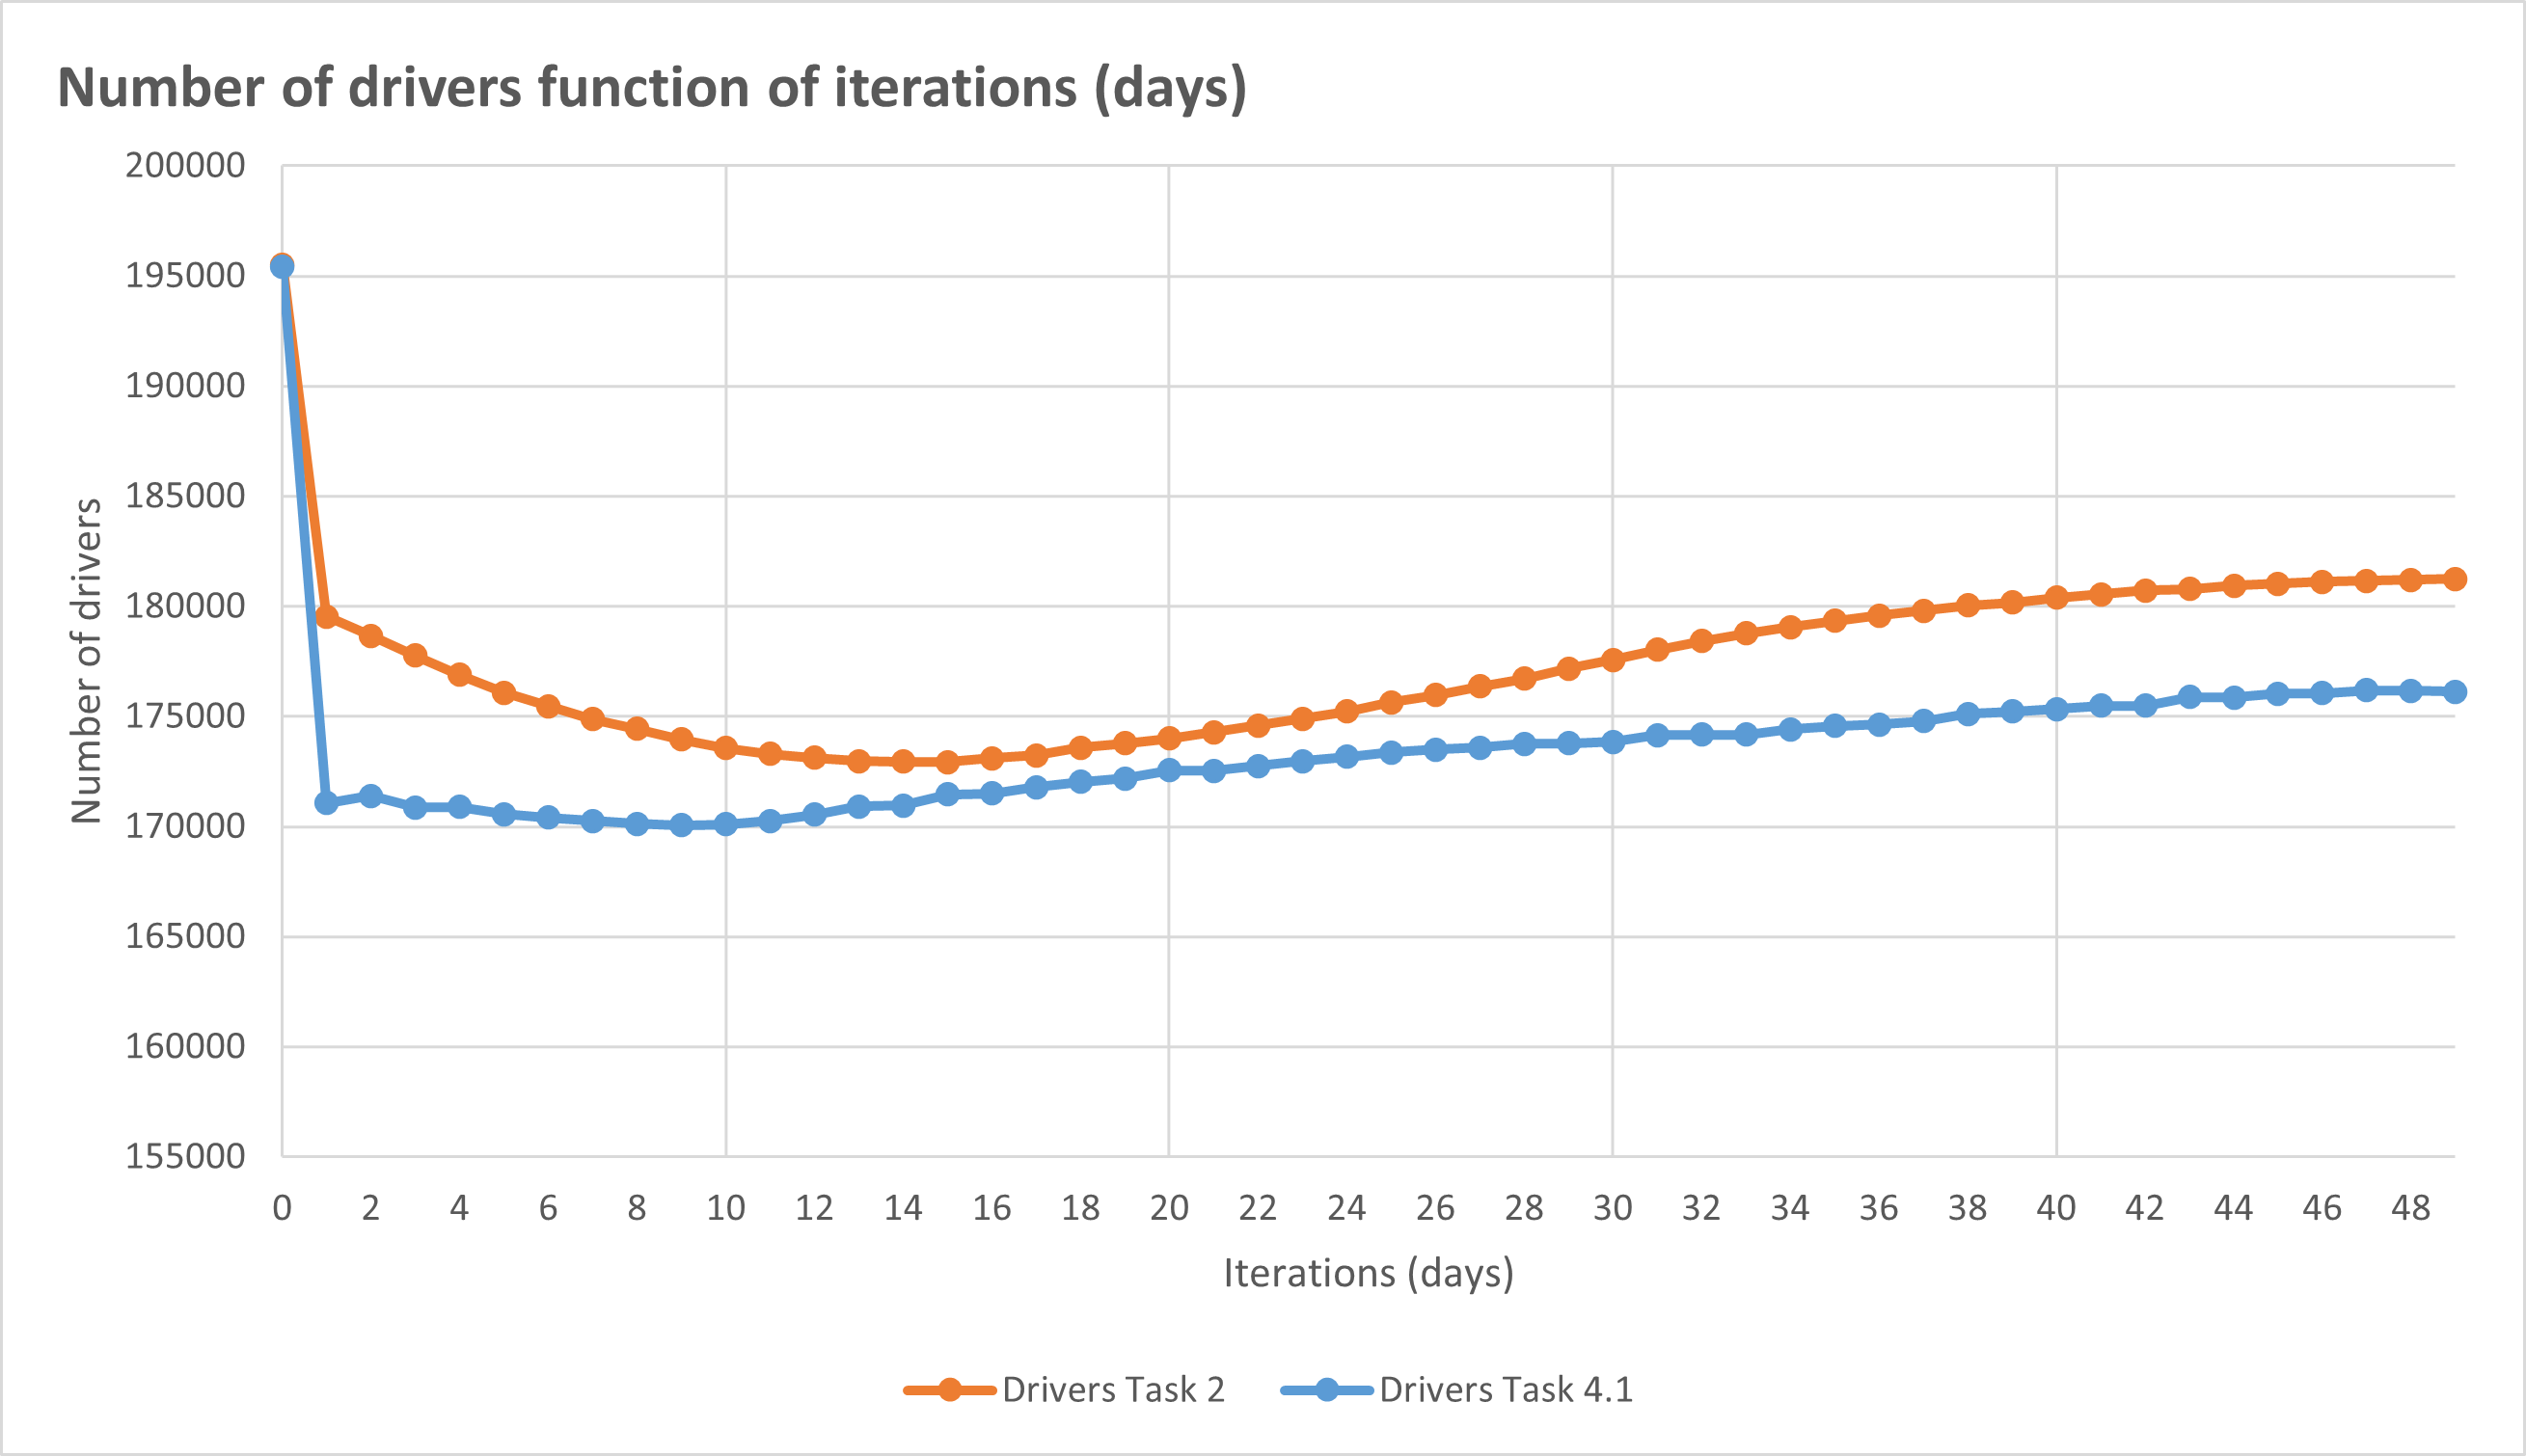
\includegraphics[width=1\textwidth]{Images/Step4/number_drivers_function_iterations_comparaison_task_2_4.1.png}
%    \caption{Number of drivers function of iterations for the task 2 and 4.1 (days)}
%    \label{fig:Number of drivers function of iterations for the task 2 and 4.1 (days)}
%\end{figure}
%\end{minipage}
%\begin{minipage}[c]{0.5\textwidth}
%\begin{figure}[H]
%    \centering
%    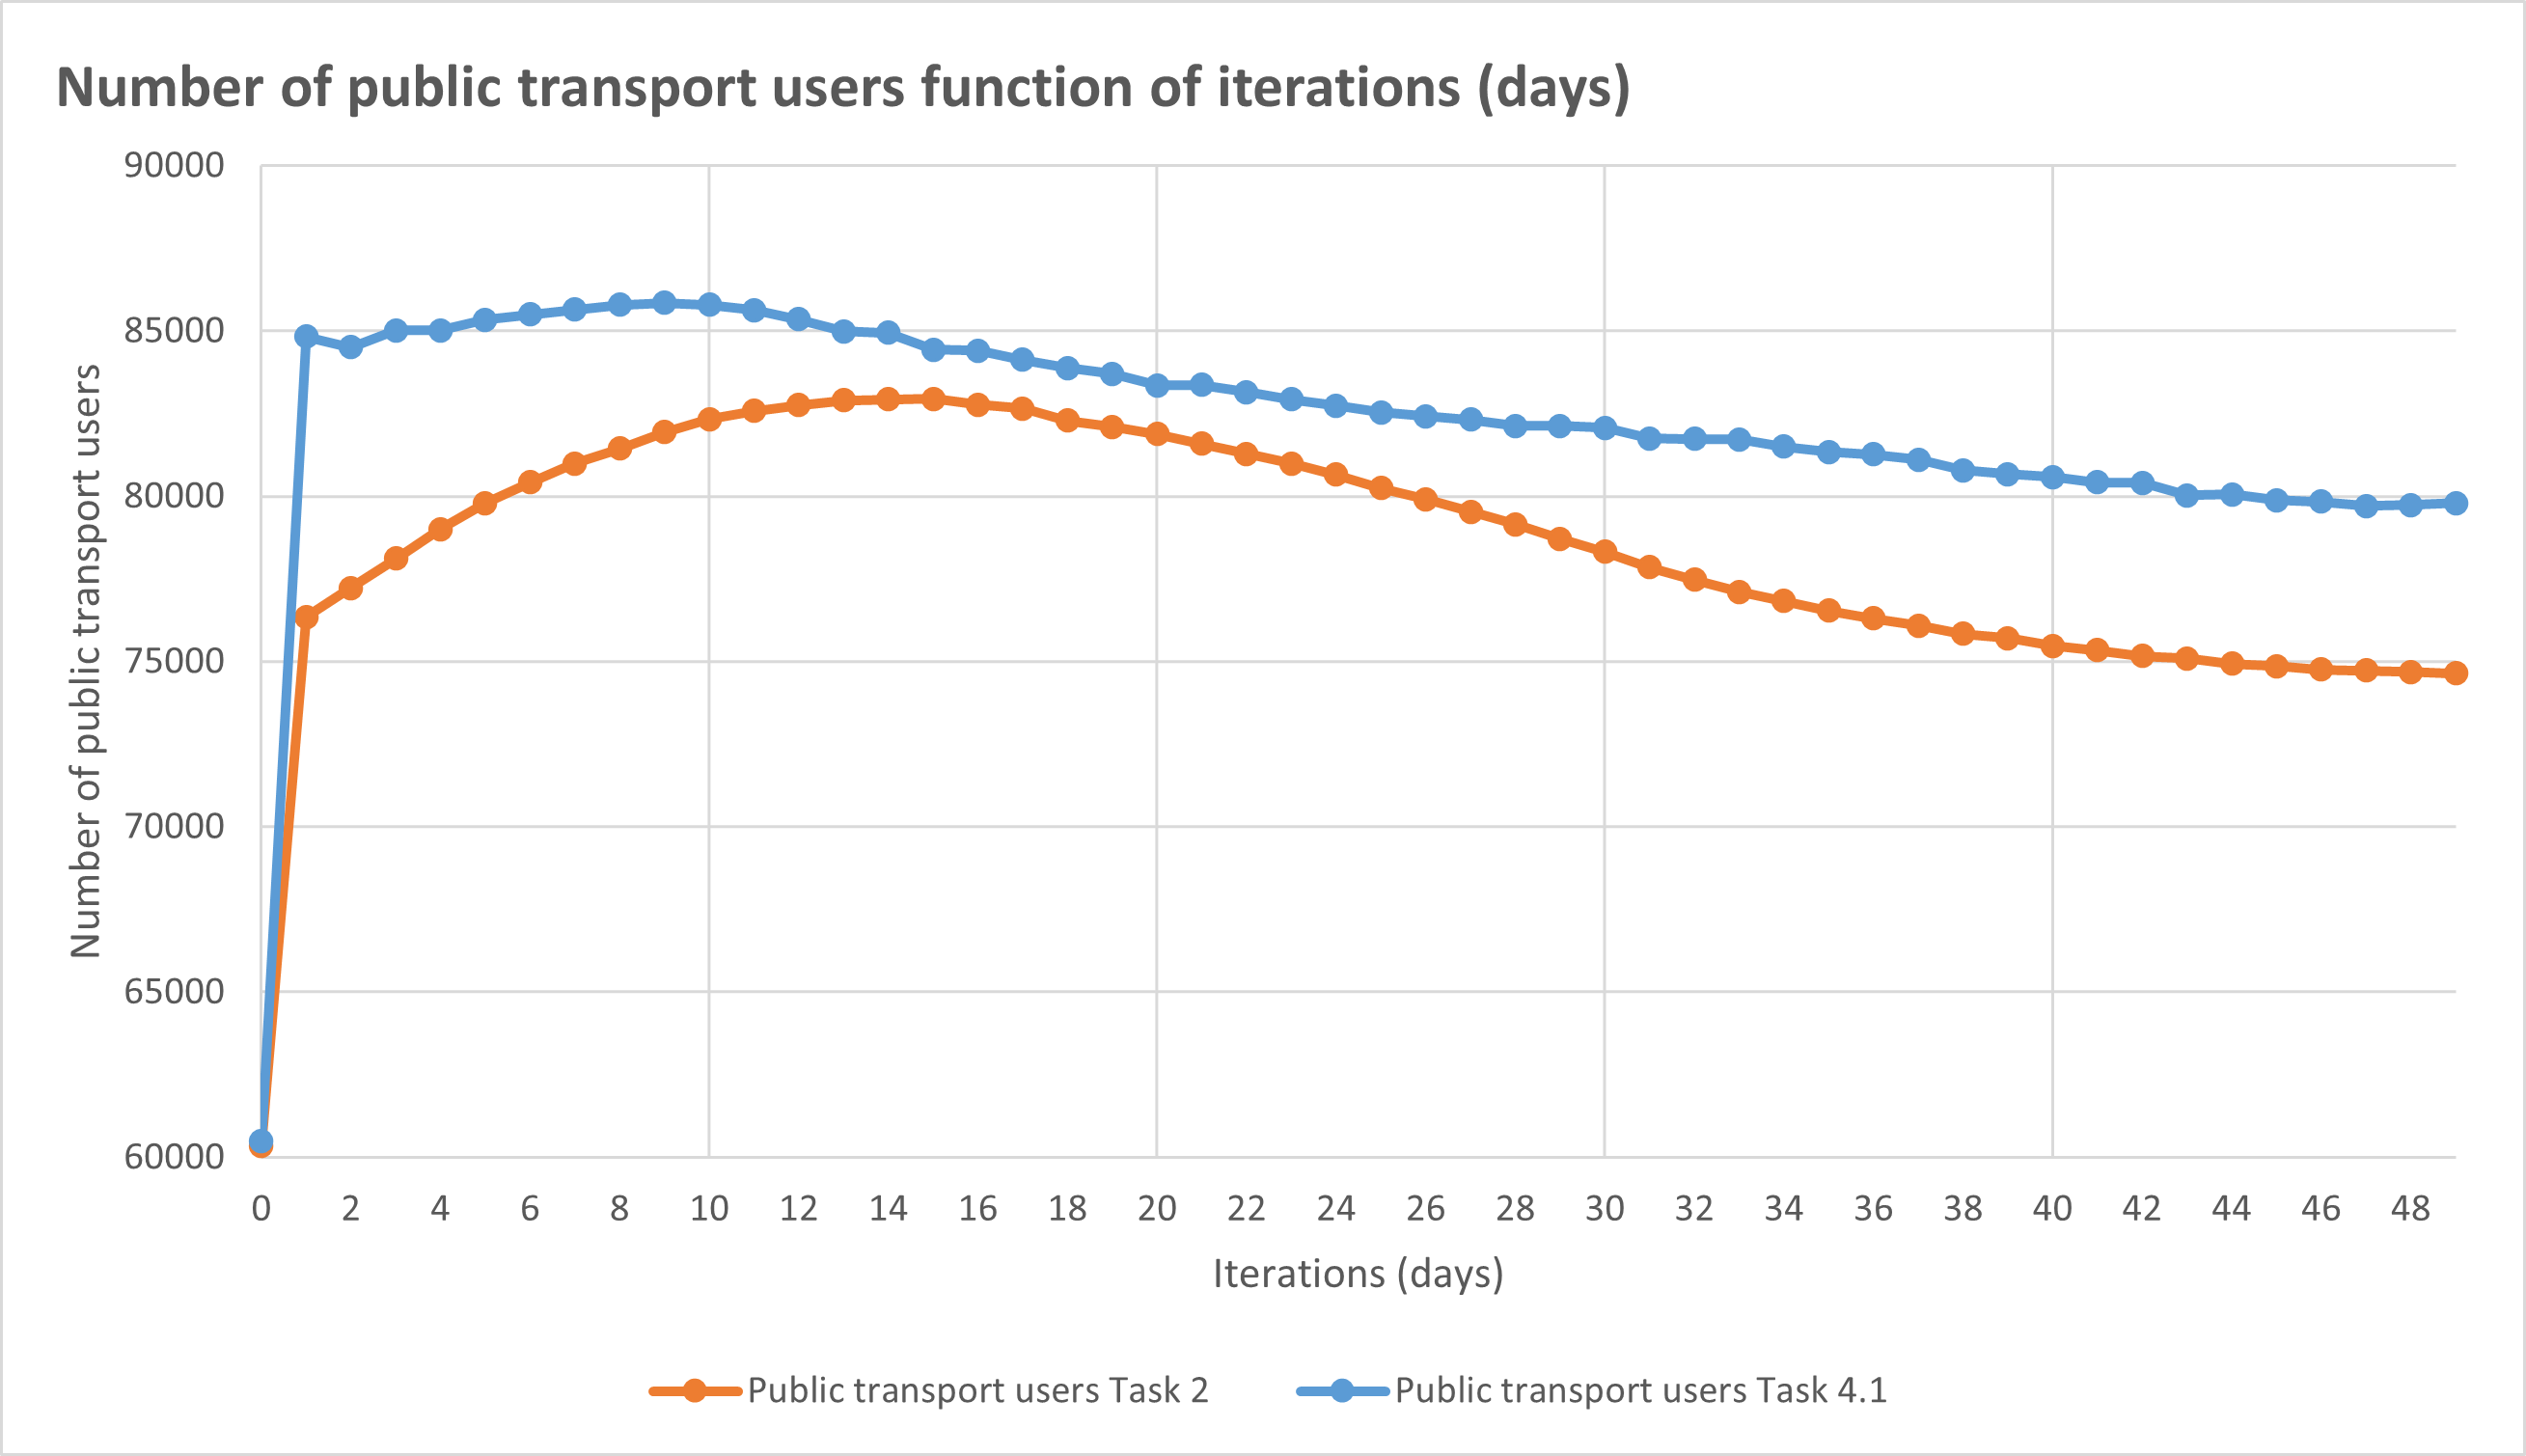
\includegraphics[width=1\textwidth]{Images/Step4/number_TP_users_function_iterations_comparaison_task2_4.1.png}
%    \caption{Number of public transportation users function of iterations for the task 2 and 4.1 (days)}
%    \label{fig:Number of public transportation users function of iterations for the task 2 and 4.1 (days)}
%\end{figure}
%\end{minipage}


Now we can try to compare the situations regarding speeds and travel times.\\

\begin{figure}[H]
    \centering
    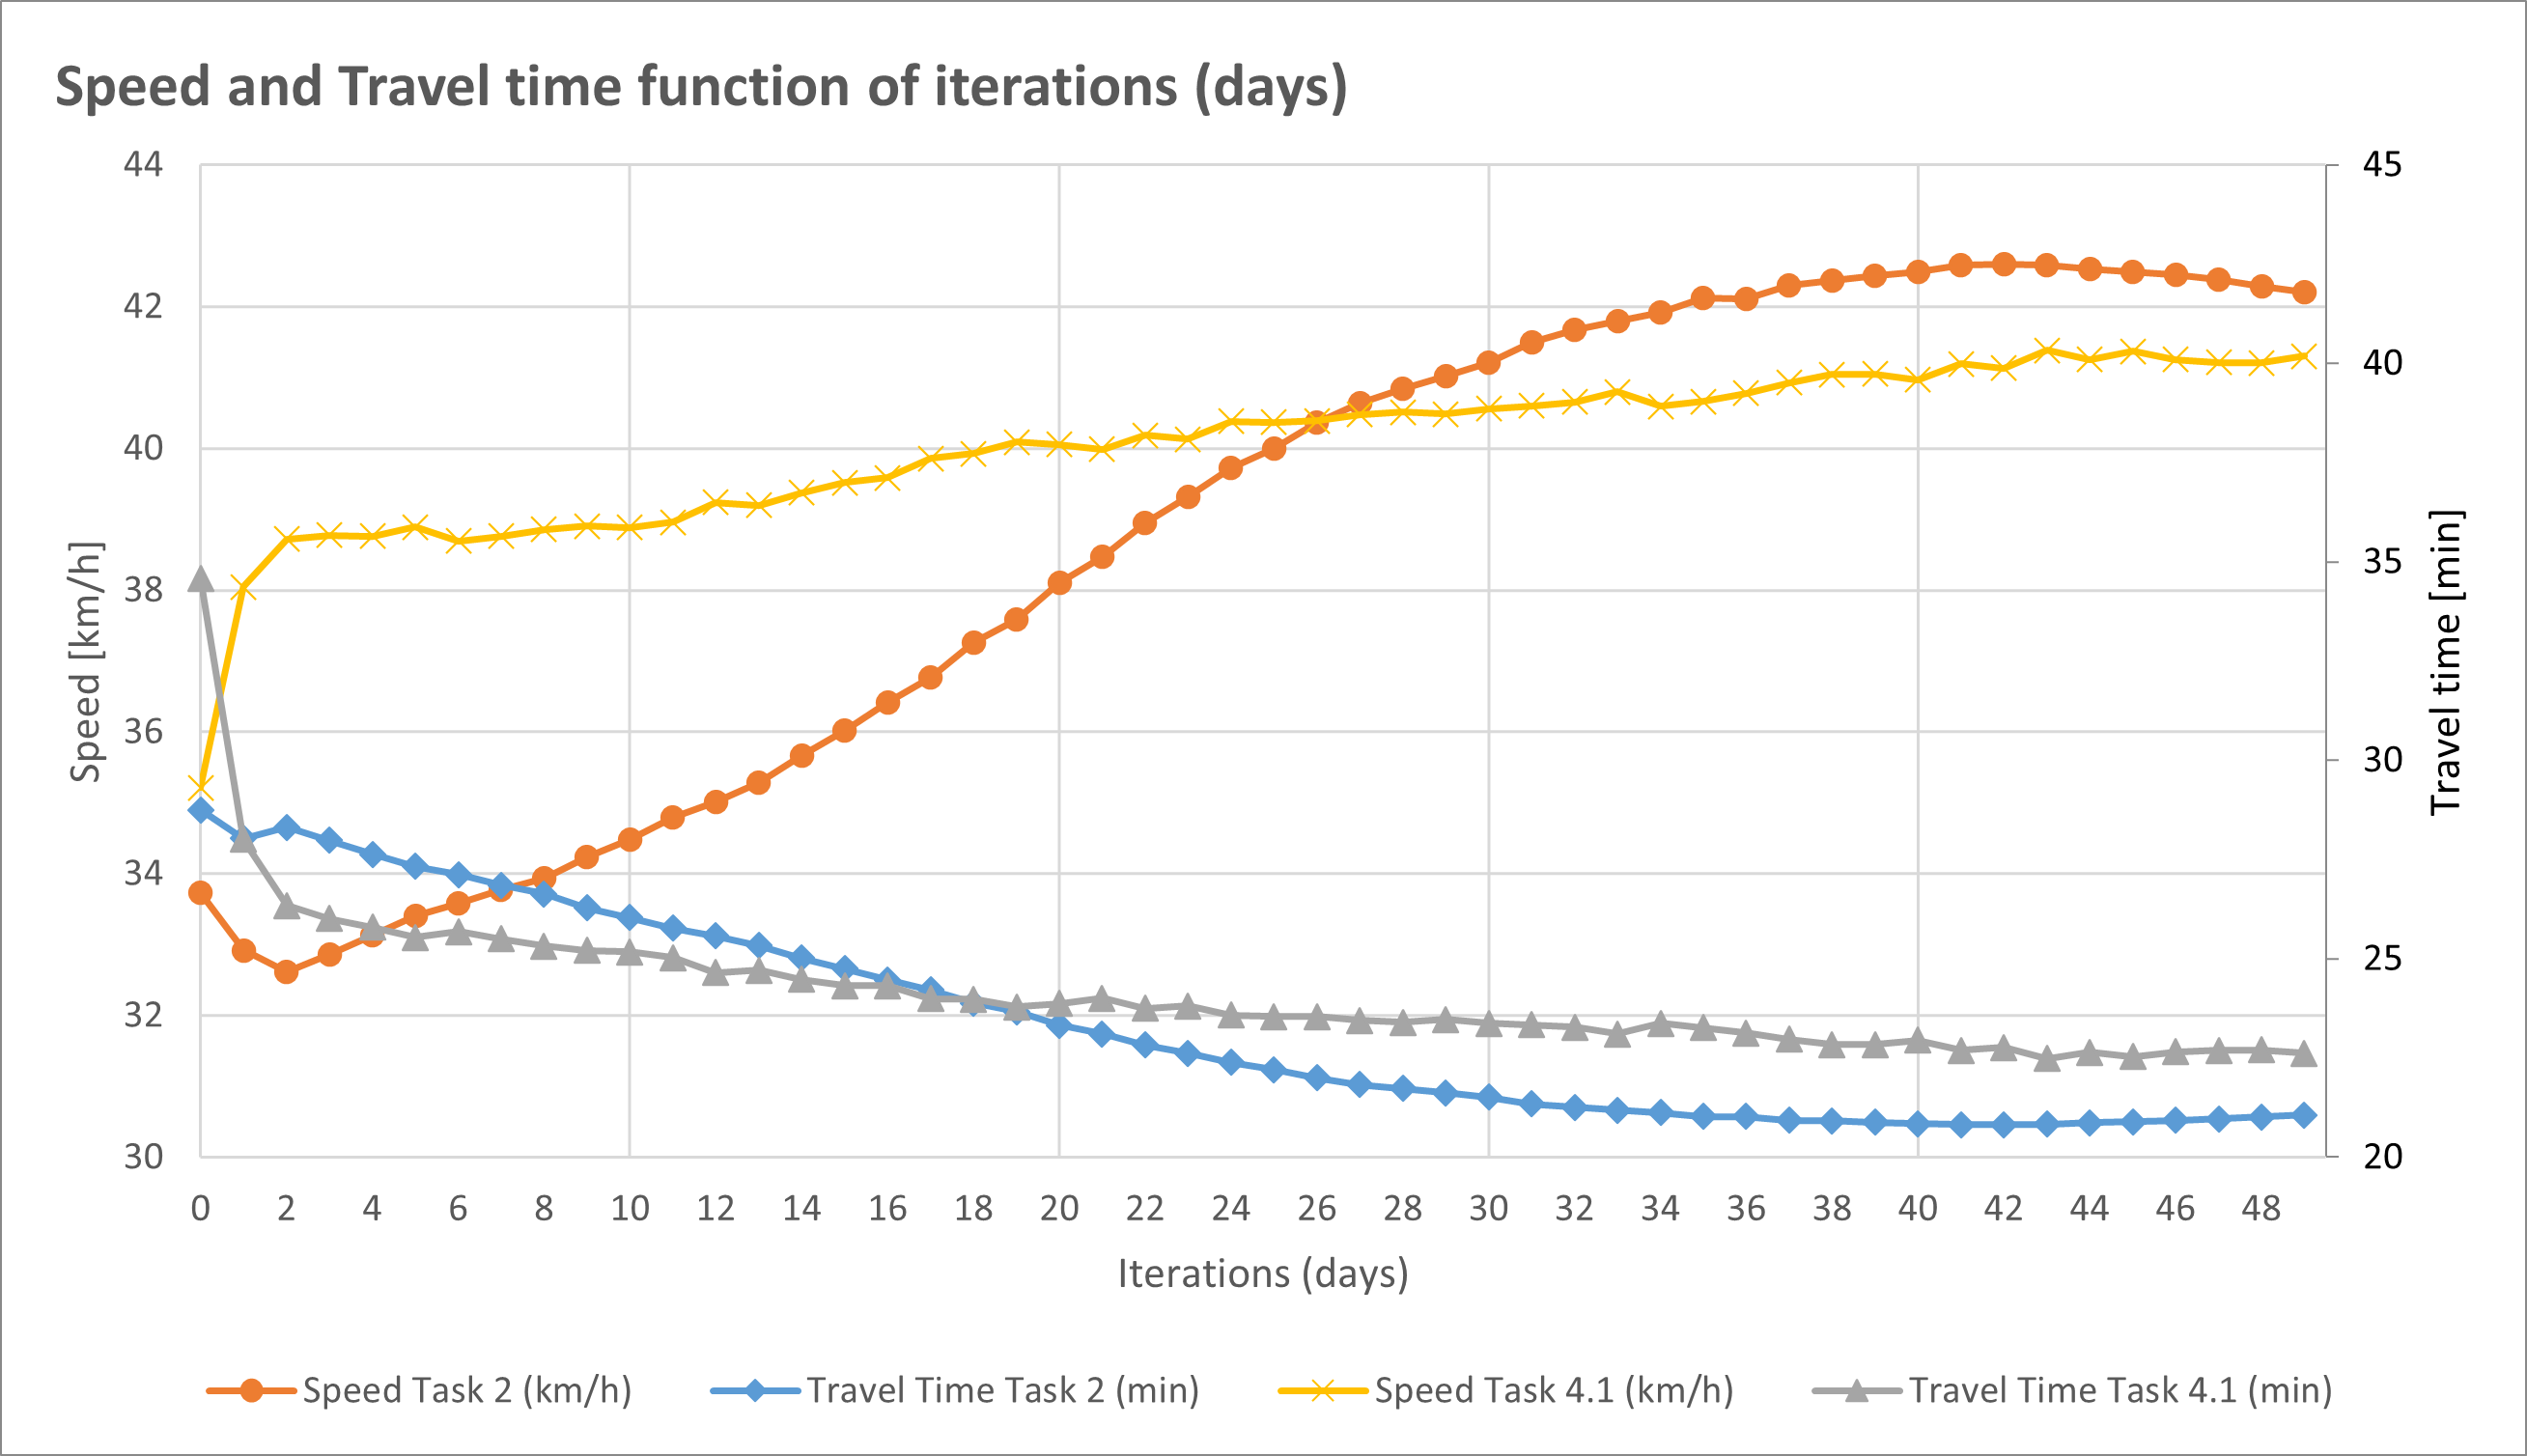
\includegraphics[width=0.8\textwidth]{Images/Step4/Speed_travel_time_function_iterations_comparaison_task_2_4.1.png}
    \caption{Speed and Travel time function of iterations for task 2 and 4.1 (days)}
    \label{fig:Speed and Travel time function of iterations for the task 2 and 4.1 (days)}
\end{figure}

Due to the strong shift of passengers to public transport in the first iterations, we see a strong increase in speed and a drop in travel time. Afterwards, these evolutions continue but much more moderately. This is logical since congestion is decreasing. So speed will increase and the travel time will decrease. We note that these improvements are less rapid in the priced situation than in the first. This may again be the consequence of a smaller variation in the congestion rate.\\

In the end, we have a lower speed (-2.0129 [km/h]) and a higher travel time (1.5582 [min]).\\

Finally, concerning the ratios, we note that the variation is stronger in the first iterations in the new situation than in the previous one. The early arrival rate jumps due to the sudden change in user behaviour, because of the pricing.\\

\begin{minipage}[c]{0.5\textwidth}
\begin{figure}[H]
    \centering
    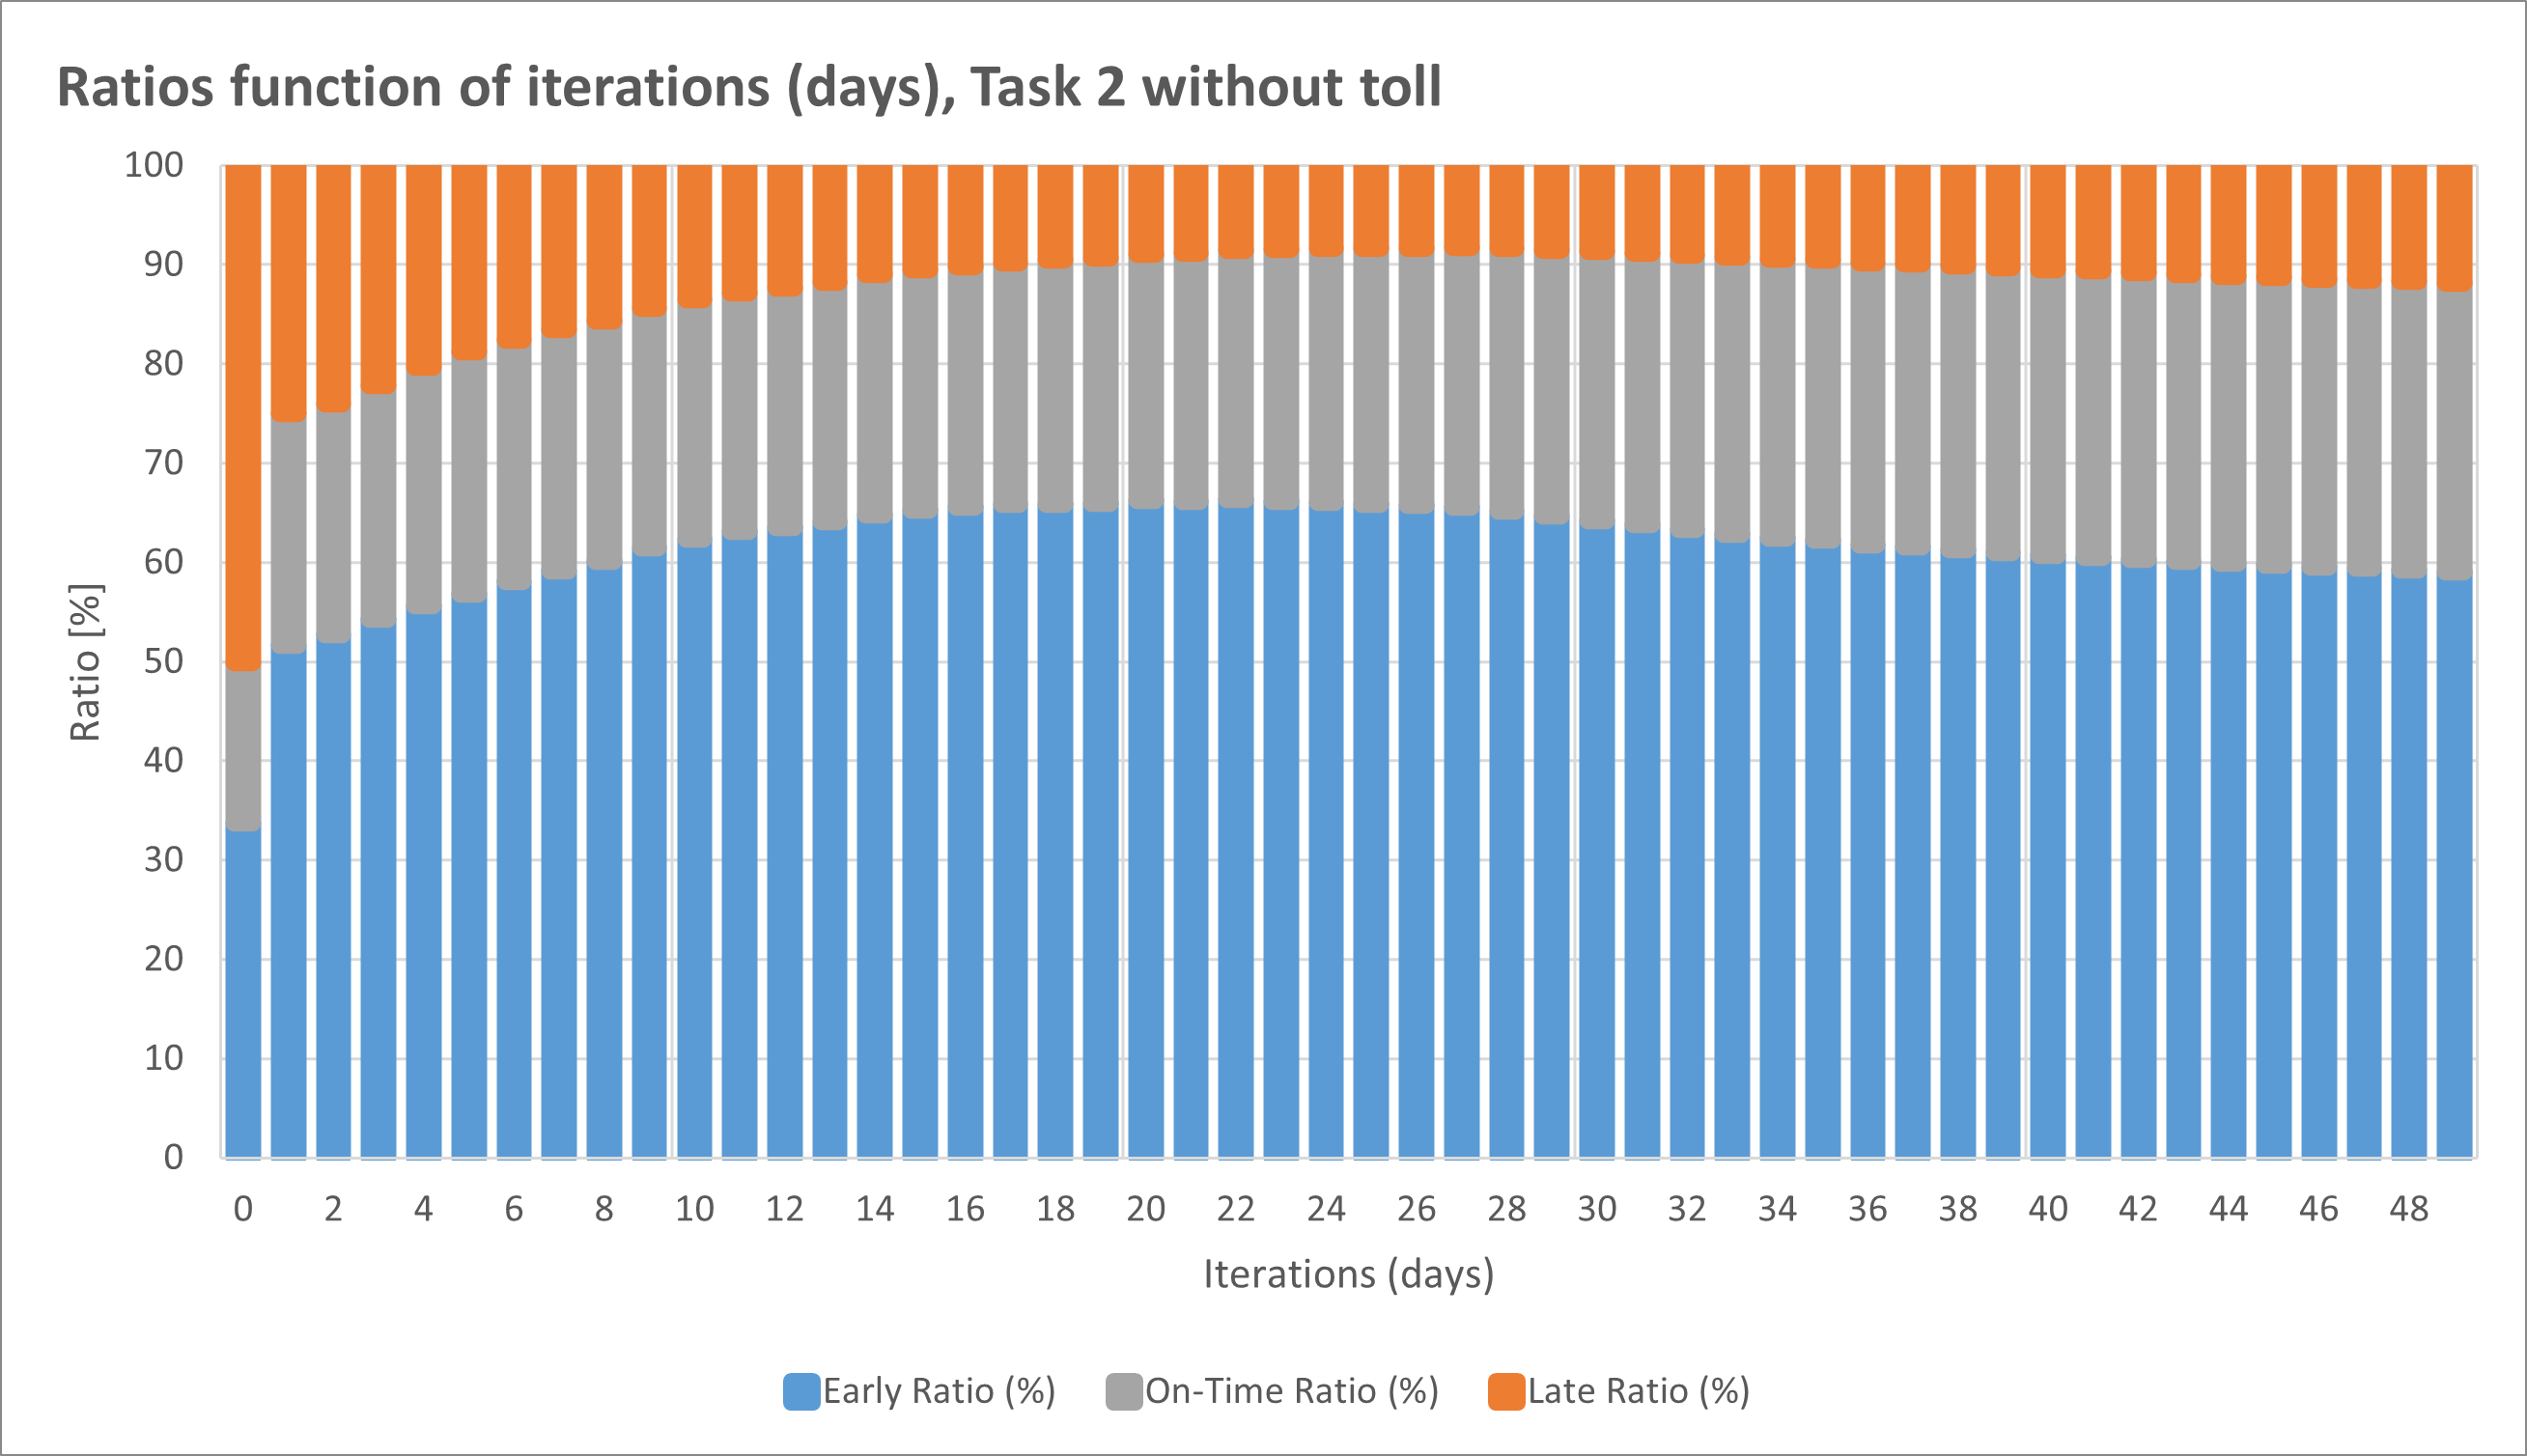
\includegraphics[width=1\textwidth]{Images/Step4/Ratios_function_iterations_comparaison_task_2.png}
    \caption{Ratios function of iterations for the task 2 (days)}
    \label{fig:Ratios function of iterations for the task 2 (days)}
\end{figure}
\end{minipage}
\begin{minipage}[c]{0.5\textwidth}
\begin{figure}[H]
    \centering
    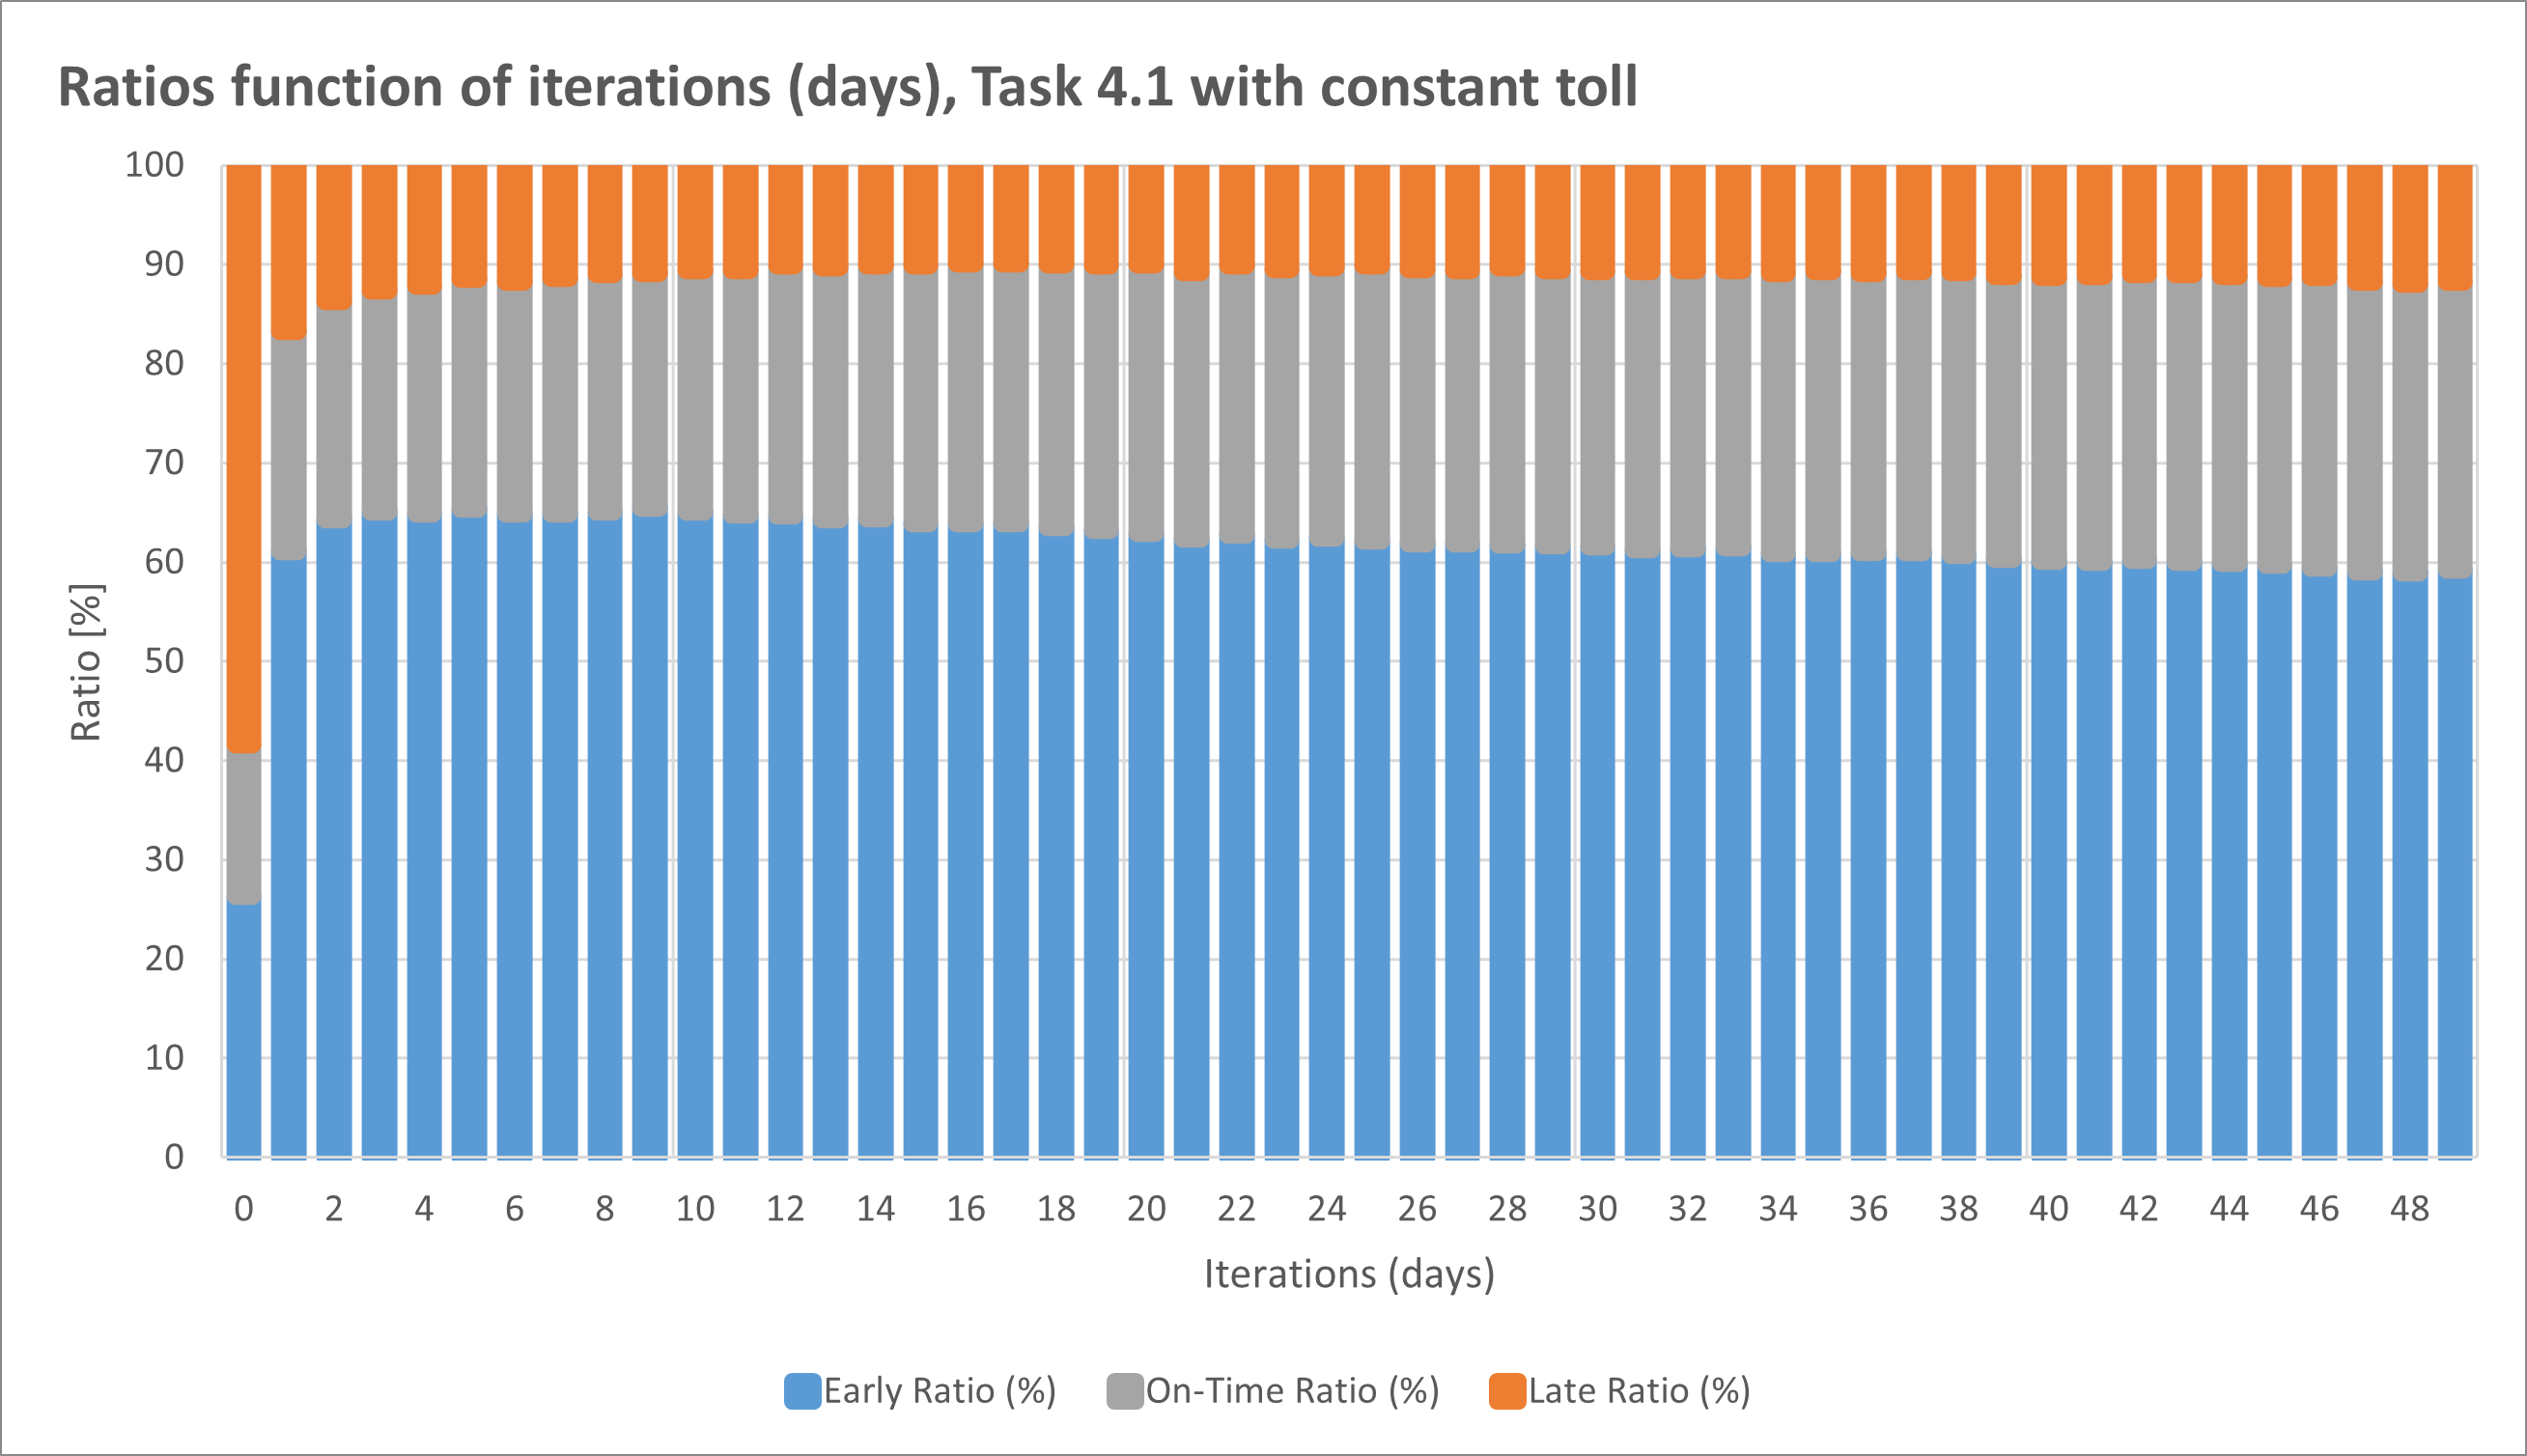
\includegraphics[width=1\textwidth]{Images/Step4/Ratios_function_iterations_task_4.1.png}
    \caption{Ratios function of iterations for the task 4 (days)}
    \label{fig:Ratios function of iterations for the task 4 (days)}
\end{figure}
\end{minipage}
\\

Until the end of the iterations, the trend is about the same (except that the late arrival rate is more stable). In the end, the on-time arrival rate is slightly lower (-0.0655\%), the early arrival rate slightly higher (+0.2076\%) and the late arrival rate slightly lower (-0.1421\%).


\subsubsection{Analysis of the consequences of the toll}
In the end, this policy is not favourable for users. Indeed, there are fewer drivers on the network but there is even more overall congestion and even less consumer surplus. In addition, travel time is even higher and the various ratios hardly change at all.\\

Since all indicators show an unfavourable trend, this road-pricing policy is not desirable. It is not desirable to have such a road pricing policy, because it provokes opposition from users to the tolls. They will find it more difficult to leave early and still pay the same amount, or they will be tempted to arrive at the inner belt just as the toll is lifted. This is absolutely undesirable since it concentrates the users instead of spreading them over the morning peak period. In the second part, we will propose an alternative to improve the situation.


\subsection{Implementation of the alternative road pricing policy}
During the second part of this task, alternative road pricing policies will be implement in the model. The goal is to characterize the impact of such policies on congestion, the customer surplus and the number of public transportation users. We will compare the result to the global percentage of congestion, but to obtain a more precise overview of the effect, the evolution of congestion over the day will also be analysed. 
The pricing model used is a cordon toll for the links that enter the city center from the first ring and the analysis of congestion will focus on these links to catch the direct effects of the road pricing policy.
Below are the graphs of the evolution of the (relative) additional travel time as a function of the study hours for the cases without tolls and with a constant toll:

\begin{minipage}[c]{0.5\textwidth}
\begin{figure}[H]
    \centering
    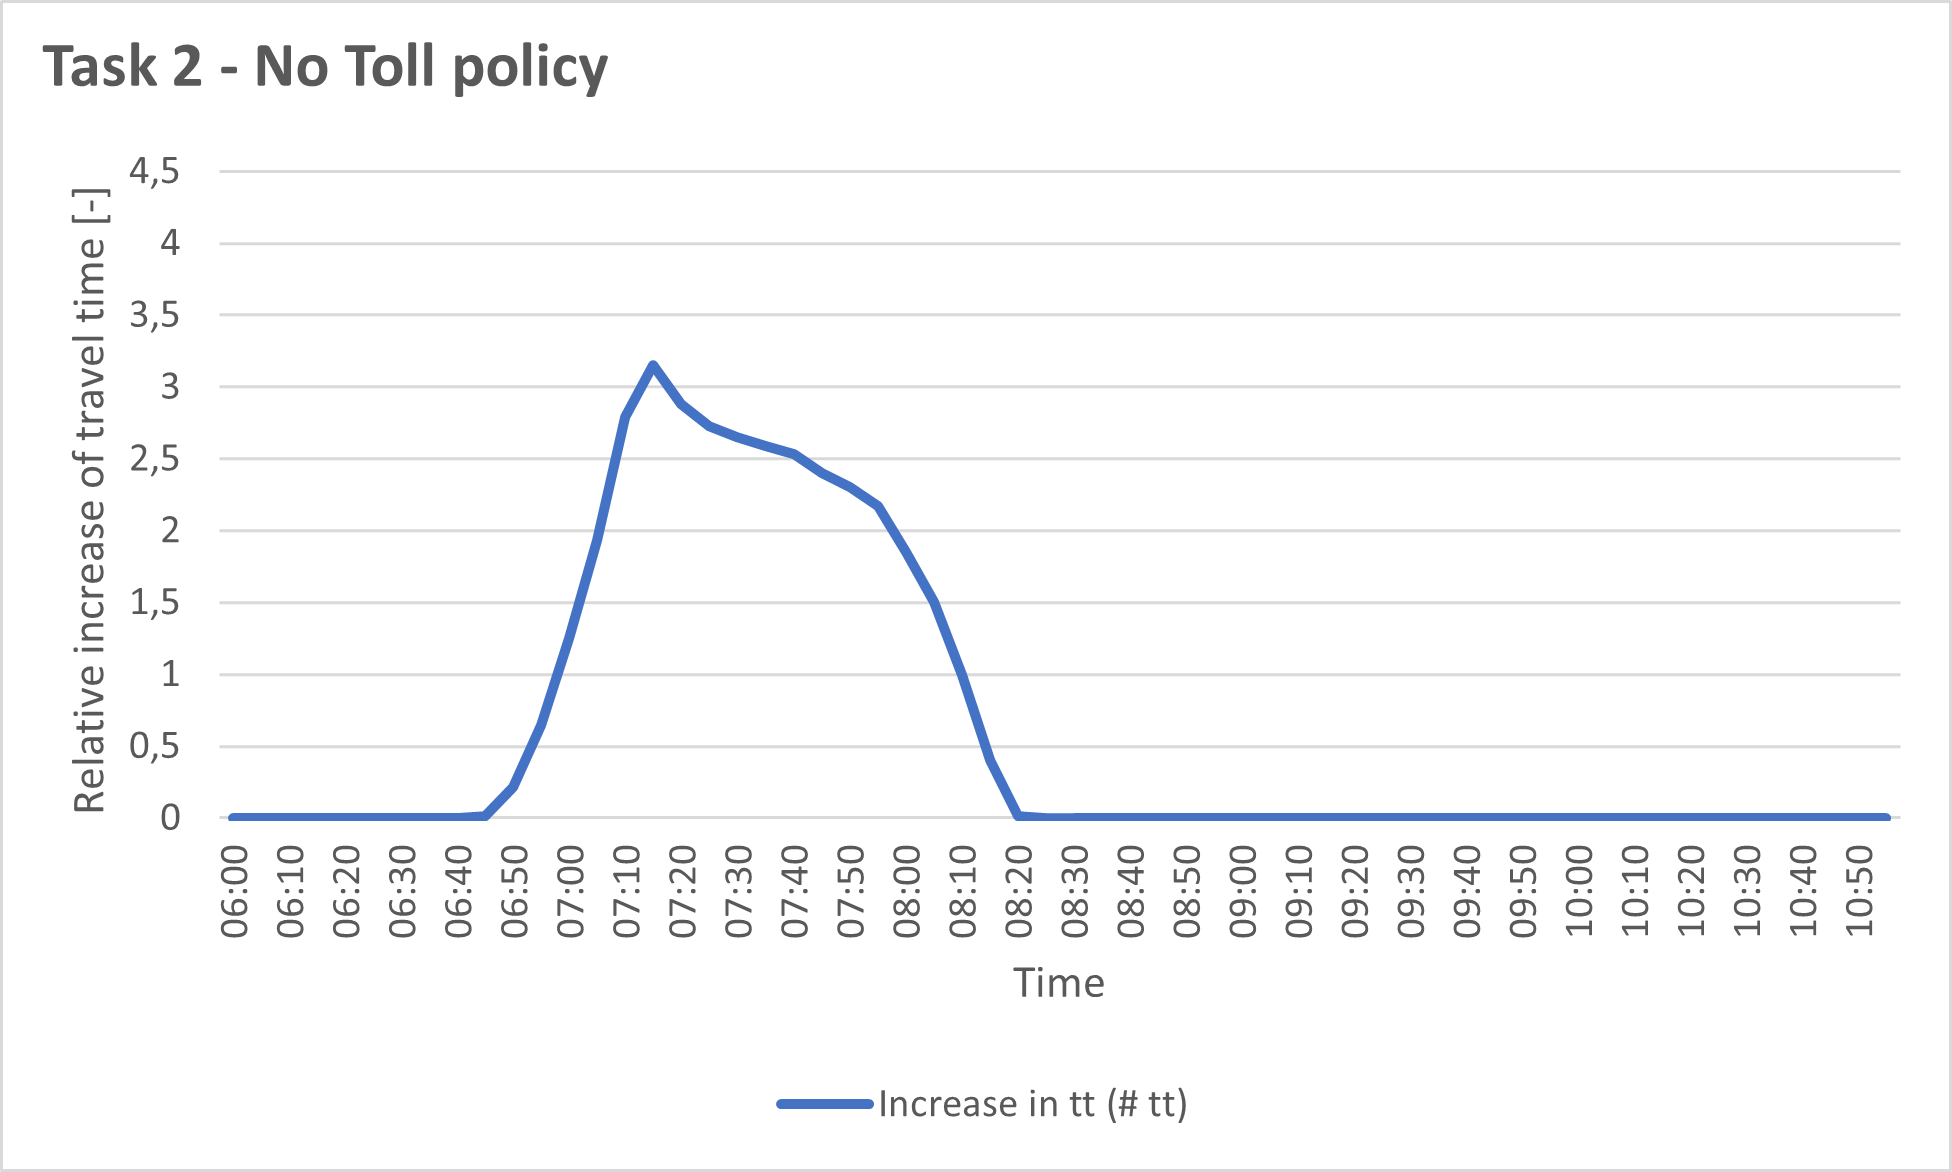
\includegraphics[width=1\textwidth]{Images/Step4/Task4.2_No_Toll_policy.png}
    \caption{Relative increase of travel time without any pricing policy function of the time}
    \label{fig:Relative increase of travel time without any pricing policy function of the time}
\end{figure}
\end{minipage}
\begin{minipage}[c]{0.5\textwidth}
\begin{figure}[H]
    \centering
    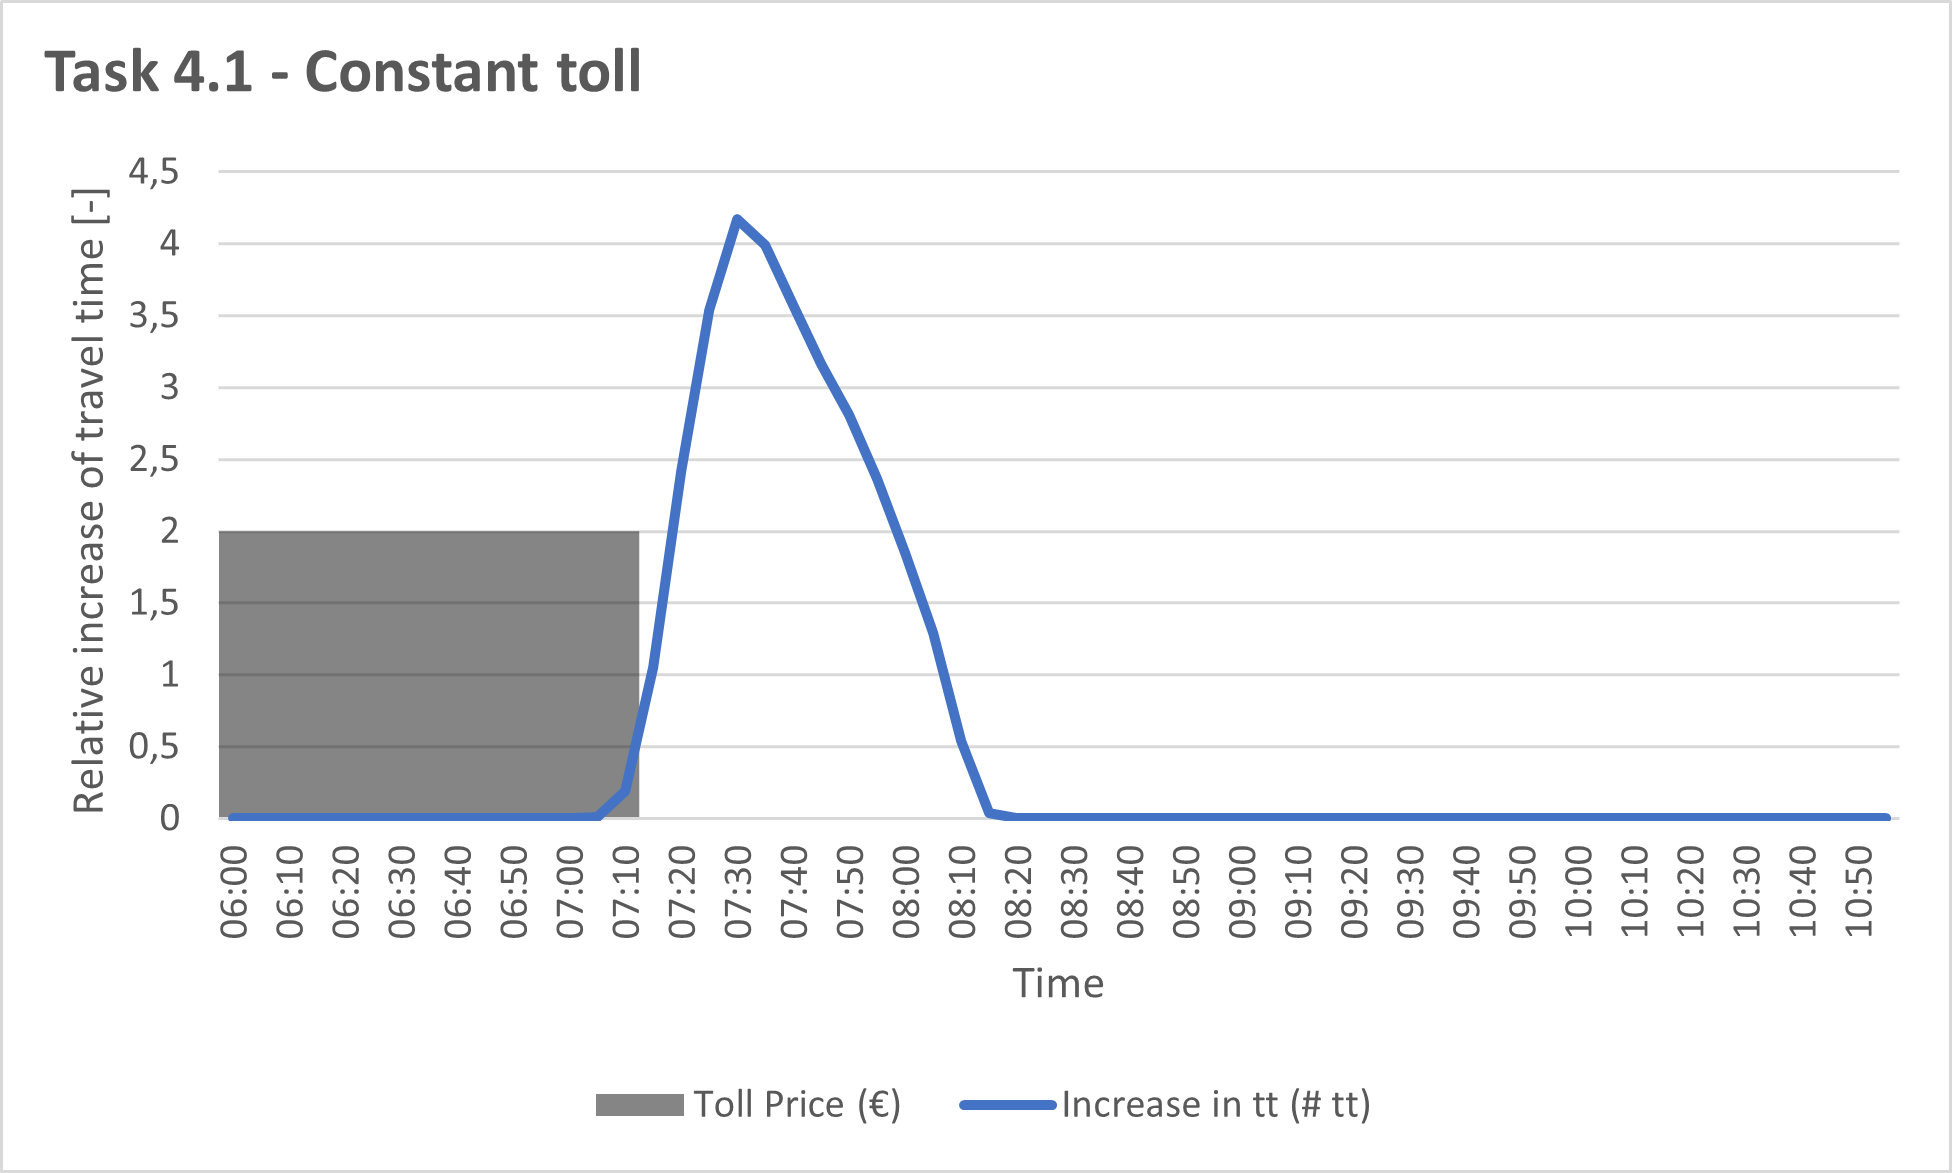
\includegraphics[width=1\textwidth]{Images/Step4/Task4.2_constant_toll.png}
    \caption{Relative increase of travel time with the constant toll model function of the time}
    \label{fig:Relative increase of travel time with the constant toll model function of the time}
\end{figure}
\end{minipage}
\newline

The level of congestion is represented by the increase in travel time compared to the baseline travel time observed in the absence of congestion. The unit of the graph is the number of additional basic travel times. Thus, when the value is 1, the travel time at that point in time on all links entering the city centre is 100\% longer than the expected travel time in the absence of congestion.\\
In the situation without a tolling strategy, peak congestion occurs between 7:15 am and 7:20 am with a relative increase of over 300\% compared to the uncongested hours.\\
In the situation with a constant toll (Task 4.1), the peak is between 7:30 am and 7:35 am with an increase of more than 400\%. On the basis of the shape of this graph, we can understand the comments made in the previous section, particularly with regard to the delayed departures from home and therefore the delayed arrival at the inner ring road. The graphs shown show this clearly.\\

The method we have followed is to study different types of pricing strategies and compare them so that we can select the most conclusive one and analyse it in more detail. Different pricing policies will therefore be implemented to reduce and mitigate the level of congestion during peak hours. They are listed in the following figure:

\begin{figure}[H]
    \centering
    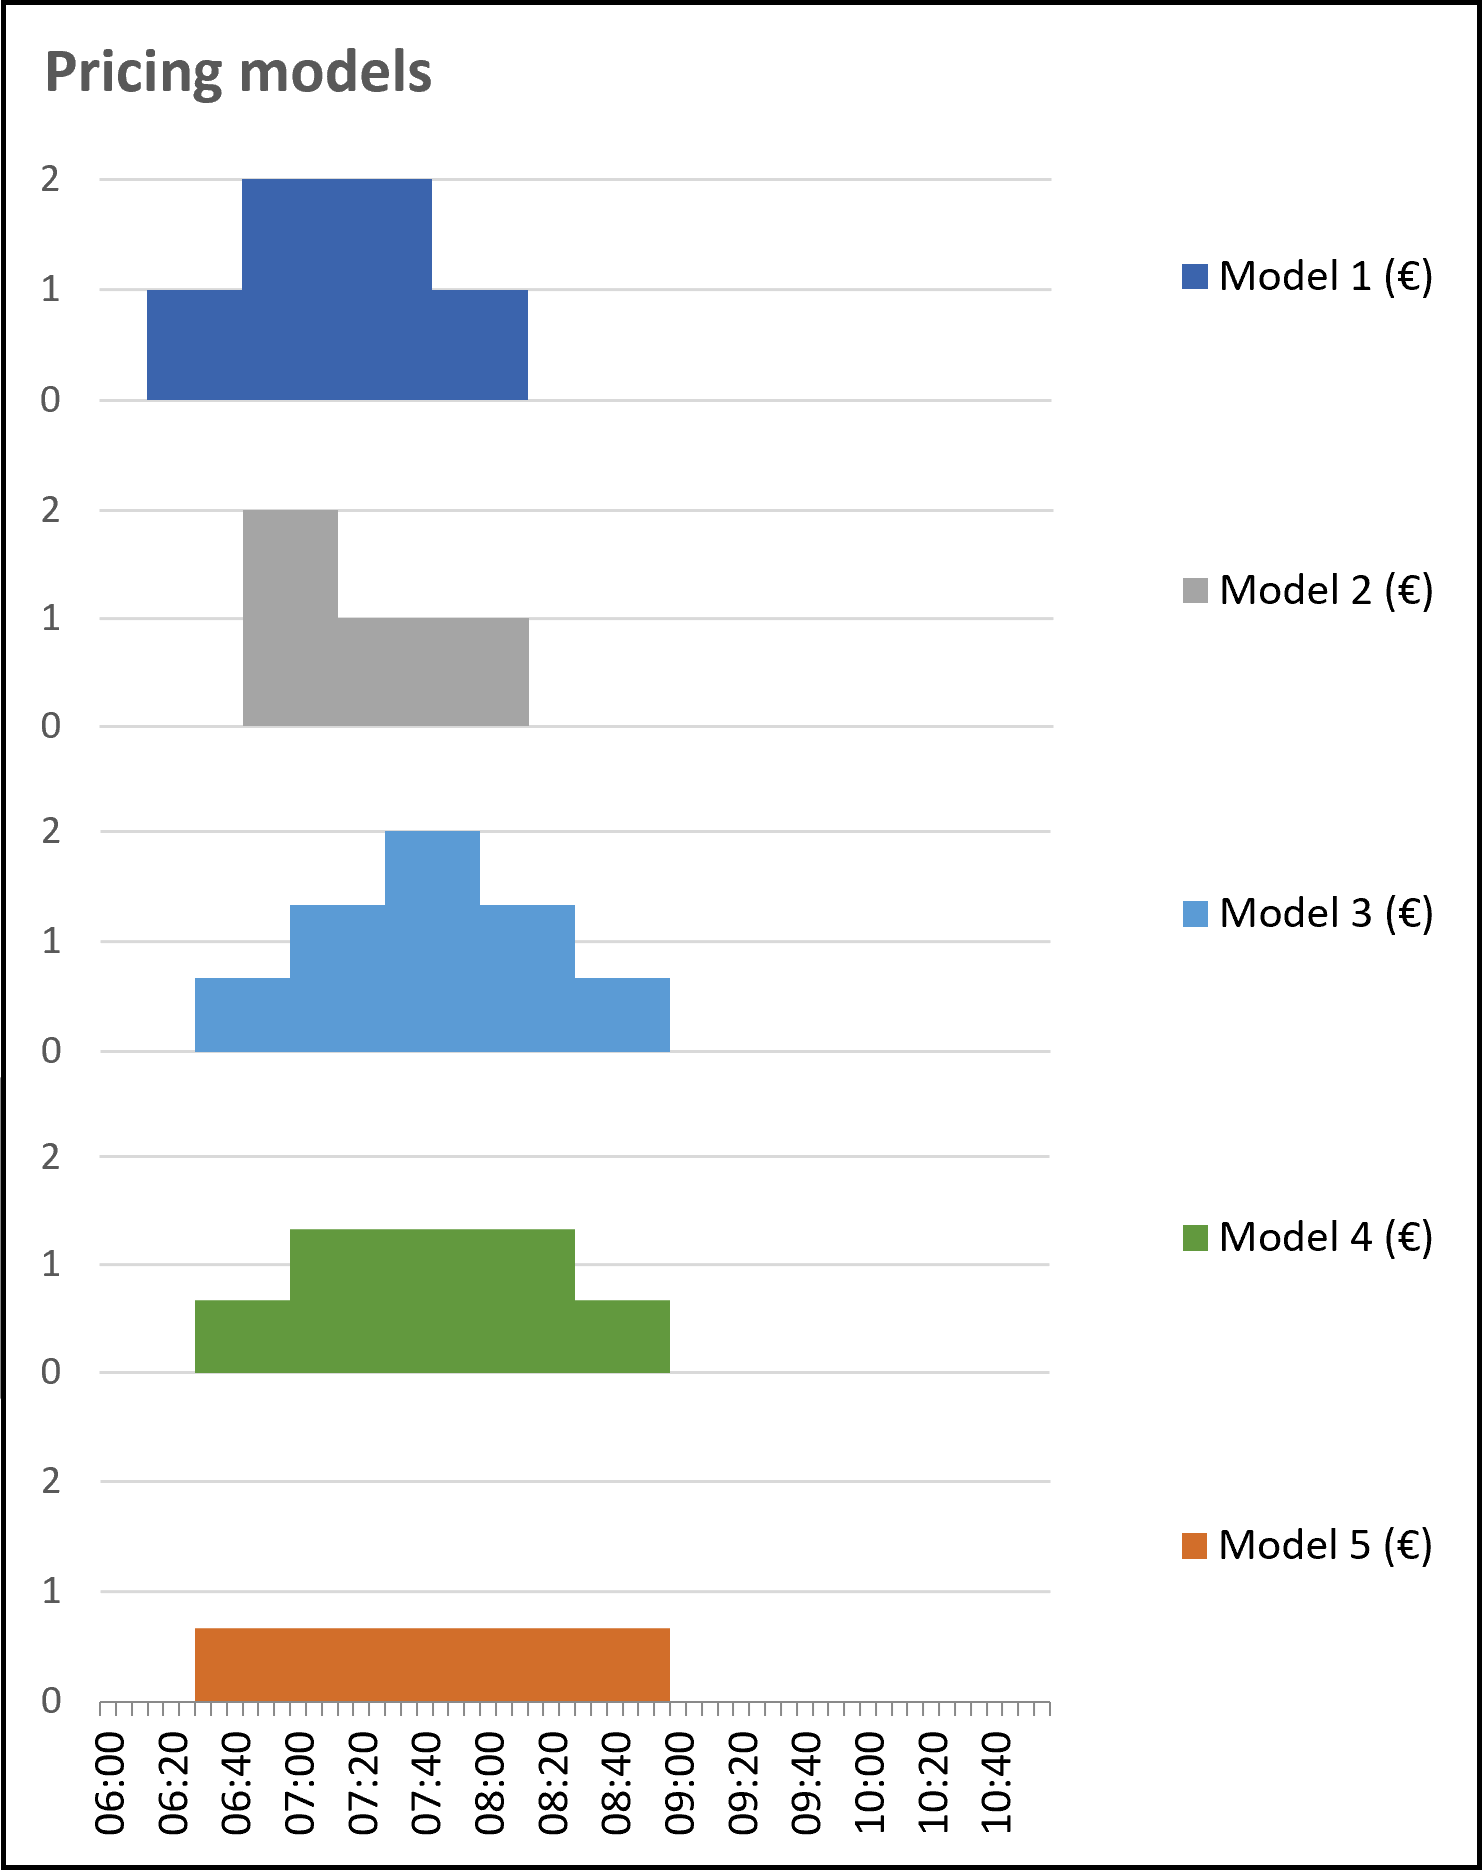
\includegraphics[width=0.5\textwidth]{Images/Step4/Pricing policies.png}
    \caption{Models of pricing policy}
    \label{fig:Models of pricing policy}
\end{figure}

The first model is a two levels pricing policy with a 2€ toll between 6:45 am and 7:45 am, and a 1€ toll 30 minutes before and after. This shape of pricing fits the congestion curve and will try to shift some trips before or after the peak hours.\\

The second model is a two levels pricing policy with a 2€ toll between 6:45 am and 7:15 am, and then a residual 1€ toll until 8:15 am. The objective behind this policy is to avoid the quick increase of congestion between 6:45 am and 7:15 am, and then to smooth the level of congestion by keeping a toll until the end of the initial congestion period. What is desired is for drivers to arrive in the city centre before or after rush hour.\\

The third model is a three levels pricing policy with a shape similar to the first model. The maximum toll price for this model is 2€. The width of each step is 30 minutes and the maximal toll happens between 7:30 am and 8:00 am. This model will show how the simulation is responding to an addition of pricing level.\\

The last two models are a copy of model 3, with each time a pricing level removed. The goal of these models is to understand more exactly how model 3 works.

\subsubsection{Results on the network}

First, we will compare the different simulation results following the introduction of each of these road pricing strategies. The results in terms of relative increase in travel time are shown below:

\begin{minipage}[c]{0.5\textwidth}
\begin{figure}[H]
    \centering
    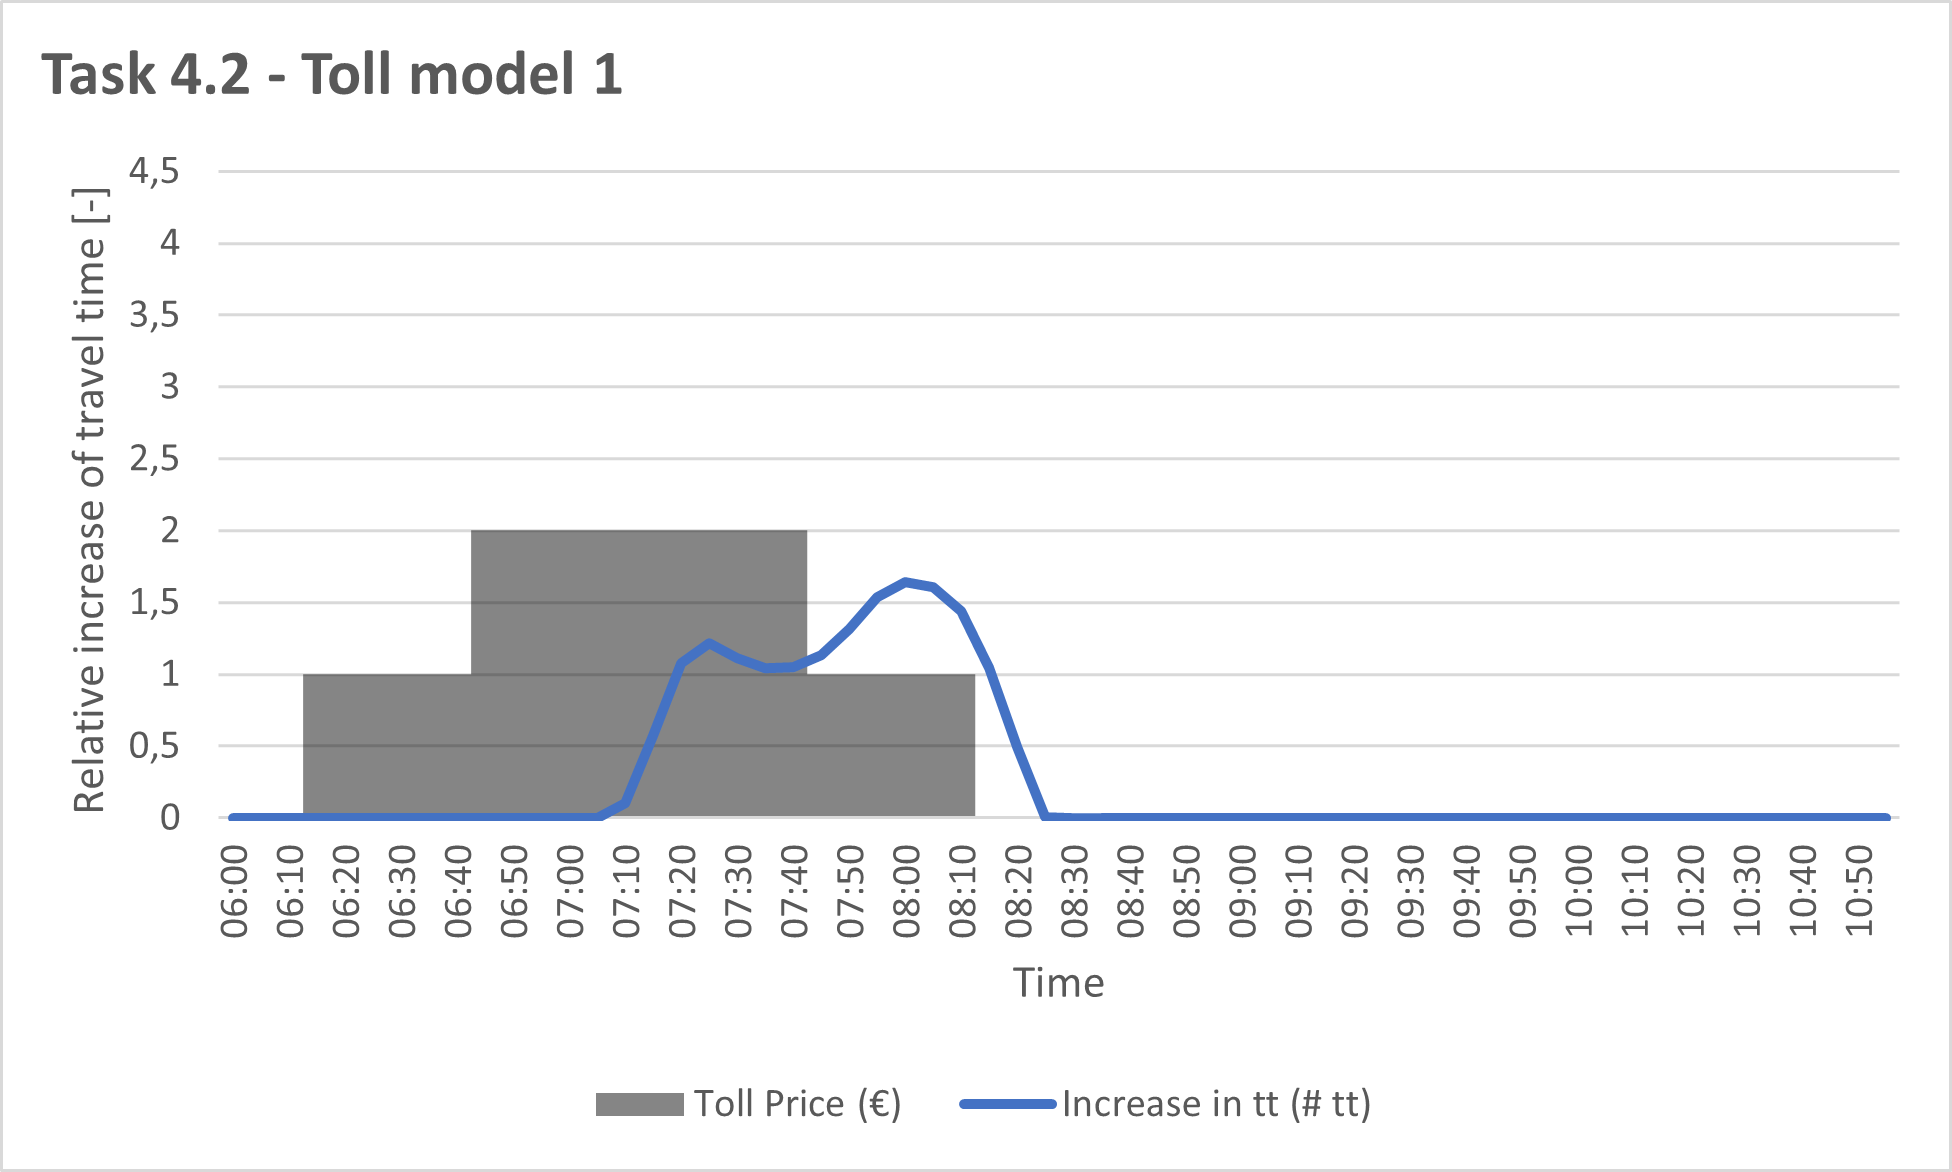
\includegraphics[width=1\textwidth]{Images/Step4/Task4.2_Toll_model_1.png}
    \caption{Relative increase of travel time with toll model 1 function of the time}
    \label{fig:Relative increase of travel time with toll model 1 function of the time}
\end{figure}
\end{minipage}
\begin{minipage}[c]{0.5\textwidth}
\begin{figure}[H]
    \centering
    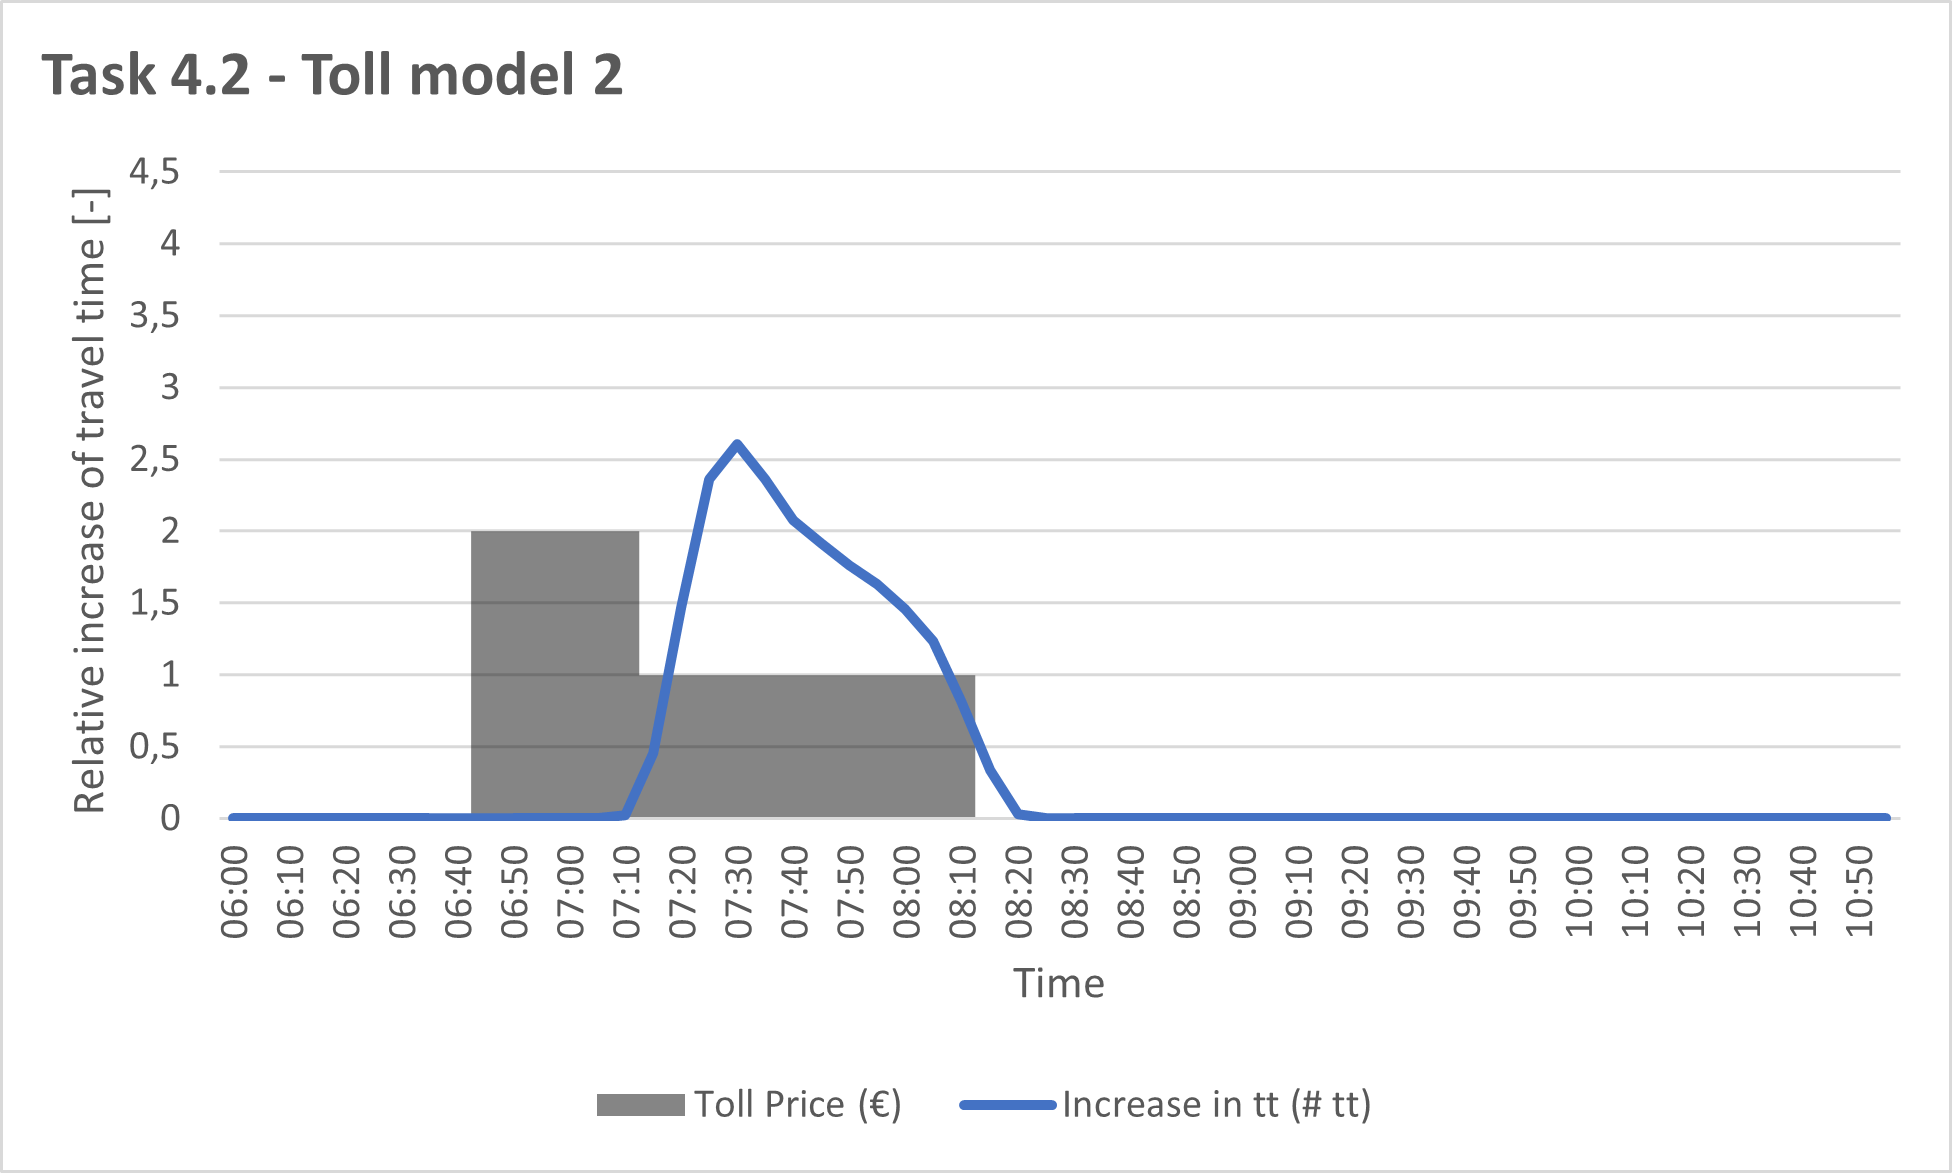
\includegraphics[width=1\textwidth]{Images/Step4/Task4.2_Toll_model_2.png}
    \caption{Relative increase of travel time with toll model 2 function of the time}
    \label{fig:Relative increase of travel time with toll model 2 function of the time}
\end{figure}
\end{minipage}
\begin{minipage}[c]{0.5\textwidth}
\begin{figure}[H]
    \centering
    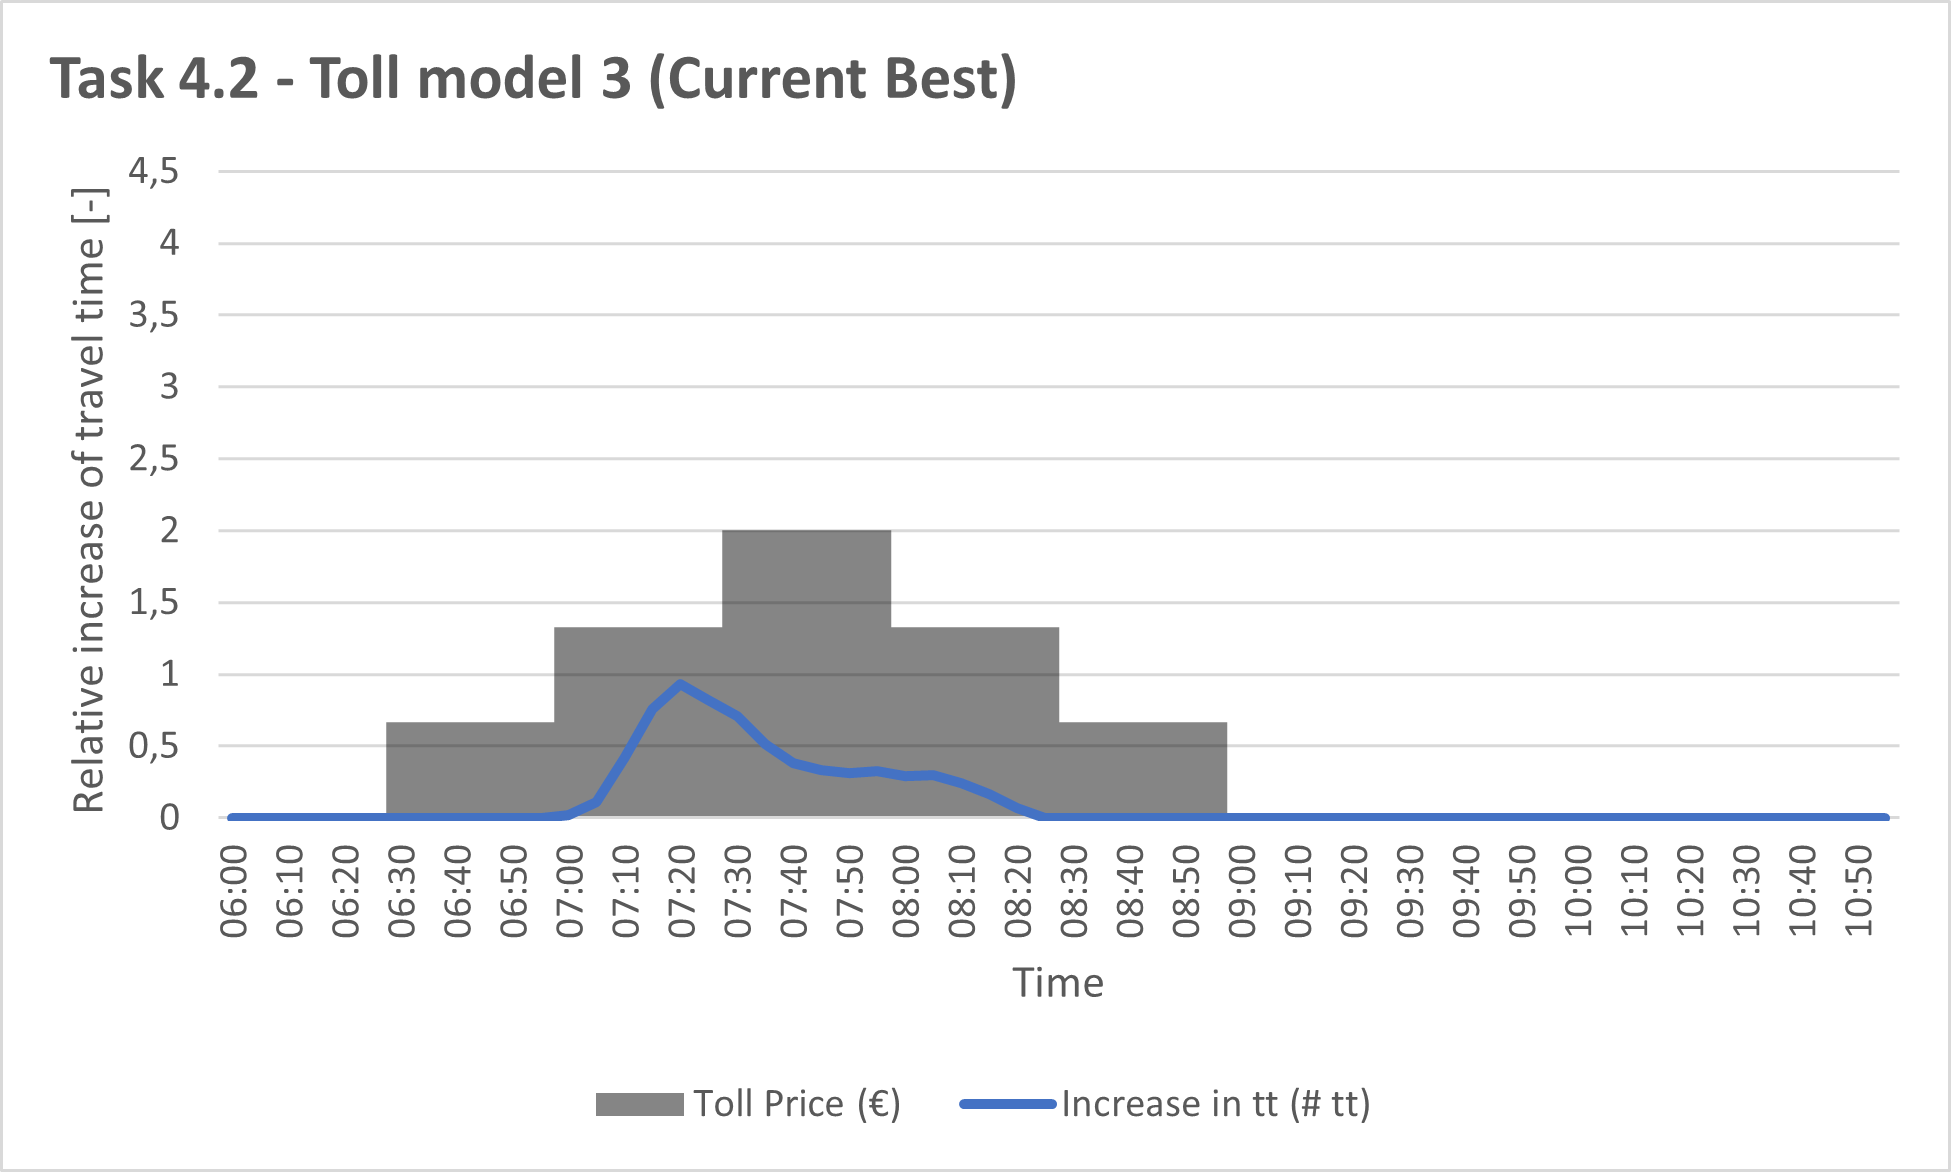
\includegraphics[width=1\textwidth]{Images/Step4/Task4.2_Toll_model_3.png}
    \caption{Relative increase of travel time with toll model 3 function of the time}
    \label{fig:Relative increase of travel time with toll model 3 function of the time}
\end{figure}
\end{minipage}
\begin{minipage}[c]{0.5\textwidth}
\begin{figure}[H]
    \centering
    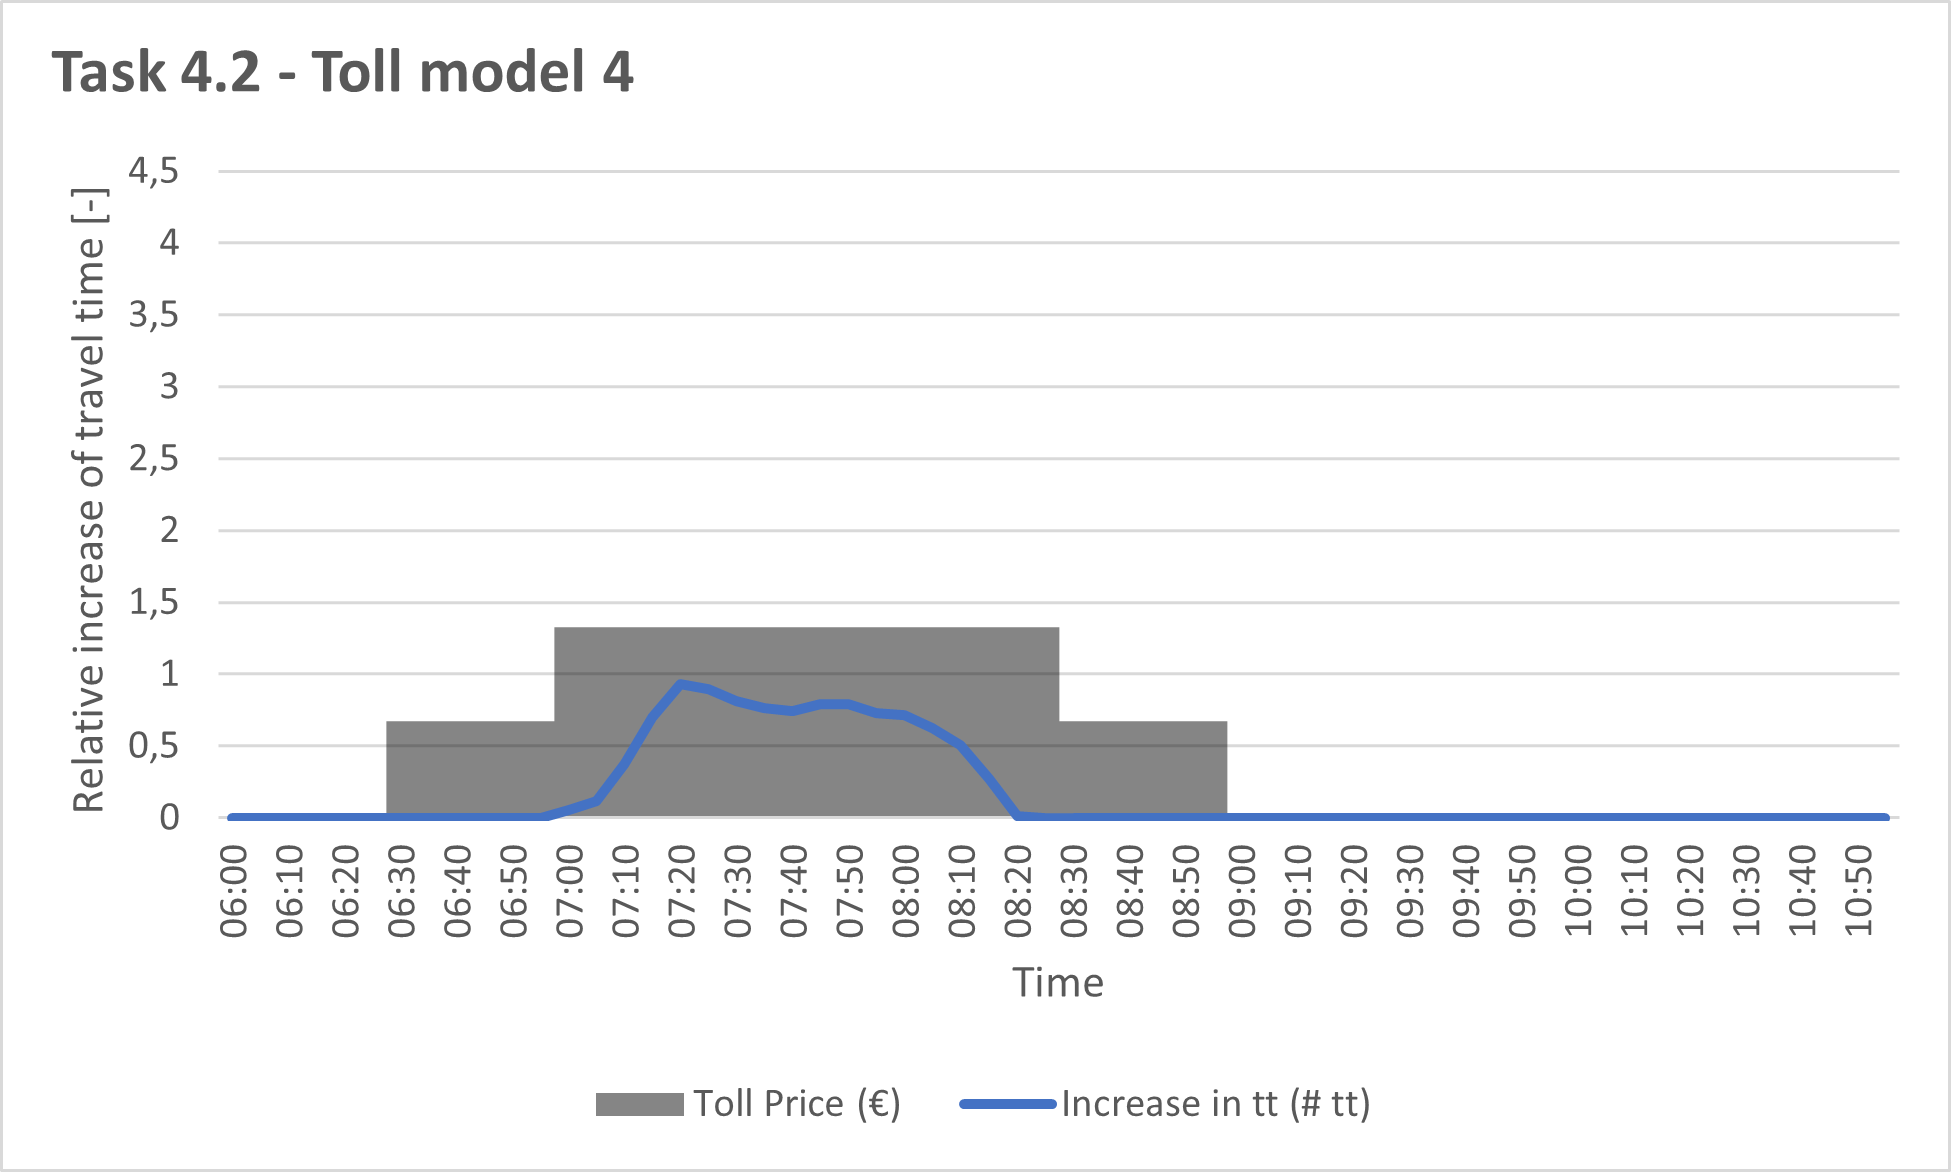
\includegraphics[width=1\textwidth]{Images/Step4/Task4.2_Toll_model_4.png}
    \caption{Relative increase of travel time with toll model 4 function of the time}
    \label{fig:Relative increase of travel time with toll model 4 function of the time}
\end{figure}
\end{minipage}
\begin{minipage}[c]{0.5\textwidth}
\begin{figure}[H]
    \centering
    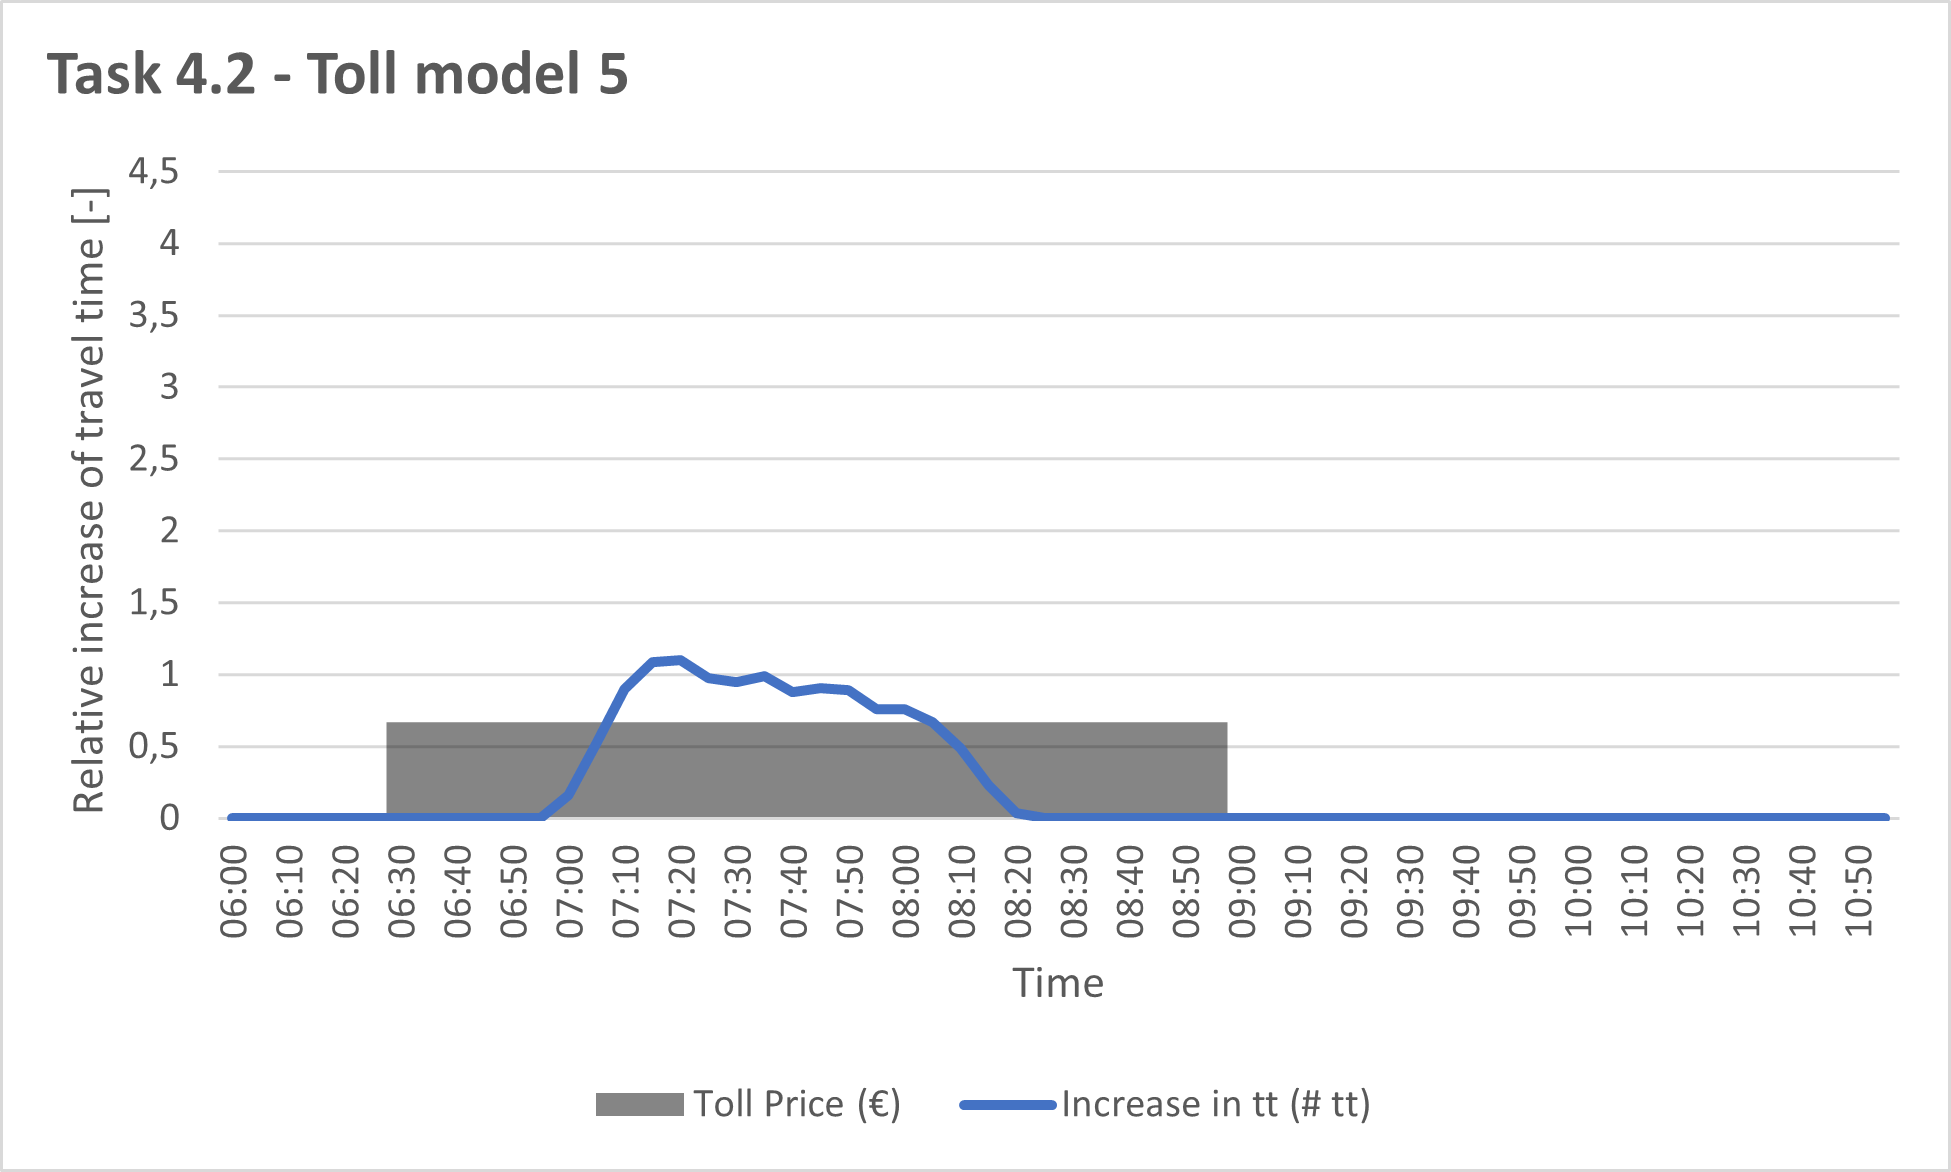
\includegraphics[width=1\textwidth]{Images/Step4/Task4.2_Toll_model_5.png}
    \caption{Relative increase of travel time with toll model 5 function of the time}
    \label{fig:Relative increase of travel time with toll model 5 function of the time}
\end{figure}
\end{minipage}
\newline

Every model is better than the model without a cordon toll or the one with a constant coll in terms of congestion.\\

However, the second model is not that good at reducing congestion compared to the other pricing model. Indeed, we notice a peak in travel time just after the end of the highest fare. We can therefore conclude that this strategy is not the most optimal one.\\

All other models divide or smooth the peak congestion into at least two smaller peaks and reduce the increase in travel time relative to the non-toll version by a factor of two, and even by a factor of three for the last three models.\\

Model 3 has the greatest impact on the level of congestion. Indeed, we see that the travel time is lower than in the other models. A small peak of congestion occurs at 06:20 am and the congestion stabilizes at a lower level until 08:15 am.\\

By removing one or two toll levels, the level at which congestion stabilizes increases. However, this has little impact on the maximum peak.\\

We can therefore deduce that the most interesting strategy of those proposed here is strategy 3. This seems perfectly logical to us.\\

Indeed, as we have seen in the course, the first best pricing is a pricing system that allows us to smooth out the peak hours. To do this, the toll price varies according to the level of congestion in order to adapt to the current situation. The ideal form of pricing would therefore be a curve similar to that of congestion. By increasing the number of tiers in our pricing diagram, we could get closer to the ideal shape and thus optimize the level of congestion.\\

However, such a toll would imply a constantly varying price (since it is indeed a continuous function). It would then be necessary to have infinitely small time intervals. This is not really feasible, since it is necessary for the user to know what price he will have to pay when he goes to the city at a certain time. A constantly changing fare is not at all realistic. So we need to find a balance between a model that is fine enough to best fit the congestion curve and a model that is simple enough to be readable and understood by users. A three-tiered pricing scheme like the one proposed here seems to us to be a good compromise.\\

It should be noted that the trial congestion charge to be implemented in the city of Geneva is also a cordon charge, and that it also has differentiated pricing according to the time of day. It is expected to apply a higher rate during peak hours and a lower rate during off-peak hours. Our model is close to this, so it is relatively realistic.\\

For the rest of this work, we will keep this third model. We will now analyze its impact on the network and compare its effects with the situation without road pricing (Task 2) and with the situation with constant pricing (Task 4.1).\\

\begin{minipage}[c]{0.5\textwidth}
\begin{figure}[H]
    \centering
    \includegraphics[width=1\textwidth]{Images/Step4/results_on_network_task4.2_700am.png}
    \caption{Entry flows in the network at 7:00 am with toll model 3 (Task 4.2)}
    \label{fig:Entry flows in the network at 7:00 am with toll model 3 (Task 4.2)}
\end{figure}
\end{minipage}
\begin{minipage}[c]{0.5\textwidth}
\begin{figure}[H]
    \centering
    \includegraphics[width=1\textwidth]{Images/Step4/results_on_network_task4.2_710am.png}
    \caption{Entry flows in the network at 7:10 am with toll model 3 (Task 4.2)}
    \label{fig:Entry flows in the network at 7:10 am with toll model 3 (Task 4.2)}
\end{figure}
\end{minipage}
\begin{minipage}[c]{0.5\textwidth}
\begin{figure}[H]
    \centering
    \includegraphics[width=1\textwidth]{Images/Step4/results_on_network_task4.2_720am.png}
    \caption{Entry flows in the network at 7:20 am with toll model 3 (Task 4.2)}
    \label{fig:Entry flows in the network at 7:20 am with toll model 3 (Task 4.2)}
\end{figure}
\end{minipage}
\begin{minipage}[c]{0.5\textwidth}
\begin{figure}[H]
    \centering
    \includegraphics[width=1\textwidth]{Images/Step4/results_on_network_task4.2_730am.png}
    \caption{Entry flows in the network at 7:30 am with toll model 3 (Task 4.2)}
    \label{fig:Entry flows in the network at 7:30 am with toll model 3 (Task 4.2)}
\end{figure}
\end{minipage}
\begin{minipage}[c]{0.5\textwidth}
\begin{figure}[H]
    \centering
    \includegraphics[width=1\textwidth]{Images/Step4/results_on_network_task4.2_740am.png}
    \caption{Entry flows in the network at 7:40 am with toll model 3 (Task 4.2)}
    \label{fig:Entry flows in the network at 7:40 am with toll model 3 (Task 4.2)}
\end{figure}
\end{minipage}
\begin{minipage}[c]{0.5\textwidth}
\begin{figure}[H]
    \centering
    \includegraphics[width=1\textwidth]{Images/Step4/results_on_network_task4.2_750am.png}
    \caption{Entry flows in the network at 7:50 am with toll model 3 (Task 4.2)}
    \label{fig:Entry flows in the network at 7:50 am with toll model 3 (Task 4.2)}
\end{figure}
\end{minipage}
\begin{minipage}[c]{0.5\textwidth}
\begin{figure}[H]
    \centering
    \includegraphics[width=1\textwidth]{Images/Step4/results_on_network_task4.2_800am.png}
    \caption{Entry flows in the network at 8:00 am with toll model 3 (Task 4.2)}
    \label{fig:Entry flows in the network at 8:00 am with toll model 3 (Task 4.2)}
\end{figure}
\end{minipage}
\begin{minipage}[c]{0.5\textwidth}
\begin{figure}[H]
    \centering
    \includegraphics[width=1\textwidth]{Images/Step4/results_on_network_task4.2_810am.png}
    \caption{Entry flows in the network at 8:10 am with toll model 3 (Task 4.2)}
    \label{fig:Entry flows in the network at 8:10 am with toll model 3 (Task 4.2)}
\end{figure}
\end{minipage}
\newline

We notice three things that are very different from the previous two situations.\\

The first (and most obvious) is that the level of congestion is much lower than before. If we analyze the situation in detail, we do notice flows converging towards the centre of the network between 7:00 am and 7:20 am, but at a much lower intensity than before. Moreover, there is no effect of strong accumulation of flows as there was with the strategy of Task 4.1. The rest of the network is similar to what was observed before.\\

Thus, although there is still a period during which the flows are a bit higher, the congestion is greatly reduced compared to previous situations.\\

The second element we can bring is that there does not seem to be a phenomenon of massive entry of vehicles at a certain time as in Task 4.1. This shows that this strategy is relevant and allows to have a real effect on congestion reduction and not only on shifting the number of passengers.\\

The third comment we can make is related to the temporal dispersion of congestion. We notice that the period during which congestion occurs is similar in the three situations. This shows that this strategy reduces the peaks but does not spread the trips over the morning.\\

This strategy is therefore favourable for reducing congestion on the network during peak hours and for limiting the number of drivers.\\


\subsubsection{Effect of the toll on congestion, customer surplus and number of public transport users}

In this section, we will compare the effects of the road pricing policy model 3 with the situation without any toll and with the toll suggested in task 4.1.\\

Again, we bring the graphs concerning congestion, consumer surplus and public transport ridership as well as travel time, speed and ratios.\\

However, this time we will show the differences between these different indicators on the last day of simulation between the analyzed method and the situation of Task 2 (where no tolls were implemented). Thus, for the no-toll strategy, the difference is zero each time. This representation allows us to better distinguish the advantages and disadvantages of each method.\\

\begin{minipage}[c]{0.5\textwidth}
\begin{figure}[H]
    \centering
    \includegraphics[width=1\textwidth]{Images/Step4/Congestion.png}
    \caption{Congestion difference with the model without any policy (Task 2)}
    \label{fig:Congestion difference with the model without any policy (Task 2)}
\end{figure}
\end{minipage}
\begin{minipage}[c]{0.5\textwidth}
\begin{figure}[H]
    \centering
    \includegraphics[width=1\textwidth]{Images/Step4/Surplus.png}
    \caption{Consumer surplus difference with the model without any policy (Task 2)}
    \label{fig:Consumer surplus difference with the model without any policy (Task 2)}
\end{figure}
\end{minipage}
\begin{minipage}[c]{0.5\textwidth}
\begin{figure}[H]
    \centering
    \includegraphics[width=1\textwidth]{Images/Step4/TravelTime.png}
    \caption{Travel time difference with the model without any policy (Task 2)}
    \label{fig:Travel time difference with the model without any policy (Task 2)}
\end{figure}
\end{minipage}
\begin{minipage}[c]{0.5\textwidth}
\begin{figure}[H]
    \centering
    \includegraphics[width=1\textwidth]{Images/Step4/Speed.png}
    \caption{Speed difference with the model without any policy (Task 2)}
    \label{fig:Speed difference with the model without any policy (Task 2)}
\end{figure}
\end{minipage}
\begin{minipage}[c]{0.5\textwidth}
\begin{figure}[H]
    \centering
    \includegraphics[width=1\textwidth]{Images/Step4/Ratios.png}
    \caption{Ratios differences with the model without any policy (Task 2)}
    \label{fig:Ratios differences with the model without any policy (Task 2)}
\end{figure}
\end{minipage}
\begin{minipage}[c]{0.5\textwidth}
\begin{figure}[H]
    \centering
    \includegraphics[width=1\textwidth]{Images/Step4/Travelers.png}
    \caption{Number of travellers by category differences with the model without any policy (Task 2)}
    \label{fig:Number of travelers by category differences with the model without any policy (Task 2)}
\end{figure}
\end{minipage}
\\
\newline
The introduction of the Model 3 pricing policy has a positive impact on almost all the indicators compiled above compared to the situation without the road pricing policy.\\

In total, 9\% of the initial congestion is avoided whereas, with the strategy proposed in Task 4.1, there was a 5\% increase in congestion. However, as in Task 4.1, the consumer surplus is worse with a toll. This was also the case with the strategy analyzed earlier at the beginning of Task 4. This can be explained by the fact that individually and in the short run, the addition of a toll represents an additional cost to the population compared to the previously stabilized situation. Thus, whatever pricing strategy is put in place, the situation will always be worse than in the base case. Note, however, that the consumer surplus is higher with strategy 3 (-0.068 €) than with the base strategy (-0.224 €).\\

Because there is a decrease in congestion with model 3, there is a higher speed (+2.8 (km/h)) and, consequently, a travel time gain (-1.1 (min)). The evolution is the opposite of the previous model.\\

Concerning the ratios, we note a decrease in early arrivals (-2.5 (\%)), an increase in on-time arrivals (+2.3 (\%)) and a very small increase in late arrivals (+0.18 (\%)). Thus, we see that this strategy is highly desirable because, in addition to decreasing congestion in the network during peak hours, it also decreases the number of arrivals that are off schedule. This is because of the dispersion of travellers, which decreases congestion and thus travellers can leave at a time more consistent with their arrival time.\\

In Figure \ref{fig:Number of travelers by category differences with the model without any policy (Task 2)}, we can see that few travellers switch from car to public transport. This indicates that travellers prefer to shift their departure time rather than change modes. There was a greater modal shift with Task 4.1 pricing because the measure was much blunter.\\

As we saw in the Task 4.1 section, the situation with this toll proposal is worse than the initial situation in all statistics. This indicates that the introduction of a road pricing policy must be well thought out and prepared, as it can lead to a worse situation.

The statistics in Task 4.1 show that the situation with this toll proposal is worse than the initial situation in all statistics. This indicates that the introduction of a road pricing policy has to be well thought out and prepared because it can lead to a worse situation.\\


We also tried an extreme case with a constant toll of 10 €. The congestion is actually reduced but the consumer surplus become unbearable, so this policy is not enforceable in reality.
\begin{minipage}[c]{0.5\textwidth}
\begin{figure}[H]
    \centering
    \includegraphics[width=1\textwidth]{Images/Step4/Task4.2_Toll_model_6.png}
    \caption{Relative increase of travel time with toll model 6 function of the time}
    \label{fig:Relative increase of travel time with toll model 6 function of the time}
\end{figure}
\end{minipage}
\begin{minipage}[c]{0.5\textwidth}
\begin{figure}[H]
    \centering
    \includegraphics[width=1\textwidth]{Images/Step4/Surplus7.png}
    \caption{Consumer surplus differences with the model without any policy (Task 2)}
    \label{fig:Consumer surplus differences with the model without any policy (Task 2) model 6}
\end{figure}
\end{minipage}



\section{Conclusion}

The goal of this lab was to get used to a specific dynamic traffic simulator, METROPOLIS. By familiarizing with the characteristic of the program and how it works. We used a circular city network with four rings.\\

During the first task, we were able to understand and interpret the outputs of a simple simulation in task 2. By this simulation, congestion occurred during the peak hours, i.e. between 6:45 am and 8:30 am, particularly in the city centre.\\

Then, by adding a second type of traveller, we described the impact of the input parameters on the simulation in task 3. By adding a so-called "Low-Income Traveler", the level of congestion decreased slightly and benefits all the network users. However, in reality, this rises socio-economic interrogation about the inequality of access to the network between populations with differentiated incomes. This is beyond the scope of this lab but has to be kept in mind.\\

Eventually, we tried several road pricing policies and characterize their effect on the network and the outputs of the simulation. Generally speaking, introducing road pricing policies reduces the level of congestion, which is beneficial to the whole network. But on the other hand, the consumer surplus is downgraded by every toll model. Indeed, this introduction results in and increase in the cost for the travellers, that are at least in short term not and in that simulation not compensated by the reduction of congestion and travel time. But this doesn't mean that introduction of road pricing policy is always harmful. This simulation only focuses on the transportation cost and values of time. But the reduction of congestion and road pricing policies can have a lot of indirect benefits, from the improvement of public health to a call to action to use more sustainable modes of transportation. \\

Using a simulation program is important to understand fully the impact of policies and socio-economic characteristics on transportation networks and guide the decision-making process.

\end{document}
